\documentclass[twoside,11pt,openright]{report}

\usepackage[latin1]{inputenc}
\usepackage[english]{babel}
\usepackage{a4}
\usepackage{latexsym}
\usepackage{amssymb}
\usepackage{amsmath}
\usepackage{mathtools}
\usepackage{epsfig}
\usepackage[T1]{fontenc}
\usepackage{lmodern}
\usepackage{color}
\usepackage{datetime}
\usepackage{epstopdf}
\usepackage{textcomp}

% This font looks so good.
\usepackage[sc]{mathpazo}

% Typesetting pseudo-code
\usepackage{algorithm}
\usepackage{algorithmic}
\usepackage{multirow}

% Inline list
\usepackage[inline]{enumitem}
\newlist{inlinelist}{enumerate*}{1}
\setlist[inlinelist]{label=(\roman*)}

% tikz
\usepackage{tikz}
% git graph
\newcommand\commit[3]{\node[commit] (#1) {}; \node[clabel] at (#1) {\texttt{#1}: (\textit{#2}) #3};}
\newcommand\ghost[1]{\coordinate (#1);}
\newcommand\connect[2]{\path (#1) to[out=90,in=-90] (#2);}

% Code comments like [CLRS]
\renewcommand{\algorithmiccomment}[1]{\makebox[5cm][l]{$\triangleright$ \textit{#1}}}
\usepackage{framed,graphicx,xcolor}
\usepackage[space]{grffile}
\usepackage[font={small,it}]{caption}
\usepackage{listings}
\usepackage{units}

% theorems
\newtheorem{theorem}{Theorem}
\newtheorem{definition}{Definition}
\newtheorem{lemma}{Lemma}

% Relative references
\usepackage{varioref}

\usepackage[hidelinks]{hyperref}
\usepackage{url}

% Set fonts for section
\usepackage{titlesec}
\titleformat*{\section}{\LARGE\bfseries}
\titleformat*{\subsection}{\large\bfseries}

\bibliographystyle{alpha}

\renewcommand*\ttdefault{txtt}

\newcommand{\todo}[1]{{\color[rgb]{.5,0,0}\textbf{$\blacktriangleright$#1$\blacktriangleleft$}}}

% \newcites{A,B}{Primary Bibliography,Secondary Bibliography}

% see http://imf.au.dk/system/latex/bog/

\begin{document}

\pagestyle{empty} 
\pagenumbering{roman} 
\vspace*{\fill}\noindent{\rule{\linewidth}{1mm}\\[4ex]
{\Huge\sf Three-sided Range Reporting}\\[2ex]
{\huge\sf Peter Gabrielsen, 20114179}\\[2ex]
{\huge\sf Christoffer Holb\ae k Hansen, 20114637}\\[2ex]
\noindent\rule{\linewidth}{1mm}\\[4ex]
\noindent{\Large\sf Master's Thesis, Computer Science\\[1ex] 
\monthname\ \the\year  \\[1ex] Project Advisor: Kasper Green Larsen
\\[1ex] Formal Advisor: Gerth St\o lting Brodal\\[15ex]}\\[\fill]}

\epsfig{file=logo.eps}\clearpage

%%%%%%%%%%%%%%%%%%%%%%%%%%%%%%%%%%%%%%%%%%%%%%%%%%%%%%%%%%%%%%%%%%%%%%%

\pagestyle{plain}
\chapter*{Abstract}
\addcontentsline{toc}{chapter}{Abstract}

\todo{in English\dots}

\chapter*{Resum\'e}
\addcontentsline{toc}{chapter}{Resum\'e}

\todo{in Danish\dots}

\chapter*{Acknowledgements}
\addcontentsline{toc}{chapter}{Acknowledgements}

\todo{\dots}

\vspace{2ex}
\begin{flushright}
  \emph{Peter Gabrielsen and Christoffer Holb\ae k Hansen}\\
  \emph{Aarhus, \today.}
\end{flushright}

\tableofcontents

\chapter*{Preface}
\label{chp:preface}
\addcontentsline{toc}{chapter}{Preface}
\todo{mention star wars and scaring the crap out of C}

\todo{Getting hot in here}

\todo{number of lines of code}
\begin{figure}
\centering
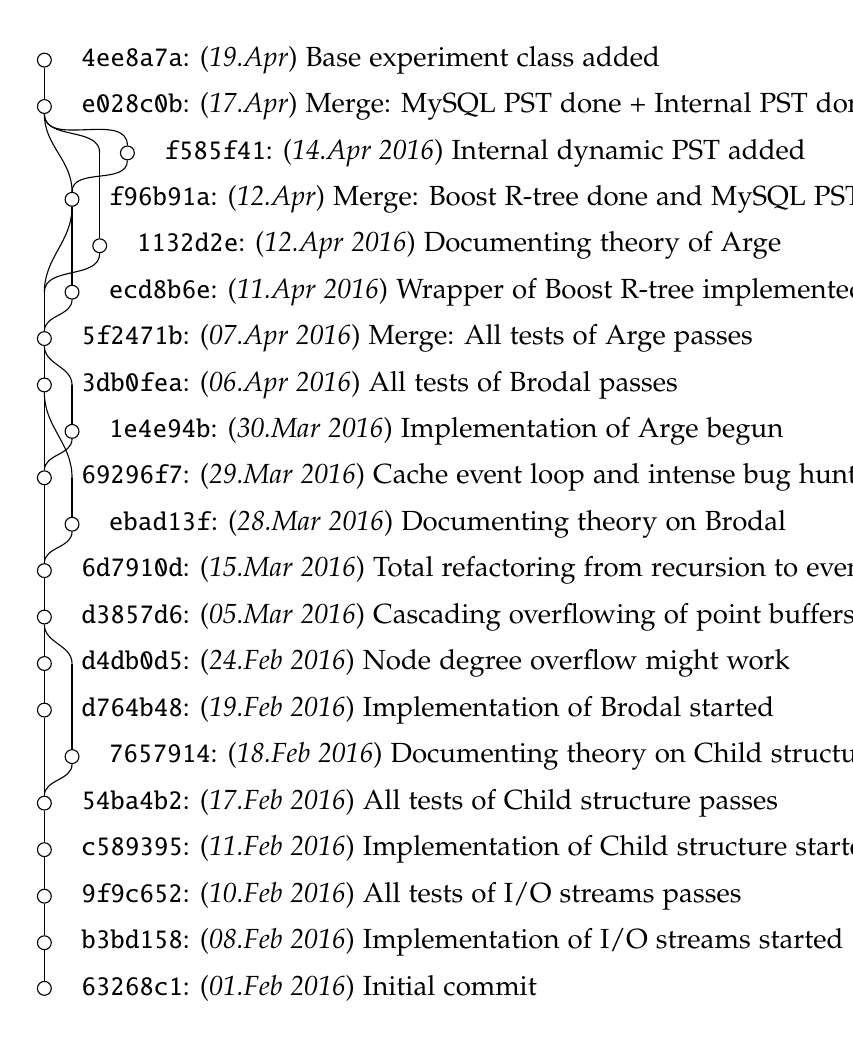
\begin{tikzpicture}
\tikzstyle{commit}=[draw,circle,fill=white,inner sep=0pt,minimum size=5pt]
\tikzstyle{clabel}=[right,outer sep=1em]
\tikzstyle{every path}=[draw]
\matrix [column sep={1em,between origins},row sep=\lineskip]
{
\commit{4ee8a7a}{19.Apr}{Base experiment class added} & \\
\commit{e028c0b}{17.Apr}{Merge: MySQL PST done + Internal PST done} & \\
& & \ghost{branch6} & \commit{f585f41}{14.Apr 2016}{Internal dynamic PST added} \\
& \commit{f96b91a}{12.Apr}{Merge: Boost R-tree done and MySQL PST started} & & \\
& \ghost{branch5} & \commit{1132d2e}{12.Apr 2016}{Documenting theory of Arge} \\
\ghost{branch4} & \commit{ecd8b6e}{11.Apr 2016}{Wrapper of Boost R-tree implemented} \\
\commit{5f2471b}{07.Apr 2016}{Merge: All tests of Arge passes} & \\
\commit{3db0fea}{06.Apr 2016}{All tests of Brodal passes} & \ghost{branch3} \\
& \commit{1e4e94b}{30.Mar 2016}{Implementation of Arge begun} \\
\commit{69296f7}{29.Mar 2016}{Cache event loop and intense bug hunting} & \ghost{branch2} \\
& \commit{ebad13f}{28.Mar 2016}{Documenting theory on Brodal} \\
\commit{6d7910d}{15.Mar 2016}{Total refactoring from recursion to event loop} & \\
\commit{d3857d6}{05.Mar 2016}{Cascading overflowing of point buffers} & \\
\commit{d4db0d5}{24.Feb 2016}{Node degree overflow might work} & \ghost{branch1}\\
\commit{d764b48}{19.Feb 2016}{Implementation of Brodal started} & \\
& \commit{7657914}{18.Feb 2016}{Documenting theory on Child structure} \\
\commit{54ba4b2}{17.Feb 2016}{All tests of Child structure passes} & \\
\commit{c589395}{11.Feb 2016}{Implementation of Child structure started} & \\
\commit{9f9c652}{10.Feb 2016}{All tests of I/O streams passes} & \\
\commit{b3bd158}{08.Feb 2016}{Implementation of I/O streams started} & \\
\commit{63268c1}{01.Feb 2016}{Initial commit}& \\
};
\connect{63268c1}{b3bd158};
\connect{b3bd158}{9f9c652};
\connect{9f9c652}{c589395};
\connect{c589395}{54ba4b2};
\connect{54ba4b2}{d764b48};
\connect{54ba4b2}{7657914};
\connect{7657914}{branch1};
\connect{branch1}{d3857d6};
\connect{d764b48}{d4db0d5};
\connect{d4db0d5}{d3857d6};
\connect{d3857d6}{6d7910d};
\connect{6d7910d}{ebad13f};
\connect{6d7910d}{69296f7};
\connect{ebad13f}{branch2};
\connect{branch2}{3db0fea};
\connect{69296f7}{1e4e94b};
\connect{1e4e94b}{branch3};
\connect{branch3}{5f2471b};
\connect{3db0fea}{5f2471b};
\connect{69296f7}{3db0fea};
\connect{5f2471b}{ecd8b6e};
\connect{5f2471b}{branch4};
\connect{branch4}{f96b91a};
\connect{branch4}{1132d2e};
\connect{f96b91a}{f585f41};
\connect{ecd8b6e}{branch5};
\connect{branch5}{f96b91a};
\connect{f96b91a}{e028c0b};
\connect{f585f41}{e028c0b};
\connect{1132d2e}{branch6};
\connect{branch6}{e028c0b};
\connect{e028c0b}{4ee8a7a};
\end{tikzpicture}
\caption{Excerpt of git history for the entire project}
\end{figure}

\pagenumbering{arabic}
\setcounter{secnumdepth}{2}

\chapter{Introduction}
\label{chp:introduction}
% words: big data, banking, data larger than memory, database community, slow disks, disparity between growth of CPU speeds and transfer speeds between internal and external memory (widening gap)
% fault tolerance and consistency are more challenging to handle in-memory (In-Memory Big Data Management and Processing: A survey)
% storage prices
% The I/O bottleneck
% Disk were faster than CPU in 60
% http://read.cs.ucla.edu/111/2006fall/notes/lec15#incommensurate-scaling

In the early days of electronic computers disks were faster than processors. Since then processor technology has advanced at an incredible rate achieving annual speedups of 40 to 60 percent~\cite{ruemmler_wilkes_1994}. Although this is also true for disk capacity an entirely different story can be told for the speedup of disk performance. The disparity between processor, internal memory, and external memory speeds have grown larger for each year and the gap is widening as seen in figure~\ref{fig:cpu_vs_disk}. A back on the envelope analysis shows that a job that was 5 \% disk bound in 1999 is more than 70 \% disk bound on an average CPU in 2014. This disparity presents serious problems when designing algorithms on large data sets, and with more and more applications of Big Data in social media, banking, etc., these problems become increasingly relevant.

\begin{figure}[h]
	\centering
		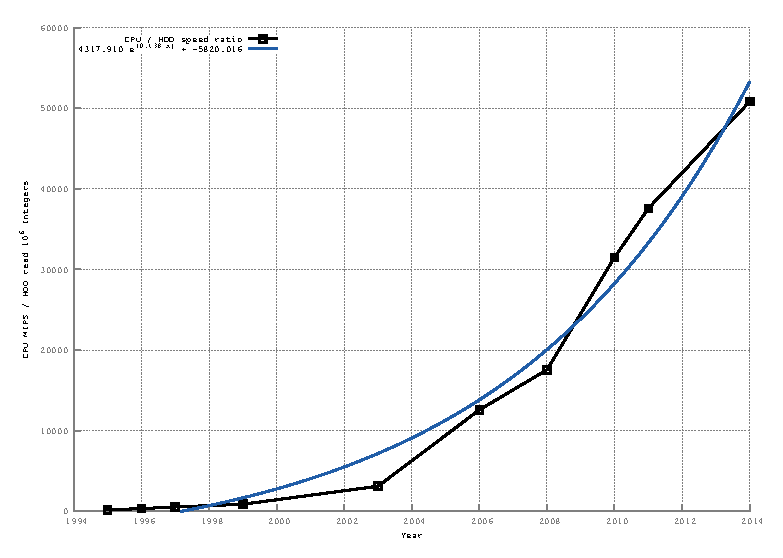
\includegraphics[width=\textwidth]{../plots/scaling_discrepancy_hdd_cpu/scaling_discrepancy_hdd_cpu}
	\caption{Growth of CPU and HD speed ratio over time.}
	\tiny{Data found at~\protect\url{https://en.wikipedia.org/wiki/Instructions_per_second}}
	\label{fig:cpu_vs_disk}
\end{figure}

While the database community has always been involved in the development of practically efficient external memory data structures, most algorithms research has focused on worst-case efficient internal memory data structures. With the advent of Big Data and problems concerning large data sets the algorithms community has been increasingly involved in developing worst-case efficient external memory data structures for solving these problems~\cite{ionote}.

%TODO reformulate.
To some large internet companies, disk-based systems presents too large of an obstacle, and in an attempt to close the gap they have moved towards developing internal memory big data processing algorithms. This move has been enabled by growing main memory capacities but it comes with the price of issues such as fault-tolerance and consistency which are inherently more challenging to handle in volatile memory~\cite{Zhang2015}.

Another price of this move to internal memory is the actual cost of running server farms and the cost of internal memory compared to external memory. The extra costs and increased complexity suggests that external memory data structures have some well defined advantages.

An integral problem of computational geometry is that of range searching. The problem arises in many different applications with huge data sets such as geographic information systems, spatial databases, and computer graphics. The problem can be formally described as follows. Let $\mathcal{S}$ be a set of $N$ points in $\mathbb{R}^d$, and let $\mathcal{R}$ be a family of subsets of $\mathbb{R}^d$. Our objective is to preprocess $\mathcal{S}$ such that for a query range $r \in \mathcal{R}$, the points in $\mathcal{S} \cap r$ can be reported or counted efficiently~\cite{Agarwal99geometricrange}. The ranges can be anything from rectangles and halfspaces to balls.

In this thesis we consider the problem of maintaining a dynamic set, $\mathcal{S}$, of $N$ points in $\mathbb{R}^2$ in external memory. The set of points can be updated by insertion and deletion. The set will be processed such that we are able to report three-sided range queries, i.e. given a range of the type $[x_1,x_2] \times [y,\infty]$, we report points in $\mathcal{S} \cap [x_1,x_2] \times [y,\infty]$.

\begin{figure}[h]
	\centering
	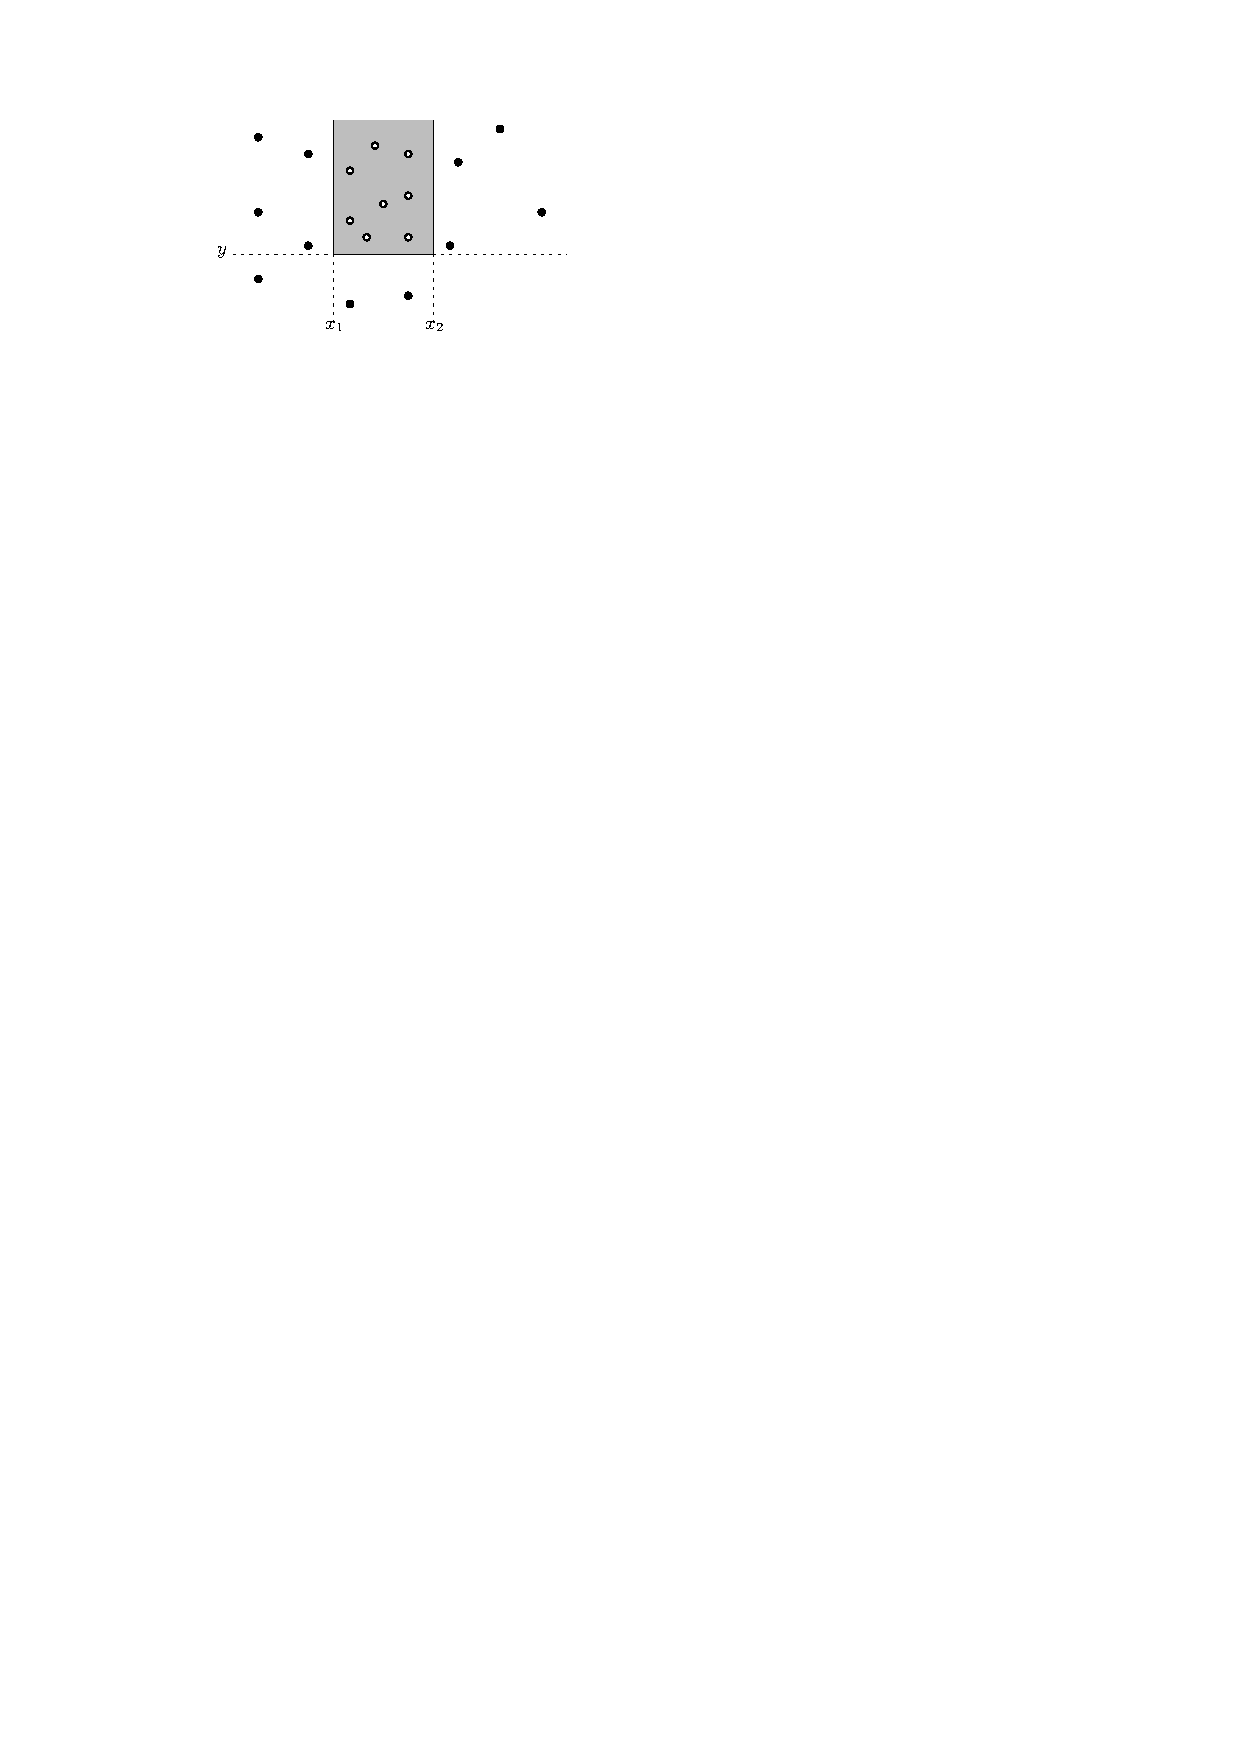
\includegraphics[scale=1]{../figures/three-sided-query}
	\caption{A query of the form $[x_1,x_2] \times [y,\infty]$, reporting all points in the grey area.}
	\label{fig:three-sided-query}
\end{figure}
 
The thesis will present several solutions to this problem, implement, and experimentally compare solutions.

Some of the solutions will not be optimized for usage in external memory and they must pay a hefty price for accessing data not readily available in main memory. This thesis will show the power of the I/O efficient data structures for large data sets and demonstrate what happens when internal memory data structure have to work overtime along with the virtual memory system.

The different solutions will be analyzed in the I/O model which encapsulates performance as number of disk accesses as opposed to RAM accesses. Further details on the I/O model is described in Chapter~\ref{chp:iomodel}.

\section{Outline of thesis}
This thesis is structured as follows:

In Chapter~\ref{chp:iomodel} we investigate a model that encapsulates performance of the I/O bottleneck.

In Chapter~\ref{chp:prelims} we give a preliminary overview of some of the techniques used in developing external memory efficient data structures.

Much work has been done on the three sided range queries and more general range queries. Some of the main ideas leading up to the main focus of this thesis is presented in Chapter~\ref{chp:related_work}.

Chapter~\ref{chp:internal_pst} gives a detailed description and analysis of the priority search tree for internal memory by McCreight~\cite{DBLP:journals/siamcomp/McCreight85}.

The main focus of this thesis, the external memory buffered priority search tree of Brodal~\cite{DBLP:journals/corr/Brodal15} is presented in Chapter~\ref{chp:epst}.

\todo{add more sections!}

\chapter{Model of computation}
\label{chp:iomodel}
We will argue the results of this thesis in terms of the external memory model of Aggarwal and Vitter~\cite{Aggarwal:1988/ICS/48529.48535}.
The external memory model (or I/O model) measures the efficiency of an algorithm by counting the total number of reads and writes performed. In detail the model consists of two levels of memory; a bounded internal memory of size $M$ and an unbounded external memory. For a total of $N$ records we define an \textit{I/O} operation to the process of transferring $B$ consecutive records between the two levels of memory as depicted in figure~\ref{fig:io_model}. We restrict all computations on records to be done in internal memory. Throughout the thesis we will let $K$ denote the total number of records in the output.

\begin{figure}[h]
	\centering
	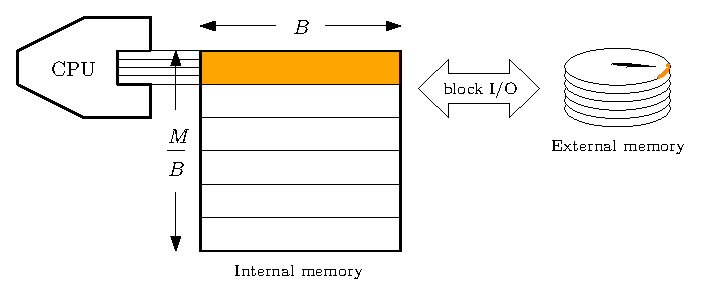
\includegraphics[width=1\textwidth]{../figures/block_io}
	\caption{The I/O Model. Only reads/writes between internal and external memory are charged.}
	\label{fig:io_model}
\end{figure}

The fundamental bounds in the external memory model is that scanning can be done in $\mathcal{O}(\text{Scan}) = \mathcal{O}(\nicefrac{N}{B})$, sorting in $\mathcal{O}(\text{Sort}) = \mathcal{O}(\nicefrac{N}{B} \log_{\nicefrac{M}{B}}\nicefrac{N}{B})$ and searching in $\mathcal{O}(\log_B N)$. We denote $\mathcal{O}(\nicefrac{N}{B})$ as being linear in terms of I/Os. Note that the $B$ factor is very important as $\nicefrac{N}{B} < \mathcal{O}(\nicefrac{N}{B} \log_{\nicefrac{M}{B}}\nicefrac{N}{B}) \ll N$.

For convenience we will assume $M > B^2$. This assumption is known as the \textit{tall-cache assumption} in the cache-oblivious model and basically states that the number of blocks \nicefrac{M}{B} is larger than the size of each block $B$~\cite{Prokop99cache-obliviousalgorithms}.

\chapter{Preliminaries}
\label{chp:prelims}
This section aims to give an overview of some of the techniques used throughout this thesis. Some of the techniques are very rudimental and may be skipped or revisited when encountered in later sections.

\section{Amortization}
Amortization is an important algorithmic tool to argue about average performance of an operation in the worst case.
In an amortized analysis, we average the time of a sequence of data structure operations. We can then show that, even though a single operation in the sequence is expensive, the average cost of an operation is small~\cite[p.~451-452]{clrs}.

The term was coined by Tarjan~\cite{Tarjan85} and describes two views of amortization. The first view is the banker's view where we assume that a computer is running on coins. We can insert a coin and the computer will run for fixed constant amount of time. An operation will pay a certain amounts of coins and the goal of the analysis is then to show that all operations can be performed with the amount paid. We assume that we start without any coins, we are allowed to borrow coins, and coins can be carried over to later operations. Paying coins amounts to averaging forward over time and borrowing is the opposite.

Another view of amortization is that of the physicist. Instead of representing prepaid work as coins the physicist represent work as potential energy which can be released later to pay for future operations.

If we perform $n$ operations, we will start with an initial data structure $D_0$. For each of the operations we let $c_i$ be the cost of operation $i$ and $D_i$ be the data structure that results from that operation on the previous data structure. We define a potential function $\Phi$ to map a data structure $D_i$ to a real number $\Phi(D_i)$. The cost of the $i$th operation becomes
$$\hat{c}_i = c_i + \Phi(D_i) - \Phi(D_{i-1})$$
The total amortized cost becomes
\begin{align*}
\sum_{i=1}^n \hat{c}_i &= \sum_{i=1}^n c_i + \Phi(D_i) - \Phi(D_{i-1}) \\
&= \sum_{i=1}^n c_i + \Phi(D_n) - \Phi(D_{0})
\end{align*}

If we can show that $\Phi(D_i) \geq \Phi(D_0)$ for all $i$ then we know that we always are able to build up enough potential in advance.

\section{Global rebuilding}
\label{sec:prelim_global_rebuilding}
The term \textit{global rebuilding} refers to the standard technique of making a (typically small) static data structure dynamic. We simply store all updates in a \textit{update block} and once a certain threshold has been collected we rebuild the data structure~\cite{ionote}. For data structures that does not allow the space for deleted records to be reoccupied we \textit{mark} (or \textit{weak delete}) the elements. Whenever $\alpha N$ elements have been marked, for some constant $\alpha > 0$, the entire data structure is rebuilt from scratch with only the non-marked elements. The cost of rebuilding is at most a constant factor higher than the cost of inserting $\alpha N$ elements and so the amortized cost of global rebuilding can be charged to the insertions of the deleted elements~\cite{Meyer:2003/AMH/1744652}.

\section{Filtering}
\label{sec:filtering}
The technique of \textit{filtering} is used on retrieval problems where we query a certain data structure for a subset of data points. The technique is based on the fact that the complexity of the \textit{search} and the \textit{report} parts of the algorithm should be made dependent upon each other such that we charge part of the query cost to output. In order to make filtering search feasible, it is crucial that the problems specifically require the exhaustive enumeration of the objects satisfying the query.

\section{Bootstrapping}
It is often possible to develop dynamic external memory data structures by "externalizing" the equivalent internal memory data structure. In the case of trees this typically involves increasing the fanout from binary to multiway. This, however, results in problems when searching and reporting items from the tree, e.g. it might be the case that each subtree of a node only contributes one item to the query answer each costing one I/O.

This problem can sometimes be solved by augmenting the data structure with several filtering substructures, i.e. smaller versions of the same problem. This approach was first described by Arge and Vitter~\cite{arge_vitter_2003} in a paper giving an optimal solution to diagonal corner two-sided 2D queries. Each of the substructures typically holds $\mathcal{O}(B^2)$ elements, and answers queries in $\log_B B^2 + \nicefrac{K}{B}$, where $K$ is the size of the output. It can even be a static structure if it can be constructed in $\mathcal{O}(B)$ I/O's, since $B$ updates can be stored in a separate buffer and applied using a global rebuild in amortized $\mathcal{O}(1)$ I/O's per update~\cite{vitter_2008}.

\section{B-tree}
\label{sec:prelim_b_tree}
The B-tree of Bayer and McCreight~\cite{bayer_mccreight_1972} is to external memory what the balanced binary search tree is to internal memory. It supports insertions and deletions of points, and searching in $\mathcal{O}(h)$ where $h$ is the height of the tree. The height of the tree depends on the branching parameter, i.e. the maximum number of children a node can have. This parameter typically depends on the characteristics of the disk used and the problem at hand. 
This gives the following definition of a B-tree:

\begin{definition}
\label{def:btree}
$\mathcal{T}$ is a B-tree with branching parameter $b$ if
\begin{itemize}
	\item All leaves have the same depth
	\item All nodes store at most $b-1$ elements.
	\item All nodes and leaves except for the root have degree between $\frac{1}{2}b$ and $b$.
	\item The root has degree between $2$ and $b$.
	\item Elements are stored in non-decreasing order in the nodes.
	\item The keys of node $x$, $x.key_i$, separate the children's elements into ranges such that if $k_i$ is a key stored in child $c_i$ then $k_1 \leq x.key_1 \leq k_2 \leq x.key_2 \leq \cdots$
\end{itemize}
\end{definition}

\begin{figure}[h]
	\centering
	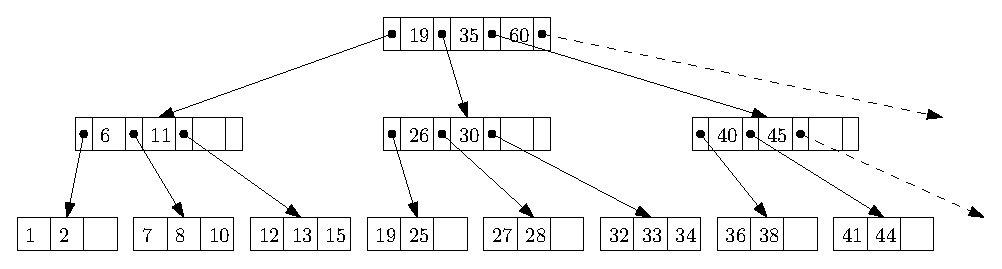
\includegraphics[width=\textwidth]{../figures/b-tree}
	\caption{A B-tree with $b = 4$}
	\label{fig:b-tree}
\end{figure}

It follows from the definition that if $b=\Theta(B)$ then a B-tree will have height $\mathcal{O}(\log_B N)$.

\textbf{Searching} in a B-tree is very much similar to searching in a binary search tree. Instead of making a binary decision at each node we instead have to make a multiway branching decision. If the element we are searching for is not contained in the current node, we find the smallest $i$ such that the key we are searching for is less than $x.key_i$. We then recursively search for the key in child $c_i$. This will in the worst case require $\mathcal{O}(\log_B N)$ I/O to search for an element residing in a leaf.

\textbf{Inserting} in a B-tree is not as simple as inserting into a binary search tree. Similarly to binary trees we search for the leaf node to insert the key, but we cannot simply create a new node for the key. Instead we insert the key into the found leaf node and if the leaf now contains too many elements we split the leaf into two leaves each containing half the elements of the original leaf. Splitting a leaf might cause its parent to have too many children which causes the parent to similarly split.
Searching for the leaf node to insert into takes $\mathcal{O}(\log_B N)$ and so does recursively splitting nodes from a leaf to root path as a split operation requires $\mathcal{O}(1)$ I/O's.

\textbf{Deleting} in a B-tree introduces an opposite to splitting, fusing. To delete a key from the tree we search the tree for the key, which now can reside in an internal node. We then delete the key from the node $x$, which might cause $x$ to have too few elements. To remedy this situation we will have to potentially fuse $x$ with a neighbouring node. If $x$ together with either its predecessor or successor contains less than $b$ elements we can fuse the two nodes. If this is not the case then we know that we are able to steal an element from a neighbouring node in order to satisfy the properties of the B-tree. As in the case of insertion, fusing nodes might recursively cause the parent to fuse with one of its neighbours.
Fusing two nodes require $\mathcal{O}(1)$ I/O's but a fuse can cascade from a leaf to root path causing $\mathcal{O}(\log_B N)$ I/O's.

A B-tree on $N$ elements are stored in $\mathcal{O}(\nicefrac{N}{B})$ blocks and can be constructed in the sorting bound.

\todo{Maaske lav nogle figurer}

\section{Buffer tree}
\label{sec:prelim_buffer_tree}
The Buffer Tree of Arge~\cite{Arge:1995:BTN:645930.672850} combines the basic B-Tree with a \textit{buffer-technique} that will be introduced shortly. The result is an external data structure supporting batched operations I/O efficiently. The ideas introduced by Arge has proven especially useful when generalizing well-known internal-memory algorithms into efficient I/O algorithms. The main idea of the buffer-technique is to introduce \textit{laziness} in the update algorithms and utilizing main memory to process a large number of updates simultaneously. For example, when inserting a point we do not search all the way down the tree to find the leaf. Instead, the point is inserted into a buffer of the root. Whenever the size of a buffer exceeds a certain threshold we push elements from the buffer one level down to buffers on the next level of the tree. This process of emptying full buffers is repeated recursively down the tree.

Formally the basic Buffer tree is defined as follows:

\begin{definition}
\label{def:buffer_tree}
A basic buffer tree $\mathcal{T}$ is
\begin{itemize}
	\item A B-tree with branching parameter $\nicefrac{M}{B}$ and leaf parameter $B$
	\item Each internal node has a buffer of size $M$
\end{itemize}
\end{definition}

\textbf{Updates} are handled handled by augmenting the element in question with information on whether we are inserting or deleting. Since an element can be represented in multiple buffers, we also augment elements with a time stamp.
Whenever we have collected $B$ elements we insert all of them into the root buffer of size $M$. Whenever the buffer overflows, i.e. have more than $M$ points, we initiate a buffer-emptying process that distributes all elements in the buffers to the children.

For an \textit{internal} node that do not have leaves as children this process is done as follows. First, we load the $M$ unsorted elements into main memory and sort them. Then we scan through the sorted list while removing matching inserts and deletes with respect to the time stamps of each element. Now we simply scan distribute the remaining elements one level down. We make sure to distribute the elements in sorted order, since this will guarantee that we leave no buffer of a child with more than $M$ unsorted elements followed by list of sorted elements. Thus, we are able to sort the resulting buffer in a linear number of I/O's.

We then recursively empty full child buffers provided the children are internal nodes that do not have leaves as children. Only when we have emptied buffers of all overflowing internal nodes which does not have leaves as children, we proceed and process the buffer-emptying process to leave nodes. The reason is that a buffer-emptying process on a leaf node may result in the need for rebalancing. By only emptying leaf nodes after all internal node buffer-emptying processes have been performed we prevent rebalancing and buffer-emptying processes from interfering with each other.

We empty all relevant leaf nodes buffers one-by-one while maintaining the \textit{leaf-emptying invariant} that all buffers of nodes on the path from root of $\mathcal{T}$ to a leaf node with full buffer are empty. Since we handle all internal nodes before emptying the leaf nodes this invariant is true when we handle the buffer-emptying of the first leaf. To empty a node $u$ with $K$ elements in the leaves, we start by sorting the buffer and remove matching inserts and deletes. Then, we merge the buffer elements with the $K$ leaves below, again removing matching inserts and deletes. The resulting set of $K'$ sorted elements now needs to replace the $K$ original leaves along with new routing elements of $u$ reflecting the changes. If we end up with a resulting set of size $K' < K$, i.e. we do not have enough elements to fill the $K$ leaves, we introduce $K-K'$ dummy elements and insert those in the remaining leaves. If we have $K' \geq K'$ we place $K$ elements in the leaves. The remaining (if any) are finally placed one-by-one and rebalance the B-tree when necessary. We can rebalance as normally using splits as depicted in figure \todo{reference to figure that should be placed in B-tree section}, since the leaf emptying invariant insures that all nodes from $u$ to the root of $\mathcal{T}$ have empty buffers.

After we have emptied all leaf-node buffers we remove the placeholder-elements one-by-one. The leaf-emptying invariant ensures that a node $v$ on the path from $u$ to the root has an empty buffer, but $v's$ siblings may not have empty buffers. Therefore we can not fuse in a normal B-tree manner. Instead, we perform a buffer-emptying process on $v's$ immediate sibling(s) before performing the actual fuse. Note that we empty the buffers of both immediate siblings of $v$ because insert rebalancing may result in one of them having the same parent as $v$. This happens if the parent of $v$ splits.

The emptying of the buffer of a sibling node $v'$ can result in buffers running full. We empty all such full non-leaf buffers before performing the actual fuse on $v$. The place-holder elements ensures we are always only in the process of handling a rebalancing caused by a single delete.

\subsection{Analysis}
Emptying an internal node buffer of size $X$ takes $\mathcal{O}(\nicefrac{X}{B})$ to scan the elements and $\mathcal{O}(\nicefrac{M}{B})$ to distribute them one level down. In order to empty a leaf node we have to scan the $\Theta(M)$ elements below it which gives an additional $\mathcal{O}(\nicefrac{X}{B} + \nicefrac{M}{B})$ I/O's.

By letting the branching parameter equal $\nicefrac{M}{B}$ and the leaf parameter equal $B$, we can push all elements in a buffer of size $M$ down to the next level in $\mathcal{O}(\nicefrac{M}{B})$ I/O's. This follows from the fact all the elements fit into main memory and we use $\mathcal{O}(1)$ I/O's to push one block one level down. Disregarding rebalancing of the tree, we can argue that we touch each block of elements a constant number of times on each of the $\mathcal{O}(\log_{\nicefrac{M}{B}} \frac{N}{B})$ levels of the tree. Thus, inserting $N$ elements can be done in an optimal $\mathcal{O}(\frac{N}{B} \log_{\nicefrac{M}{B}} \frac{N}{B})$ I/O's in total assuming no rebalancing of the tree.

It is showed in~\cite{ionote} that a $N$-element B-tree $T$ with branching parameter $b$ and leaf parameter $k = \Omega(B)$ has an amortized number of internal node rebalancing operations (split/fuse) needed after an update equal to $\mathcal{O}(\frac{1}{b \cdot k}\log_b \frac{N}{B}$ I/O's. From this it follows directly that the total number of internal node rebalancing operations performed during $N$ updates is $\mathcal{O}(\frac{N}{b \cdot M/B}\log_{M/B} \frac{N}{B})$ Since each operations takes $\mathcal{O}(\nicefrac{M}{B})$ I/O's to empty a non-empty buffer, the total cost of the rebalancing is also $\mathcal{O}(\frac{N}{B} \log_{\nicefrac{M}{B}} \frac{N}{B})$.

We conclude that the total cost of a sequence of $N$ update operations on an initially empty buffer tree is $\mathcal{O}(\frac{N}{B} \log_{\nicefrac{M}{B}} \frac{N}{B})$.

\section{General Sets of Points}
Throughout this thesis we will impose the restriction that no two points have equal $x$- or $y$-coordinate. The restriction is made in order to simplify the description and analysis of the algorithms we introduce. As it is a highly unrealistic restriction we will show that it is easy to remedy. The key observation is that we never assume coordinates to be real numbers. The only thing we assume is that points come from a totally ordered universe such we can compare points. This means we can replace the real-valued coordinates with elements from the \textit{composite-number space} where all elements are defined to be pairs of reals. The \textit{composite number} of two reals $a$ and $b$ is denoted by $(a \mid b)$. We define a total order on the composite-number space by using a lexicographic order. So, for two composite numbers $(a \mid b)$ and $(a' \mid b')$, we have:

$$ (a \mid b) < (a' \mid b') \Leftrightarrow a < a' \text{ or } (a = a' \text{ and } b < b') $$

For a given set $P$ of distinct points in the plane we replace point $p \coloneqq (p_x, p_y)$ by a new point $\hat{p} \coloneqq ((p_x \mid p_y),(p_y \mid p_x))$ that has composite numbers as coordinate values. We denote this new point set as $\hat{P}$. It follows trivially that the mapping lets points $\hat{p} \in \hat{P}$ take distinct values for the first and second coordinate. What is left is to transform a query $Q \coloneqq [x_1,x_2] \times [y,\infty]$ to the new composite space. The transformed range $\hat{Q}$ is defined as follows:

$$ \hat{Q} \coloneqq [(x_1 \mid -\infty), (x_2 \mid +\infty)] \times [(y \mid -\infty),(+\infty \mid +\infty)] $$

What remains is to prove that the points of $\hat{P}$ that is reported using query $\hat{Q}$ corresponds exactly to the points that is reported from $P$ using query $Q$.

\begin{lemma}
\label{lma:composite_universe_query}
Let $p$ be a point and $Q$ a query range. Then

$$ p \in Q \Leftrightarrow \hat{p} \in \hat{Q} $$
\end{lemma}

\textit{Proof.} Let $Q \coloneqq [x_1, x_2] \times [y, \infty]$ and let $p \coloneqq (p_x,p_y)$. By definition $p$ lies in $Q$ if and only if $x_1 \leq p_x \leq x_2$ and $y \leq p_y \leq \infty$. This is easily seen to hold if and only if $(x_1 \mid -\infty) \leq (p_x \mid p_y) \leq (x_2 \mid +\infty)$ and $(y \mid -\infty) \leq (p_y \mid p_x) \leq (+\infty, +\infty)$, this is, if and only if $\hat{p}$ lies in $\hat{Q}$. $\square$ \\

From Lemma~\ref{lma:composite_universe_query} is follows that our approach is correct.

\chapter{Related work}
\label{chp:related_work}
McCreight introduced the priority search tree for internal memory in~\cite{DBLP:journals/siamcomp/McCreight85}. The priority search tree is basically a combination of a binary search tree on the $x$-coordinate and a heap on the $y$-coordinate where the root stores the maximum $y$-value and points are distributed according to the median $x$-value. This allows updates to be done in $\mathcal{O}(\log N)$ time and three-sided range queries to be done in $\mathcal{O}(\log N + K)$ time, where $K$ is the number of points being reported. The internal priority search tree is explained in greater detail in chapter~\ref{chp:internal_pst}.

The study of adapting the priority search to external memory was initiated by Icking et al.~\cite{Icking1988}. They achieve a static external priority search tree that uses $\mathcal{O}(\nicefrac{N}{B})$ space and answers three-sided range queries in $\mathcal{O}(\log_B N + \nicefrac{K}{B})$ I/O's. The data structure uses a blocked B-tree with pointers to data buckets full of points. The idea is depicted in figure~\ref{fig:icking_external_pst}. In order to make the data structure dynamic the underlying B-tree is replaced with a Red-Black tree. This change of underlying search tree results in a solution that answer queries in $\mathcal{O}(\log_2 N + \nicefrac{K}{B})$ I/O's and handle updates in $\mathcal{O}(B \log_2 N)$ I/O's.

\begin{figure}[h]
	\centering
		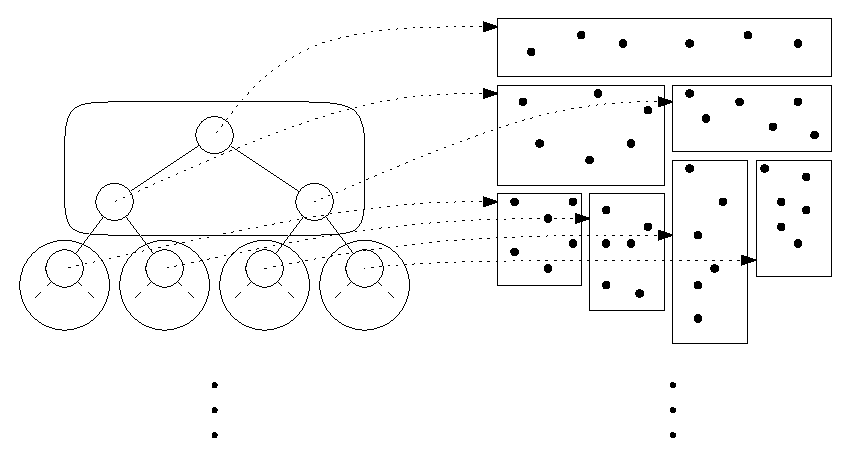
\includegraphics[width=\textwidth]{../figures/icking_external_pst}
	\caption{Illustration of the solution of Icking et al. Blocked B-tree with pointers to full buckets of data points.}
	\label{fig:icking_external_pst}
\end{figure}

Kanellakis et al. presents a linear space partially dynamic solution in~\cite{Kanellakis1996589}. The data structure answers three-sided queries in $\mathcal{O}(\log_B N + \nicefrac{K}{B} + \log_2 B)$ I/O's and supports inserts in $\mathcal{O}(\log_B N + (\log^2_B \nicefrac{N}{B})$ I/O's. The result is fairly involved and is unlikely to perform well in any practical manner. We will omit the full details and only present the overall ideas. As a first step all points are shifted such that they lie above the line $y = x$. The basic building block of the data structure is the \textit{metablock tree}; a B-ary tree of \textit{metablocks}, each of which represents $B^2$ data points. The root represents the $B^2$ data points with the largest $y$-values. The remaining $N - B^2$ data points are divided into $B$ groups of $(N - B^2)/B$ data points each based on the $x$-coordinates. The first group contains the $(N - B^2)/B$ data points with the smallest $x$-values and so on. A recursive tree of the exact same type is constructed for each such group of data points. This process continues until a group has at most $B^2$ data points and can fit into a single metablock. Please refer to figure~\ref{fig:kanellakis_metablock_tree} for an illustration of a metablock tree.

\begin{figure}[h]
	\centering
		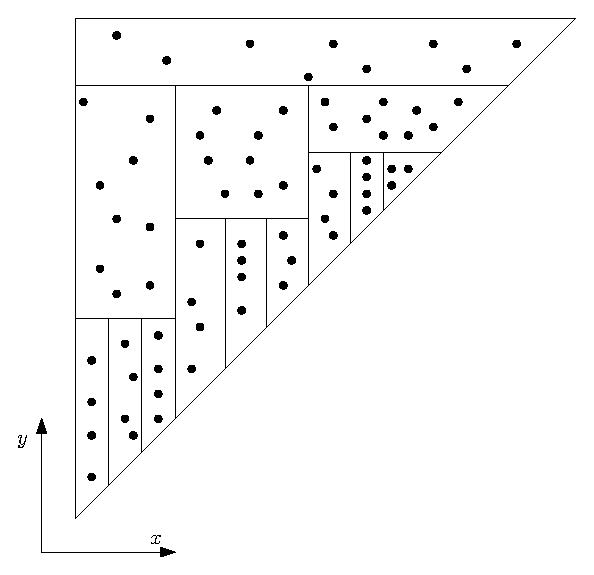
\includegraphics[width=0.5\textwidth]{../figures/kanellakis_metablock_tree}
	\caption{A metablock tree for $B=3$ and $n=70$. All data points lie above the line $y=x$. Each region represents a metablock. The root is at the top. Note that each nonleaf metablock contains $B^2 = 9$ data points.}
	\label{fig:kanellakis_metablock_tree}
\end{figure}

Points from each $metablock$ are copied into new blocks that both vertically and horizontally oriented as depicted in figure~\ref{fig:kanellakis_vertical_horizontally_oriented_blocks}. 

\begin{figure}[h]
	\centering
		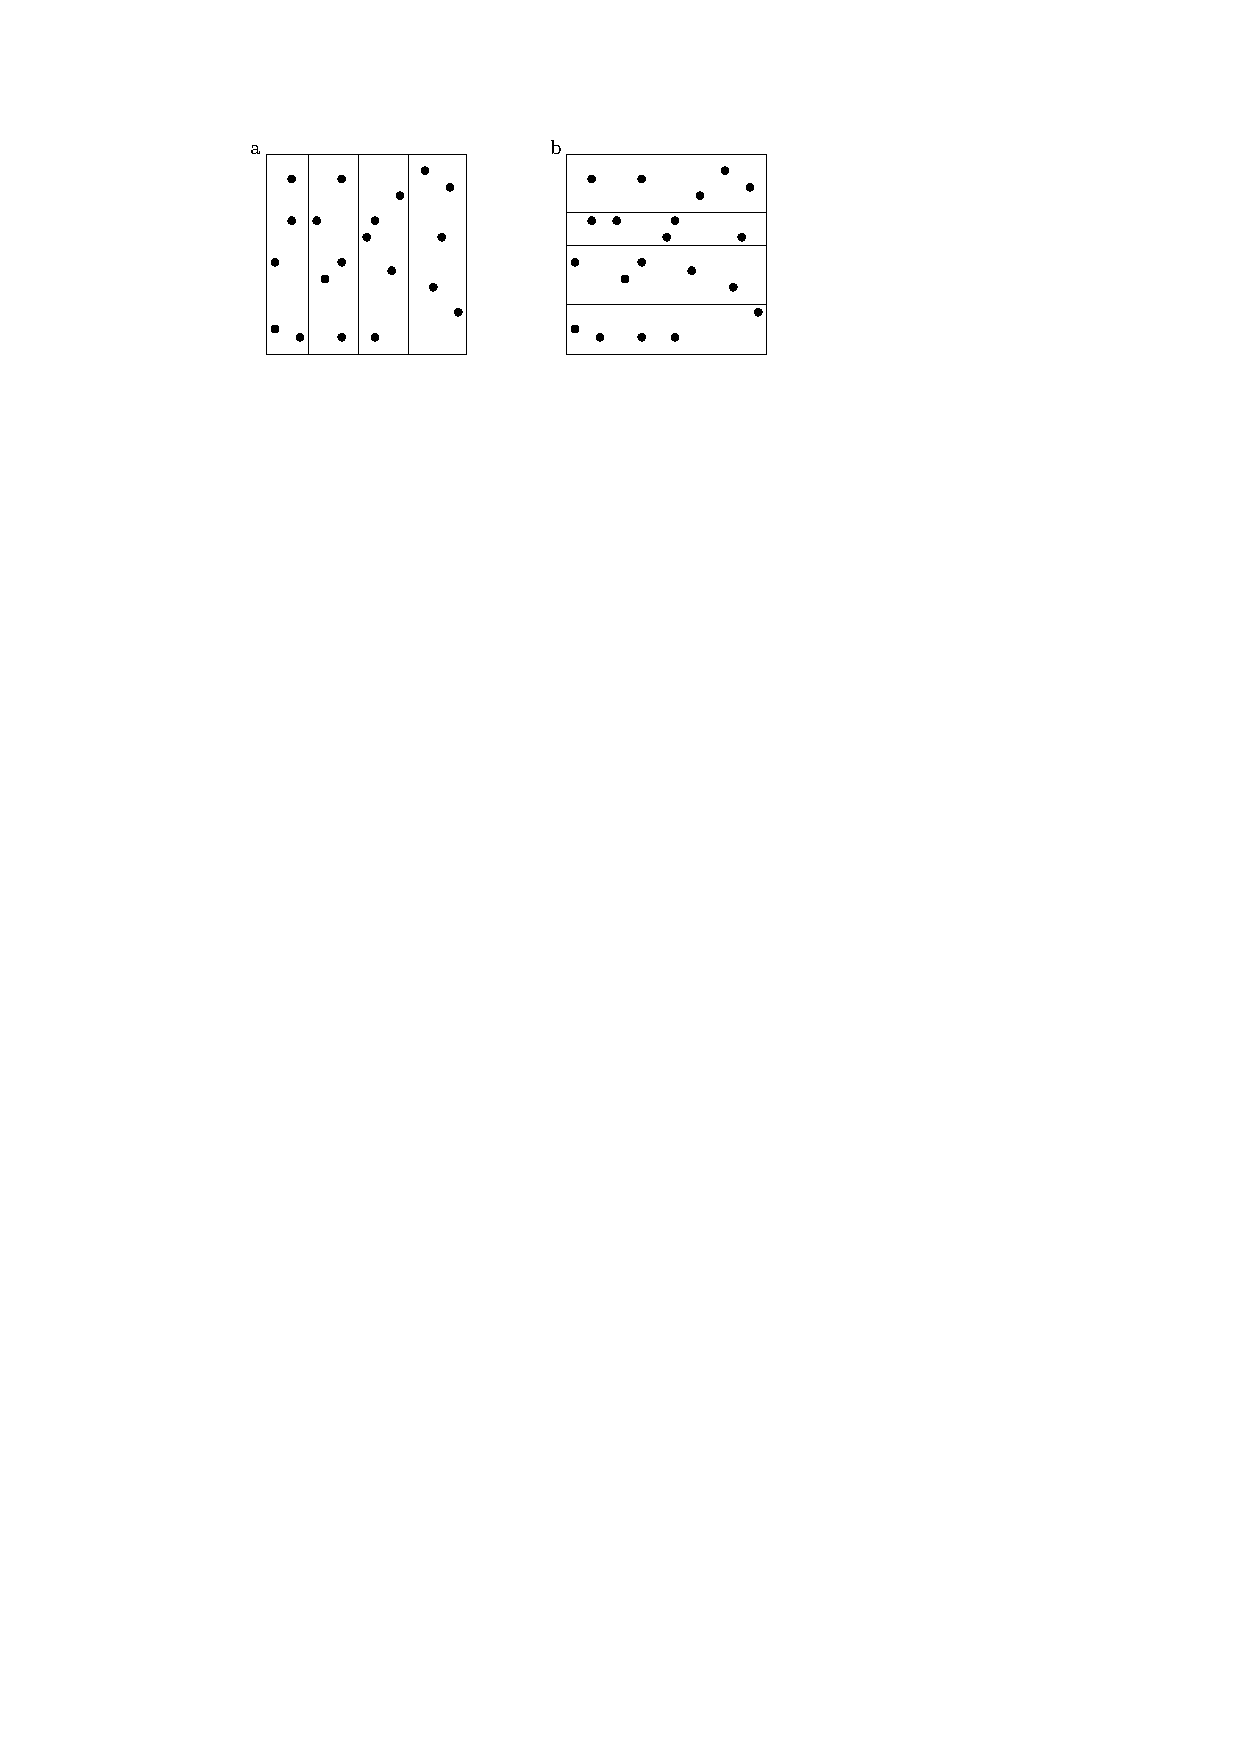
\includegraphics[width=0.5\textwidth]{../figures/kanellakis_vertical_horizontally_oriented_blocks}
	\caption{Vertically and horizontally oriented blockings of data points. Each rectangle represents a block: (a) vertically oriented; (b) horizontally oriented.}
	\label{fig:kanellakis_vertical_horizontally_oriented_blocks}
\end{figure}

Finally, each metablock $M$ contains pointers to B blocks that represents the set TS(M) that is obtained by examining the left siblings of $M$ and taking the $B^2$ largest points according to the $y$-value. Depending on how the query spans the metablock tree we can query the auxiliary data structures in such a way that we can achieve the promised $\mathcal{O}(\log_B N + \nicefrac{K}{B} + log_2 B)$ I/O's. The five different query cases are depicted in figure~\ref{fig:kanellakis_queries}.

\begin{figure}[h]
	\centering
		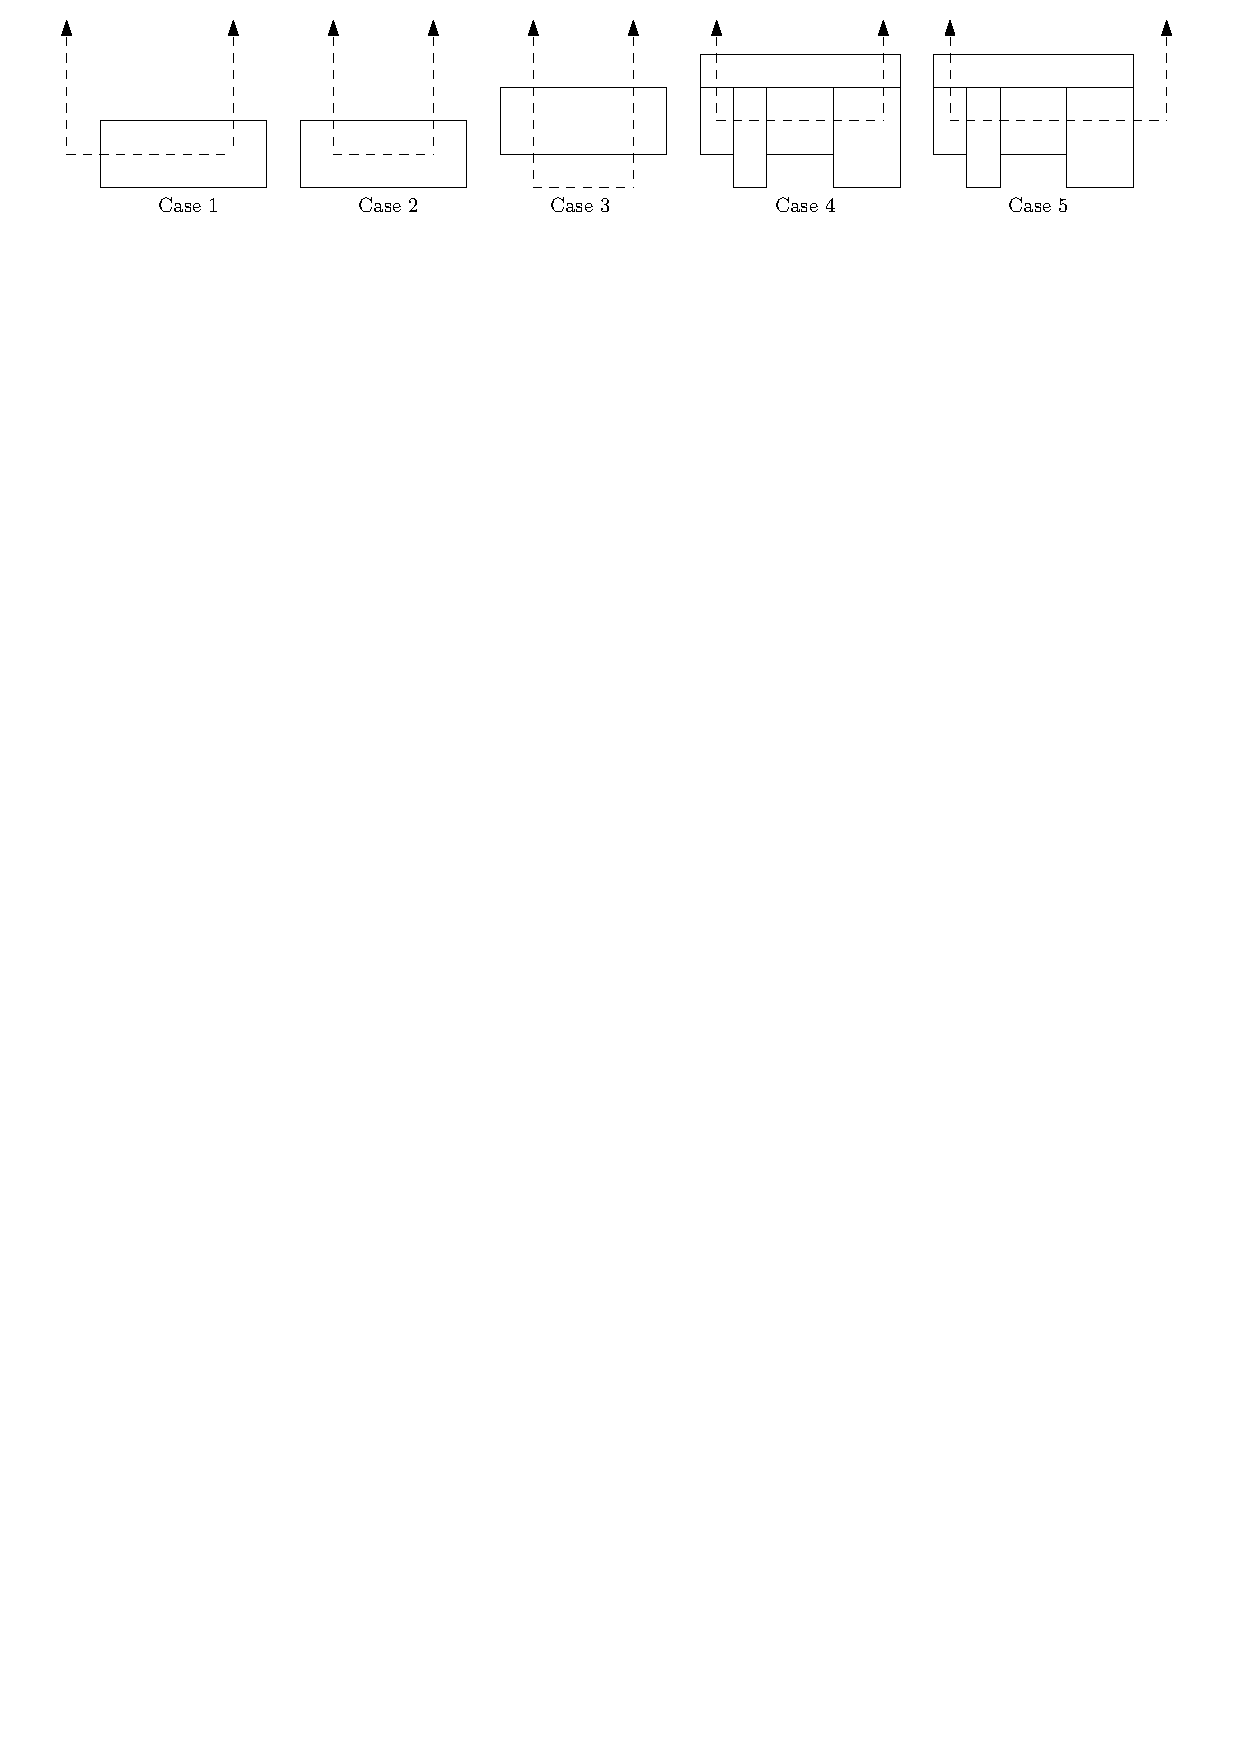
\includegraphics[width=1\textwidth]{../figures/kanellakis_queries}
	\caption{The three-sided queries can span the metablock tree in five different ways.}
	\label{fig:kanellakis_queries}
\end{figure}

Ramaswamy and Subramanian presents a suboptimal space data structure that answers queries with an optimal query bound in \cite{Ramaswamy:1994:PCT:182591.182595}. They use the same basic blocked B-tree with pointers to full buckets of data points as introduced by Icking et al.~\cite{Icking1988} and illustrated in figure~\ref{fig:icking_external_pst}. In addition they introduce the idea of \textit{path caching} that we will explain shortly. It can trivially be seen that by using a B-tree we are able to answer 2-sided queries in $\mathcal{O}(\log N + \nicefrac{K}{B})$ I/O's by classifying points inside the query into four categories as follows:

\begin{itemize}
	\item \textit{Corner}: this is the node whose region contains the corner of the query.
	\item \textit{Ancestors of the corner}: These are nodes whose regions are cut by the left side of the query. There can be at most $\mathcal{O}(\log N)$ such nodes.
	\item \textit{Right siblings of the corner and the ancestors}: these are nodes whose parents' regions are cut by the left side of the query. There can be at most $ \mathcal{O}(\log N)$ such nodes.
	\item \textit{Descendants of right siblings}: there can be an unbounded number of them, but for every such node, its parent's region has to be completely contained inside the query. That pays for the cost of looking into these nodes. That is, for every $J$ descendant blocks that are partially cut the query, the will be at least $\nicefrac{J}{2}$ blocks that lie completely inside the query. 

\end{itemize} 
 
Please refer to figure~\ref{fig:ramaswamy_query} for an illustration of the categories. \\

\begin{figure}[h]
	\centering
		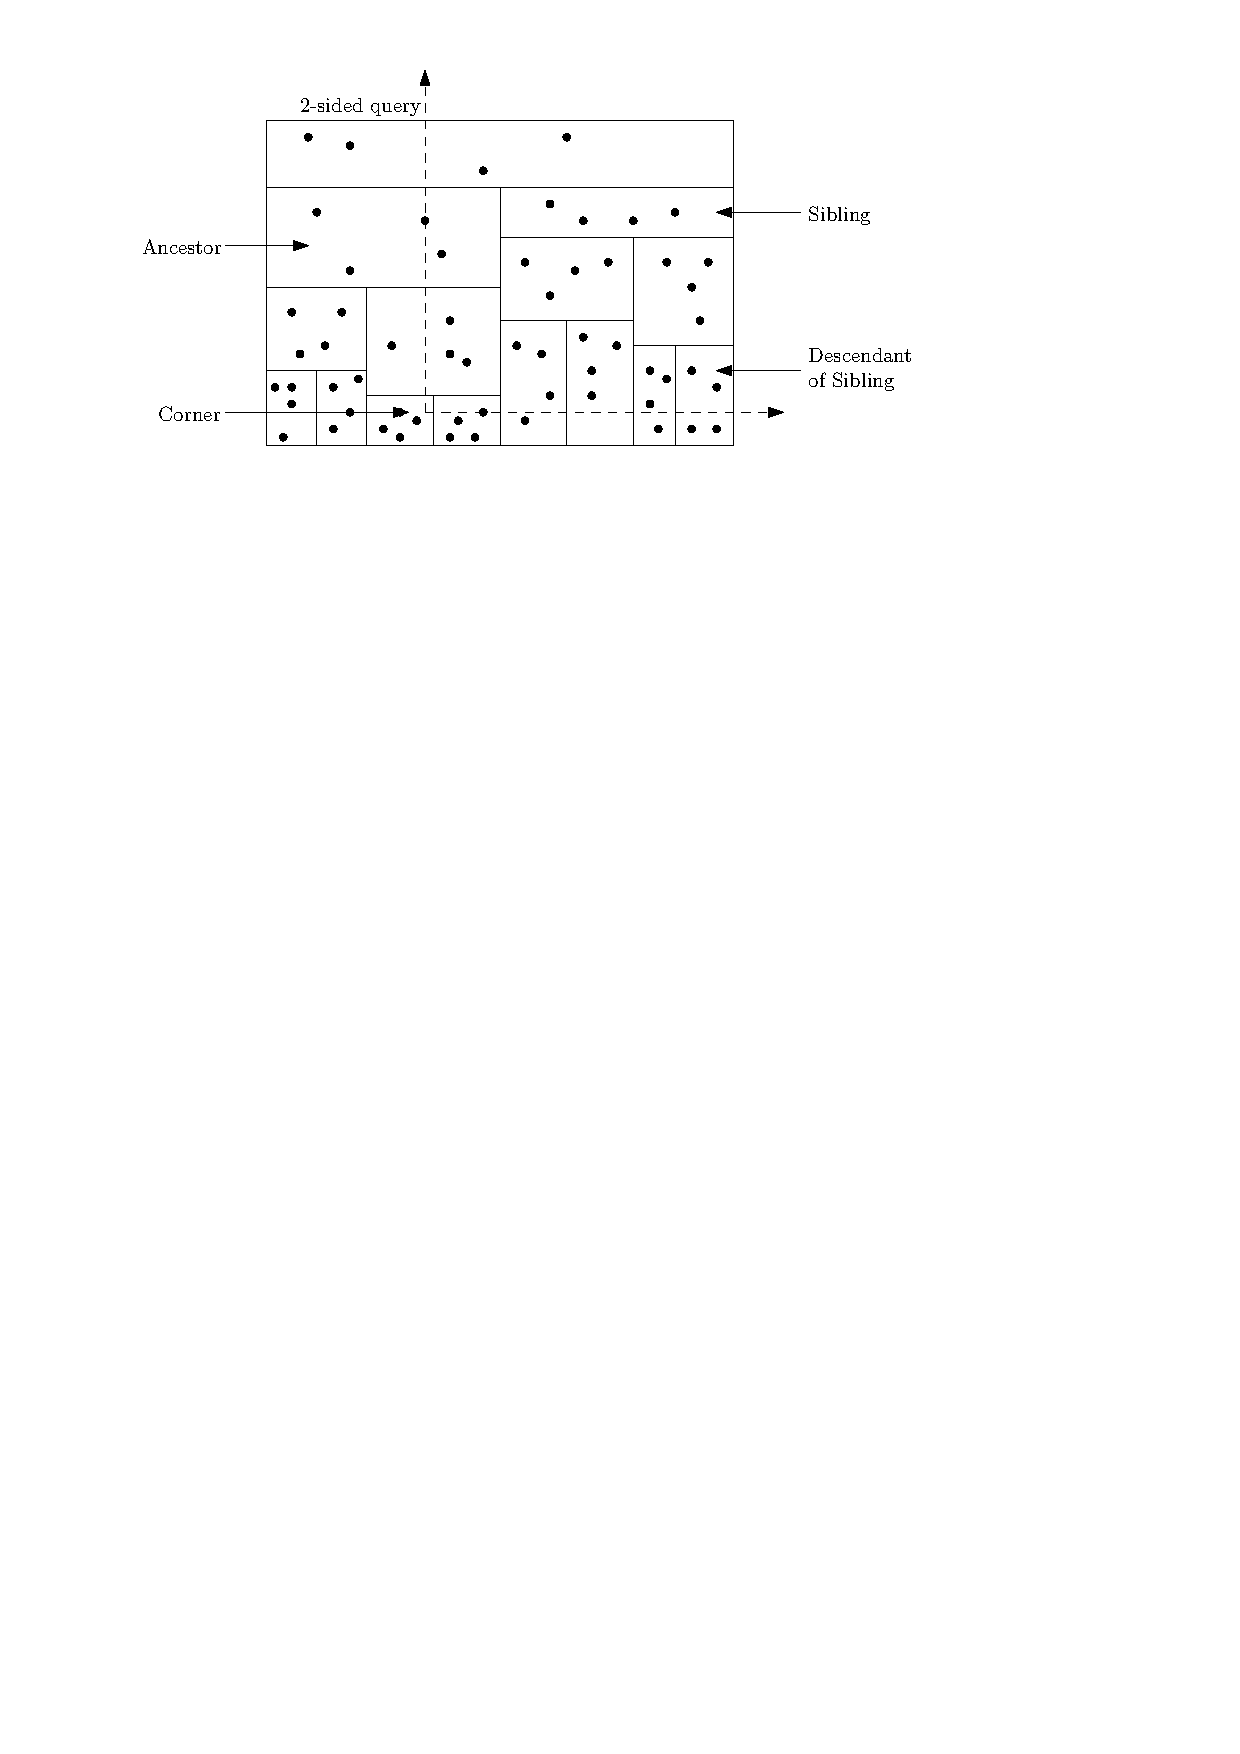
\includegraphics[width=0.9\textwidth]{../figures/ramaswamy_query}
	\caption{Binary tree implementation of Priority Search Tree in secondary memory showing a corner, ancestor sibling and sibling's descendant. Here, B is 4.}
	\label{fig:ramaswamy_query}
\end{figure}

Querying is done by locating the nodes intersecting the left side of the query using the B-tree. Points from the nodes are reported by examining the associated buckets. Next, right siblings of the nodes and their descendants are examined in a top-down fashion until the bottom boundary of the query is crossed. It is crucial to note that the corner, ancestor, and sibling nodes can cause wasteful I/O's. Thus there are $\mathcal{O}(\log N)$ wasteful nodes as the every parent of a visited node would have contributed an useful I/O. From this analysis we can conclude that we can answer 2-sided queries in $\mathcal{O}(\log N + \nicefrac{K}{B})$ I/O's. Now, we are able to avoid the wasteful I/O's by caching the data in the ancestor and sibling nodes. By associating two caches with the corner that contain all data in the siblings sorted by $x$-coordinate and $y$-coordinate respectively, we are able to answer queries in $\log_B n + \nicefrac{K}{B}$ I/O's by simply locating the corner in $\mathcal{O}(\log_B N)$ I/O's and report using the cache. The storage use is $\mathcal{O}(\nicefrac{N}{B} \log N)$ disk blocks of size $B$ each. The idea can be extended to handle 3-sided queries by adding additional caches that cover point sets sorted from right to left. This gives a space usage of $\mathcal{O}(\nicefrac{N}{B} \log^2 N)$. 

Ramaswamy and Subramanian continues their work and brings down the space usage in~\cite{Subramanian:1995:PTN:313651.313769}. This done by building a search tree that divides the points into regions of size $B \log B$ instead of $B$ giving a total of $\nicefrac{N}{B} \log B$ regions. Now a slightly modified caching scheme is used with an addition secondary level structure for each region giving a total space usage of $\mathcal{O}(\nicefrac{N}{B} \log \log B)$. Reusing this idea in a multilevel scheme brings down the data structure to a $\mathcal{O}(\nicefrac{N}{B} \log B \log^* B)$ space solution that answers queries in $\mathcal{O}(\log_B + \nicefrac{K}{B} + \mathcal{IL}^*(B))$, where $\mathcal{IL^*}(x)$ denotes the number of times $\log^*$ must be applied before the result becomes $\leq 2$.

Arge et al. presented the first optimal linear space dynamic data structure in~\cite{arge_samoladas_vitter_1999}. The data structure supports queries using $\mathcal{O}(\log_B N + \nicefrac{K}{B})$ I/O's and updates using $\mathcal{O}(\log_B N)$ I/O's. Please refer to chapter~\ref{chp:arge_pst} for a detailed description of the solution.

Brodal~\cite{DBLP:journals/corr/Brodal15} introduced an amortized solution that improves the update bound of~\cite{arge_samoladas_vitter_1999} by a factor $\epsilon B^{1-\epsilon}$ and query bound by a factor $\epsilon^{-1}$ by adopting ideas of the buffer trees of Arge~\cite{Arge:1995:BTN:645930.672850} to the external memory priority search tree of Arge~\cite{arge_samoladas_vitter_1999}. The solution is presented in detail in chapter~\ref{chp:epst}.

Please refer to table~\ref{tbl:related_work_summary} for a summary of the results.

\todo{isn't epsilon between 0 and 0.5?}

\begin{table}[h]
\centering
\caption{Previous dynamic external-memory three-sided range reporting data structures. All query bounds except for~\cite{Subramanian:1995:PTN:313651.313769} are optimal. Amortized bounds are marked \textdagger, and $\epsilon$ is satisfying $0 < \epsilon < 1$. All data structures requires $\mathcal{O}(\nicefrac{N}{B})$ space, except for~\cite{Ramaswamy:1994:PCT:182591.182595} requiring space $\mathcal{O}(\nicefrac{N}{B} \log_2 B \log \log B)$. $\mathcal{IL^*}(x)$ denotes the number of times $\log^*$ must be applied before the result becomes $\leq 2$}
\label{tbl:related_work_summary}
\centerline{
\begin{tabular}{llll}
\multicolumn{1}{c}{\small{Reference}} & \multicolumn{1}{c}{\small{Update}} & \multicolumn{1}{c}{\small{Query}} & \multicolumn{1}{c}{\small{Construction}} \\ \hline
\multicolumn{1}{c}{\small{\cite{Ramaswamy:1994:PCT:182591.182595}}} & \multicolumn{1}{c}{\small{$\mathcal{O}(\log N \log B)^{\text{\textdagger}}$}} & \multicolumn{1}{c}{\small{$\mathcal{O}(\log_B N + K/B)$}} &  \\
\multicolumn{1}{c}{\small{\cite{Subramanian:1995:PTN:313651.313769}}} & \multicolumn{1}{c}{\small{$\mathcal{O}(\log_B N + (\log_B N)^2 / B)^{\text{\textdagger}}$}} & \multicolumn{1}{c}{\small{$\mathcal{O}(\log_B N + K/B + \mathcal{IL}^*(B))$}} & \\
\multicolumn{1}{c}{\small{\cite{Arge:1995:BTN:645930.672850}}} & \multicolumn{1}{c}{\small{$\mathcal{O}(\log_B N)$}} & \multicolumn{1}{c}{\small{$\mathcal{O}(\log_B N + K/B)$}} & \\
\multicolumn{1}{c}{\small{\cite{DBLP:journals/corr/Brodal15}}} & \multicolumn{1}{c}{\small{$\mathcal{O}(\frac{1}{\epsilon B^{1-\epsilon}} \log_B N)^{\text{\textdagger}}$}} & \multicolumn{1}{c}{\small{$\mathcal{O}(\frac{1}{\epsilon}\log_B N + K/B)^{\text{\textdagger}}$}} & \multicolumn{1}{c}{\small{$\mathcal{O}(\text{Sort}(N))$}} \\ \hline
\end{tabular}
}
\end{table}

\todo{Add description of buffer tree as this structure is what Brodal is based upon}

\section{Lower bounds}	
Solving the problem of three sided range queries is very closely related to that of the 1D-dictionary. Any solution that solves the three sided range query problem can solve the 1D-dictionary problem by testing membership of an element $(x,y)$ by reporting all points in the range $\left[x,x\right] \times \left[y, \infty\right]$. By reduction we must have that the lower bounds of the 1D-dictionary problem also applies to that of three sided range queries.

The 1D-dictionary problem has been a popular topic in the case of internal memory. It has been proved by a simply adversary argument that a query can be forced to cost $\log_2 N$ comparisons no matter the cost of updates, and more generally it has been proved that if an insertion perform at most $\mathcal{O}(k)$ comparisons then queries can be forced to cost at most $\max\left\lbrace \log_2 N, N/2^{\Theta(k)}\right\rbrace$ comparisons~\cite{Borodin81efficientsearching}.

There has also been much work on the lower bounds of the 1D-dictionary problem in external memory.

We here give an adversary argument which shows that for any dictionary storing $N$ elements, there exists a query requiring at least $\log_B \frac{N}{M} - \mathcal{O}(1)$ I/O's, i.e. a lower bound for queries in external memory dictionaries. The argument goes like this: 

Assume that we are at a position in our dictionary where the elements that can still be equal to our query are denoted \textit{candidate elements}. These elements form a consecutive subsequence in the partial ordering of the $N$ elements in the dictionary.
Initially we can have at most $M$ elements in internal memory. The adversary will now select a partial ordering of these $M$ elements, i.e. select answers to each comparison between these $M$ elements, such that there are at least $\frac{N-M}{M+1} > \frac{N}{M+1}-1$ candidate elements left.
Each I/O will bring in $B$ elements. If we have $k$ candidate elements before this I/O then the adversary will choose a partial ordering such that there are at least $\frac{k-B}{B+1} > \frac{k}{B+1}-1$ candidate elements left.
An argument by induction will show that after $i$ I/O's there are at least $\frac{N}{(M+1)(B+1)^i} - 2$ candidate elements left. As a consistent answer to the member query cannot be given before we have only one candidate element left we have that $\frac{N}{(M+1)(B+1)^i} - 2 \leq 1 \Rightarrow i = \log_{B+1} \frac{N}{M} - \mathcal{O}(1)$.

As mentioned in Section~\ref{sec:prelim_b_tree} the B-tree is the external memory version of a binary search tree. The query bounds of the B-tree, $\mathcal{O}(\log_B N + K/B)$, are optimal, i.e. equal to the lower bound, but this is not the case for the update bounds.

Brodal and Fagerberg~\cite{Brodal:2003:LBE:644108.644201} studied two lower bound trade-offs between the I/O complexity of membership queries and updates. They arrive at the following theorem:
\begin{theorem}
If $N$ insertions perform at most $\delta \cdot N/B$ I/O's, for $1 \leq \delta \leq B \log_B N$ then
\begin{enumerate}
	\item There exists a query requiring at least $\log_{B+1} \frac{N}{M} - \mathcal{O}(1)$ I/O's.
	\item There exists a query requiring $N/(M\cdot (\frac{M}{B})^{\mathcal{O}(\delta)})$ I/O's for $N > M$.
	\item There exists a query requiring $\Omega(\log_{\delta \log^2 N} \frac{N}{M})$ I/O's for N > M.
\end{enumerate}
\end{theorem}

The first is essentially just the result proved by the above adversary argument saying that B-trees have an optimal query bound.

\begin{figure}
\centering
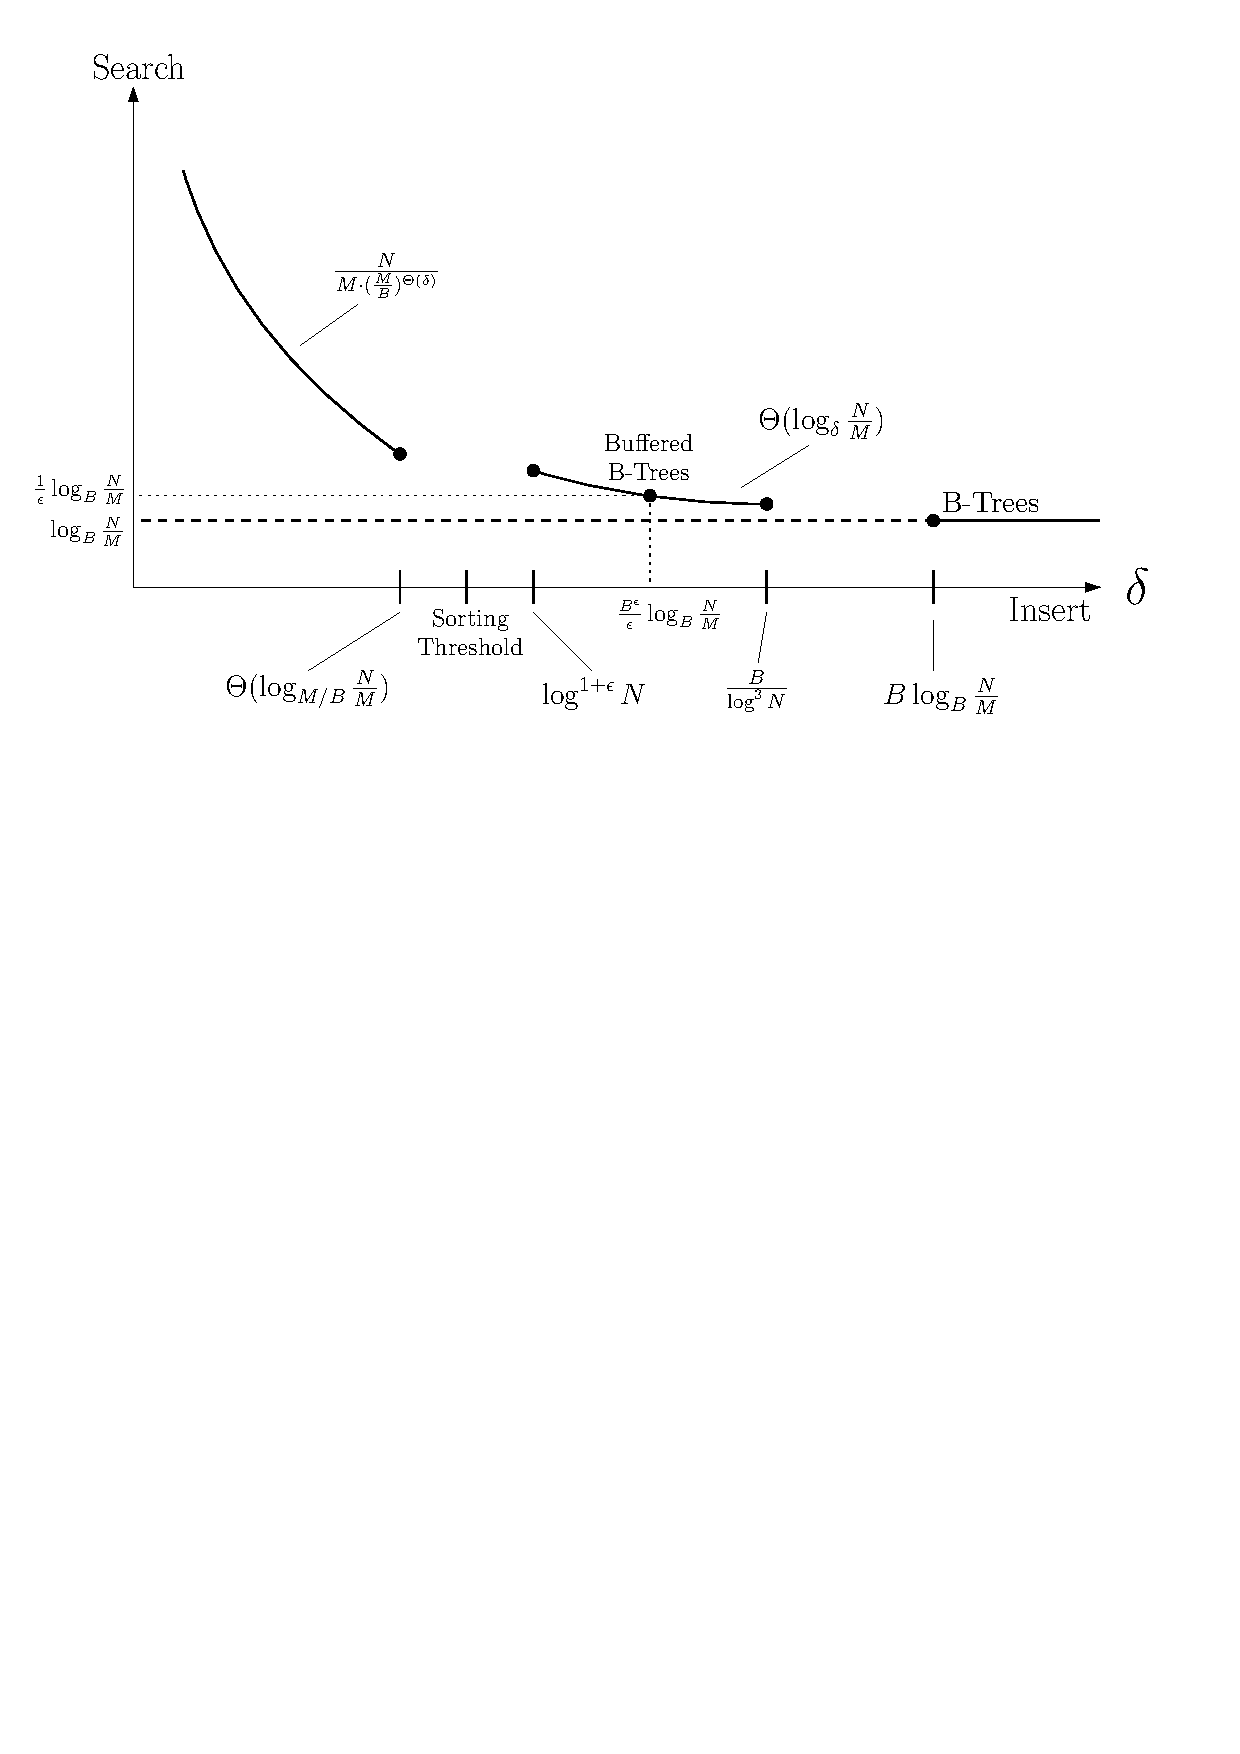
\includegraphics[width=\textwidth]{../figures/lower_bound_summary}
\caption{A summary of the results of Brodal and Fagerberg~\cite{Brodal:2003:LBE:644108.644201}. It depicts the trade-off between insert and search/query. On one end we can achieve really fast insert operations but pay the price with slow queries. In the other end we have the B-tree which query bound matches the optimal but has suboptimal insertions. No results exists for the gaps.}
\label{fig:lower_bound_summary}
\end{figure}

The results by Brodal and Fagerberg assume that points are indivisible. Iacono and P\v{a}tra\c{s}cu~\cite{Iacono:2012:UHS:2095116.2095164} looks at what happens when we do not have this assumption and are thus allowed to use hashing. They improve the update time of the buffer tree by roughly a logarithmic factor. More precisely they arrive at the following theorem:

\begin{theorem}
For any $\max\left\lbrace \log\log N, \log_M N \right\rbrace \leq \lambda \leq B$, we can solve the dictionary problem by a Las Vegas data structure with update time $t_u = \mathcal{O}(\frac{\lambda}{B})$ and query time $t_q = \mathcal{O}(\log_\lambda N)$ with high probability.
\end{theorem}

This means that in one end of the trade-off they can for $\lambda = B^\epsilon$ obtain an update time of $\mathcal{O}(1/B^{1-\epsilon})$ and query time of $\mathcal{O}(\log_B N)$. This matches the bounds of the buffer tree of Arge. In the other end of the trade-off where they are able to achieve fast updates very close to the optimal disk transfer rate of $1/B$ namely they obtain: $t_u^{\min} = \mathcal{O}(\frac{1}{B} \cdot \max\left\lbrace \log\log N, \log_M N \right\rbrace)$.

\chapter{Internal Priority Search Tree}
\label{chp:internal_pst}
In this section we present an internal memory data structure for the range reporting problem. The data structure was originally presented by McCreight~\cite{DBLP:journals/siamcomp/McCreight85} and is denoted a priority search tree. The priority search tree is basically a combination of a binary search tree on the $x$-coordinate and a heap on the $y$-coordinate. A formal definition of a priority search tree for a set of $N$ points, $P$, is as follows. We assume that all points have distinct coordinates, though this assumption can be removed by using the normal lexicographical ordering of points.

\begin{itemize}
	\item If $P = \varnothing$ then the priority search tree is an empty leaf.
	\item Otherwise, let $p_\text{max}$ be the point in the set $P$ with the largest $y$-coordinate. \\ \\
			Let $x_{\text{mid}}$ be the median of the $x$-coordinates of the remaining points. \\ \\ Now let
			$$ P_\text{below} \coloneqq \{p \in P \setminus \{p_\text{max} \} : p_x < x_\text{mid} \}\text{,}$$
			$$ P_\text{above} \coloneqq \{p \in P \setminus \{p_\text{max} \} : p_x > x_\text{mid} \}\text{.}$$
			
			The priority search tree consists of a root node $v$ where the point \\
			$p(v) \coloneqq p_{\text{max}}$ and the value $x(v) \coloneqq x_{\text{mid}}$ are stored. Furthermore,
			\begin{itemize}[label=$\bullet$]
				\item the left subtree of $v$ is a priority search tree for the set $P_{\text{below}}$.
				\item the right subtree of $v$ is a priority search tree for the set $P_{\text{above}}$.
			\end{itemize}
\end{itemize}

What is important to note is that the specific construction method allows the data structure to be indexed in two different ways. First, the tree can be searched as a binary search tree based on $x$-coordinate. Second, the tree operates as a max-heap based on $y$-coordinate. Please refer to Figure~\ref{fig:static_pst} for an illustration of a priority search tree constructed on points $P = \{A, B, C, D, E, F, G, H\}$.

\begin{figure}[h]
	\centering
	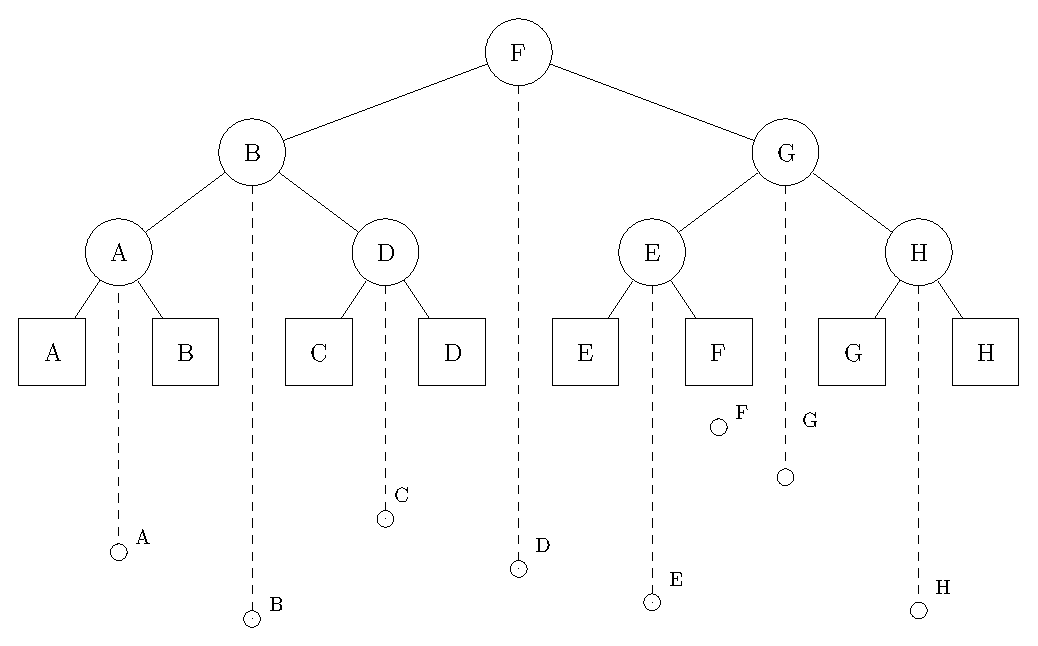
\includegraphics[scale=0.68]{../figures/internal_pst_static}
	\caption{The letter given in the node represents the $y_{\text{max}}$ stored as key, while the dashed line represents the median $x$ value stored in the node.}
	\label{fig:static_pst}
\end{figure}

\section{Three-sided Range Query}
When answering a query of the form $[x_1,x_2] \times [y,\infty]$ we begin at the root of the tree and first check the $y$-coordinate of this node against the $y$-coordinate of the baseline of the query interval. As long as the $y$-coordinate of the current node is greater than the $y$-coordinate of the horizontal segment defining the base of our three-sided range, we will continue down the tree. We can use the fact that the tree is a basic binary search tree on the $x$-coordinates to only visit the part of the tree that is within our search range. Please refer to Figure~\ref{fig:static_pst_query} for an illustration of the general query pattern.

\begin{figure}[h]
	\centering
	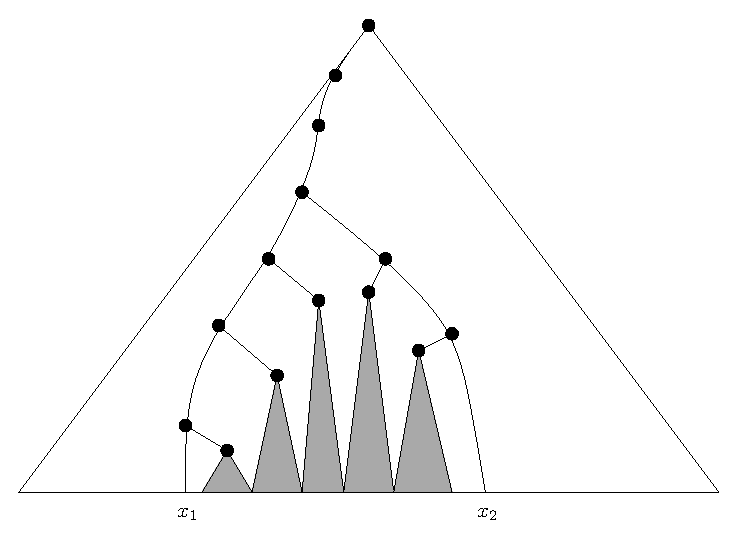
\includegraphics[scale=0.7]{../figures/internal_pst_query}
	\caption{The shaded subtrees in the figure stores only points with $x$-coordinate within the correct range. This property ensures we can search the subtrees based on $y$-coordinate only.}
	\label{fig:static_pst_query}
\end{figure}

\subsection*{Analysis}
The search operation follows two root to leaf paths each of length $\mathcal{O}(\log N)$. Using the search path and heap property of the tree we are guaranteed to only visit nodes that is actually reported when querying. This gives a total running time of $\mathcal{O}(\log N + K)$.

\section{Dynamic Priority Search Tree}
The key difference between the static solution presented by McCreight and a dynamic solution is that we always ensure that each point is placed in exactly one leaf and the order of the leaves from left to right corresponds to the order of the $x$-coordinate of the points. The internal nodes of the tree store the point with greatest $y$-coordinate represented by a leaf in the subtree of the node which is not already stored by an ancestor of this interior node. It is clear we have $N$ leaf nodes and $N-1$ internal nodes in the data structure.
Whenever we store a point in an interior node, then the leaf node which corresponds to this point is considered a \textit{placeholder} for this point. A total of $N - 1$ nodes are left as placeholders. Please refer to Figure~\ref{fig:dynamic_pst} for an illustration of a dynamic priority search tree over the points $P = \{A, B, C, D, E, F, G \}$.

\begin{figure}[h]
	\centering
	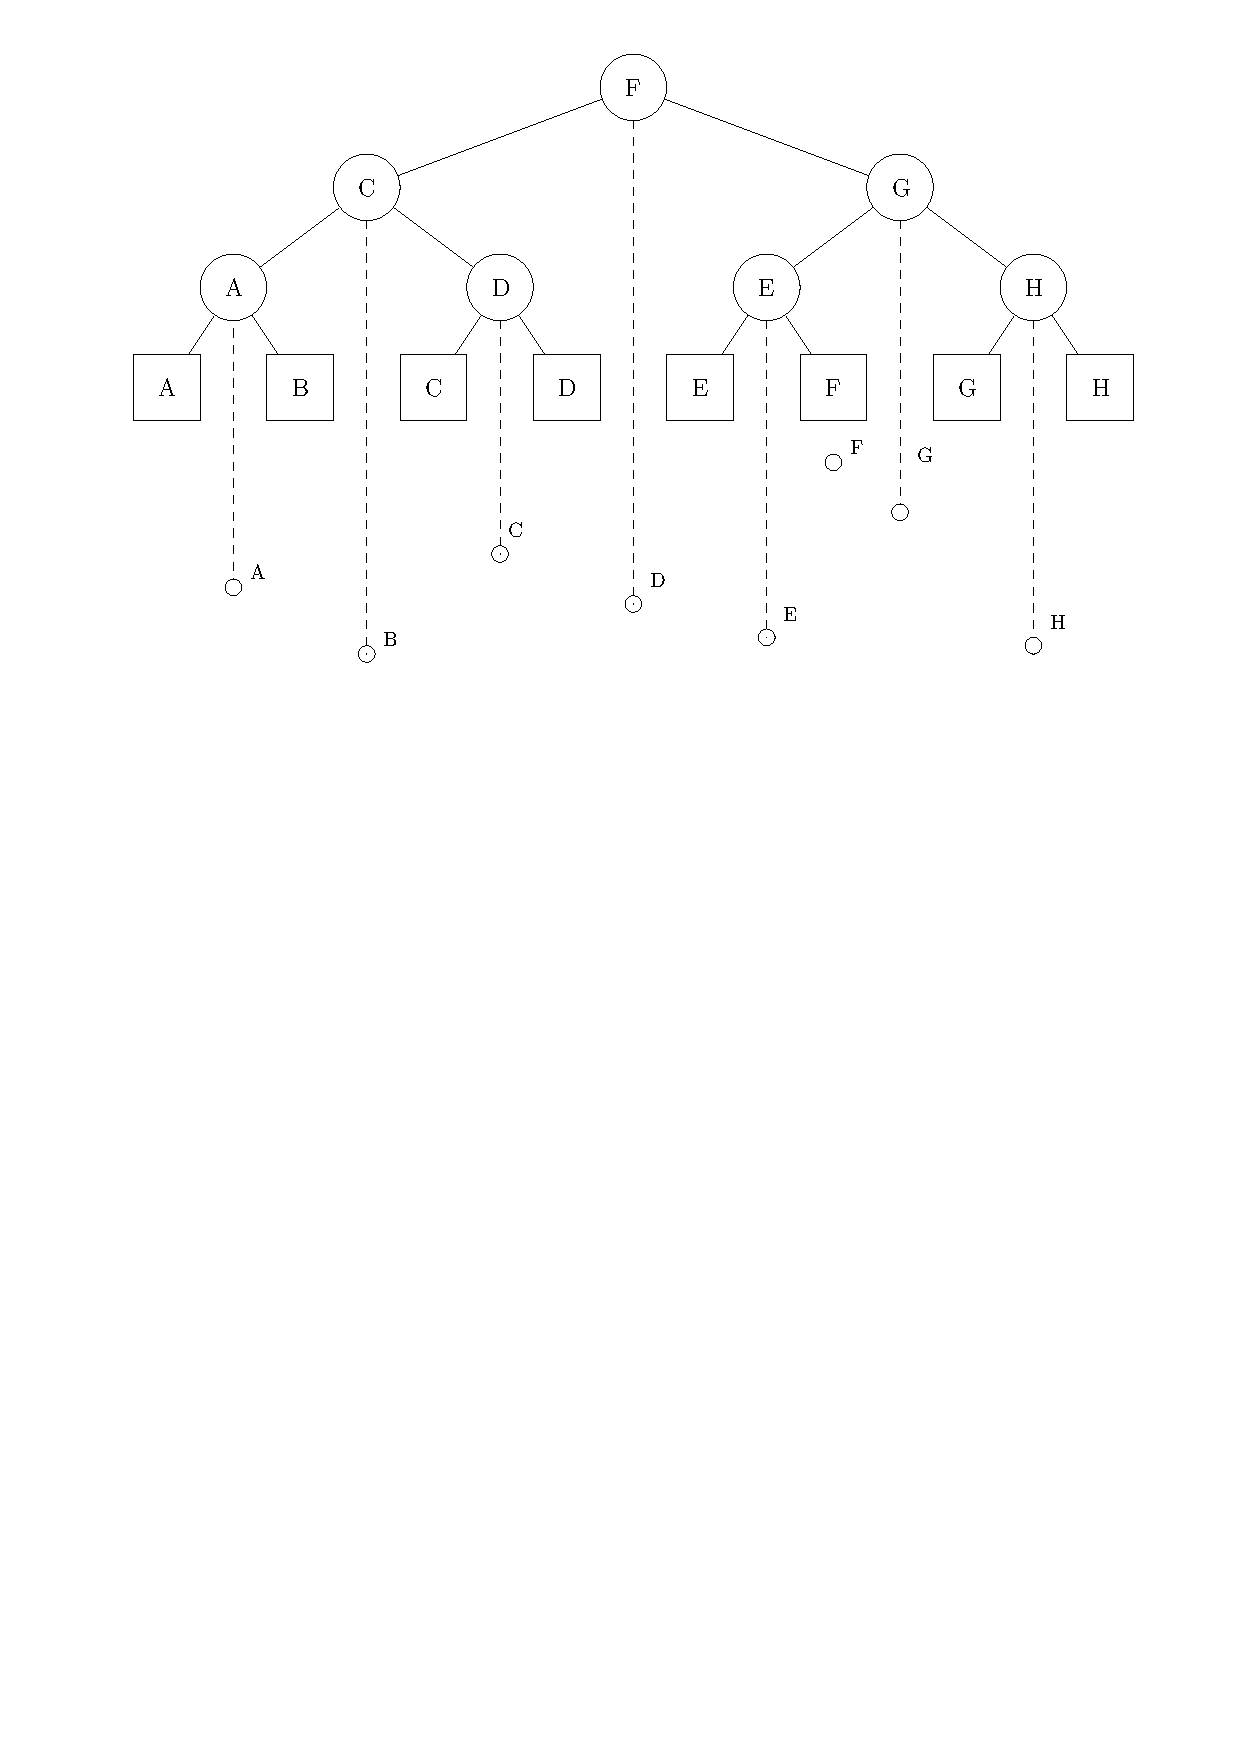
\includegraphics[scale=0.68]{../figures/internal_pst_dynamic}
	\caption{8 data points and the corresponding dynamic priority search tree. Dotted leafs are placeholders for a key higher up in the tree.}
	\label{fig:dynamic_pst}
\end{figure}

\section{Construction}
Assuming we are given a list of $x$-sorted points we can construct the dynamic priority search tree using a bottom-up construction method similar to the bottom-up construction of a heap. At the first phase of construction we associate each point with a placeholder in the priority search tree. These placeholders will become the leaf level of the data structure. Next we select pairs of placeholders and compare them to one another in terms of their $y$-coordinate. We denote the point with the highest $y$-coordinate as the winning point and the comparison between points as a tournament round. It is the winning point that will be represented by a new internal node at one level higher in the tree. Please refer to Figure~\ref{fig:dynamic_pst_construction} for an illustration of the construction of the leaf level of the data structure.
At the next level of the tree, we perform the same comparisons as before to determine which nodes will advance to the third level. At most $\nicefrac{N}{2}$ are compared at this level.

\begin{figure}[h]
	\centering
	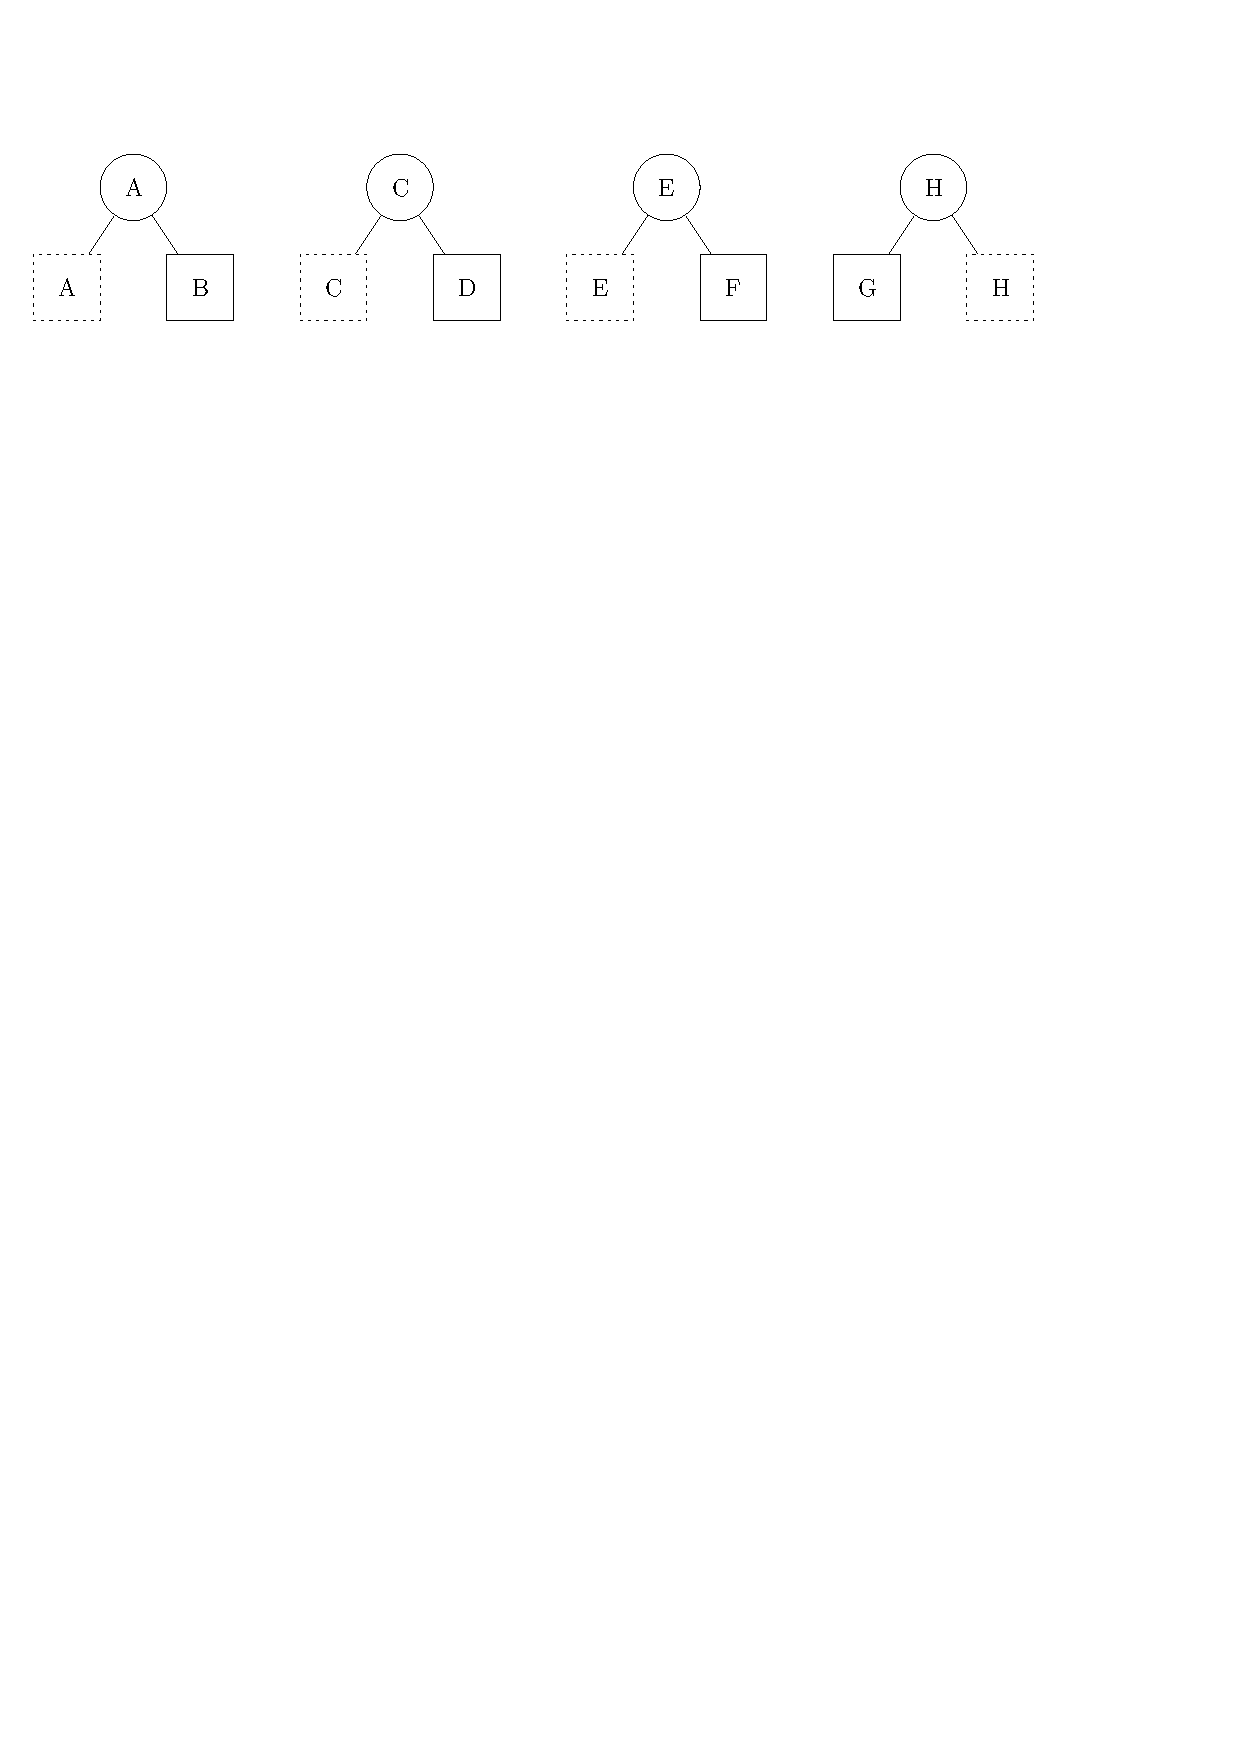
\includegraphics[scale=0.68]{../figures/internal_pst_dynamic_construction}
	\caption{The first phase of the bottom-up construction "tournament".}
	\label{fig:dynamic_pst_construction}
\end{figure}

Every tournament round will potentially leave an empty interior node behind as the wining point is moved one level up. If this occurs we have to check if any previous tournament losers are now eligible to be represented higher in the tree. We must also remember that some interior nodes in the tree may not represent any points and will thus remain empty when the construction is complete.

\subsection*{Analysis}
First, all points is inserted as leafs in the bottom layer of the data structure. The leafs counts for $\nicefrac{N}{2}$ of the total nodes in the tree. The next $N/2^2$ nodes are created at height $h = 1$ and the tournaments are played one level down. For the $i$'th step we create $N/2^i$ nodes and we will play tournaments $i$ levels down. The total steps to build the dynamic priority search tree of size $N$ is thus:

$$\sum\limits_{i=0}^{\log(N)} \frac{N}{2^{i+1}}i = \frac{N}{2} \left( \sum\limits_{i=0}^{\log(N)} i\left(\frac{1}{2}\right)^i \right) \leq \frac{N}{2} \left( \sum\limits_{i=0}^{\infty} i\left(\frac{1}{2}\right)^i \right)$$

The solution to the last summation can be found by taking the derivative of both sides of the well known geometric series:

$$ \frac{\partial}{\partial x} \left( \sum\limits_{i=0}^{\infty} x^i \right) = \frac{\partial}{\partial x} \left( \frac{1}{1-x} \right) \Rightarrow \sum_{i=1}^{\infty} ix^i = \frac{x}{(1-x)^2} $$

For $x = \frac{1}{2}$ we get

$$\frac{1/2}{(1-1/2)^2} = 2$$

Plugging this in to the above sum we get that the total number of steps to build a dynamic priority search tree on $N$ points is $\mathcal{O}(N)$.

This implies we can construct the dynamic priority search in linear time assuming we are given sorted input.

\section{Insertion}

In order to dynamically insert points into the data structure, we add a new leaf (placeholder) for the new point and perform a pushdown operation with the new point starting at the root as will be described below. We can determine where to add the new placeholder as the dynamic priority search tree is a binary search tree on the $x$-coordinate of the points. When we reach an existing leaf, we add a new internal node in place of this leaf, and make the existing leaf one of the children of this new internal node. Then we add a new leaf to the tree as the other child, and store the new point in this leaf. In order to maintain the heap order of the priority search tree we now perform a pushdown operation, where we at each step compare the $y$-coordinate of the point to be inserted with the $y$-coordinate of the point represented by the given internal node. If the $y$-coordinate of the point to be inserted is less than that of the point stored in the internal node, then we push the point to be inserted further down the tree. However, if the $y$-coordinate of the point to be inserted is greater than the $y$-coordinate of the point in the internal node, then we store the point to be inserted in this internal node, and take the point which was formerly represented by this internal node and continue the pushdown operation with this point instead.

\subsection*{Analysis}

The first step of the insertion algorithm is a binary search traversal on the $x$-coordinate of the new point. The path is of length $\mathcal{O}(\log N)$. Adding a new internal node in place of the old leaf takes a constant amount of operations. The pushdown operation follows a single root to leaf path of length $\mathcal{O}(\log N)$ and uses a constant amount of work in each node. So we conclude insertions can be done in $\mathcal{O}(\log N)$.

\section{Deletion}

When dynamically deleting a point we must locate the interior node (if any) representing the point we wish to delete. After we have removed the point from the interior of the dynamic search tree, we must replay a portion of the tournament among the points below this interior node in order to replace it. Finally we must delete the leaf which is the placeholder for the point.

\subsection*{Analysis}
Locating the interior node representing the point to be deleted can be done in $\mathcal{O}(\log N)$ using the binary search property maintained by the priority search tree. Once we have located the interior node we can remove this point in $\mathcal{O}(1)$. The deletion of the point of an interior node leaves a hole in the tree that we fill by playing tournaments following a node to leaf path of length $\mathcal{O}(\log N)$. We conclude the deletion algorithm requires $\mathcal{O}(\log N)$ per deletion.


\section{Rebalancing}
If we use the operations for dynamic updates as stated above without any measures for tree rebalancing, we could end up with a highly unbalanced tree. We fix this using global rebuilding when a linear number of updates have been performed. We can collect all points in sorted order in linear time by visiting leafs from left to right using a DFS traversal of the tree. On the collected points we now use the linear construction algorithm to rebalance the tree. Using this strategy yields a data structure that handles updates in $\mathcal{O}(\log N)$ amortized. By using a Red-Black tree as the heart of the tree we can achieve a data structure that is $\mathcal{O}(\log N)$ worst case by performing rotations to rebalance the tree.

\section{Bounds in the I/O model}
The above bounds translate directly to the I/O model as we cannot guarentee that nodes on the search path are perfectly placed in blocks, which in the worst case means that each visit to a node will equal 1 I/O.

\chapter{External Memory Priority Search Tree}
\label{chp:arge_pst}
In this chapter we present an older result on dynamic three-sided range queries due to Arge et al.~\cite{arge_samoladas_vitter_1999}.
The result by Arge et al. is a weight-balanced B-tree where each node is augmented with a bootstrapped structure for storing the top $\Theta(B^2)$ points w.r.t. the $y$-value of the subtree rooted at that node. This bootstrapped structure is described in Section~\ref{sec:child_structure} and the main data structure of Arge et al.~is described in Section~\ref{sec:arge_structure} proving Theorem~\ref{thm:arge_structure}.

\begin{theorem}
\label{thm:arge_structure}
An external memory data structure exists supporting insertion and deletion in amortized $\mathcal{O}(\log_B N/B)$ I/O's and three sided range queries in $\mathcal{O}(\log_B N/B + K/B)$ I/O's, where $N$ is the input size, and $K$ is the size of the output. The structure uses $\mathcal{O}(N/B)$ space, i.e. linear space.
\end{theorem}

\section{Dynamic 3-sided queries on $\Theta(B^2)$ points}
\label{sec:child_structure}
In this section we describe a data structure that supports the operations stated in Theorem~\ref{thm:child_structure}.
\begin{theorem}
\label{thm:child_structure}
There exists a dynamic data structure for storing $\mathcal{O}(B^{1+\epsilon})$ two dimensional points, $0 \leq \epsilon \leq 1$.
Insertion and deletion of $s$ points requires amortized $\mathcal{O}(1+\nicefrac{s}{B^{1-\epsilon}})$ I/O's.
The data structure supports reporting all points inside a query range of the form $[x_1,x_2] \times [y,\infty]$ in $\mathcal{O}(1+\nicefrac{K}{B})$ I/O's.
The structure uses linear space.
Finally the structure can be constructed using $\mathcal{O}(B^{1+\epsilon} / B)$ I/O's given a x-sorted set of $B^{1+\epsilon}$ points.
\end{theorem}

The structure consists of a static structure $\mathcal{L}$ storing $\mathcal{O}(B^{1+\epsilon})$ points and two buffers $\mathcal{I}$ and $\mathcal{D}$ storing at most $B$ points. $\mathcal{I}$ and $\mathcal{D}$ are initially empty and store delayed insertions and deletions, respectively. A point can appear in either $\mathcal{I}$ or $\mathcal{D}$ but not both as they cancel each other out.

Let $L$ be the points stored in $\mathcal{L}$ and let $\ell = \lceil \nicefrac{\vert L \vert}{B}\rceil$, then $\mathcal{L}$ consists of $2\ell-1$ blocks of $B$ points in each block. The points in $L$ are first partitioned into blocks $b_1,\dots,b_\ell$ sorted by $x$-value. The last block may have size less than $B$.

\begin{figure}[h]
	\centering
	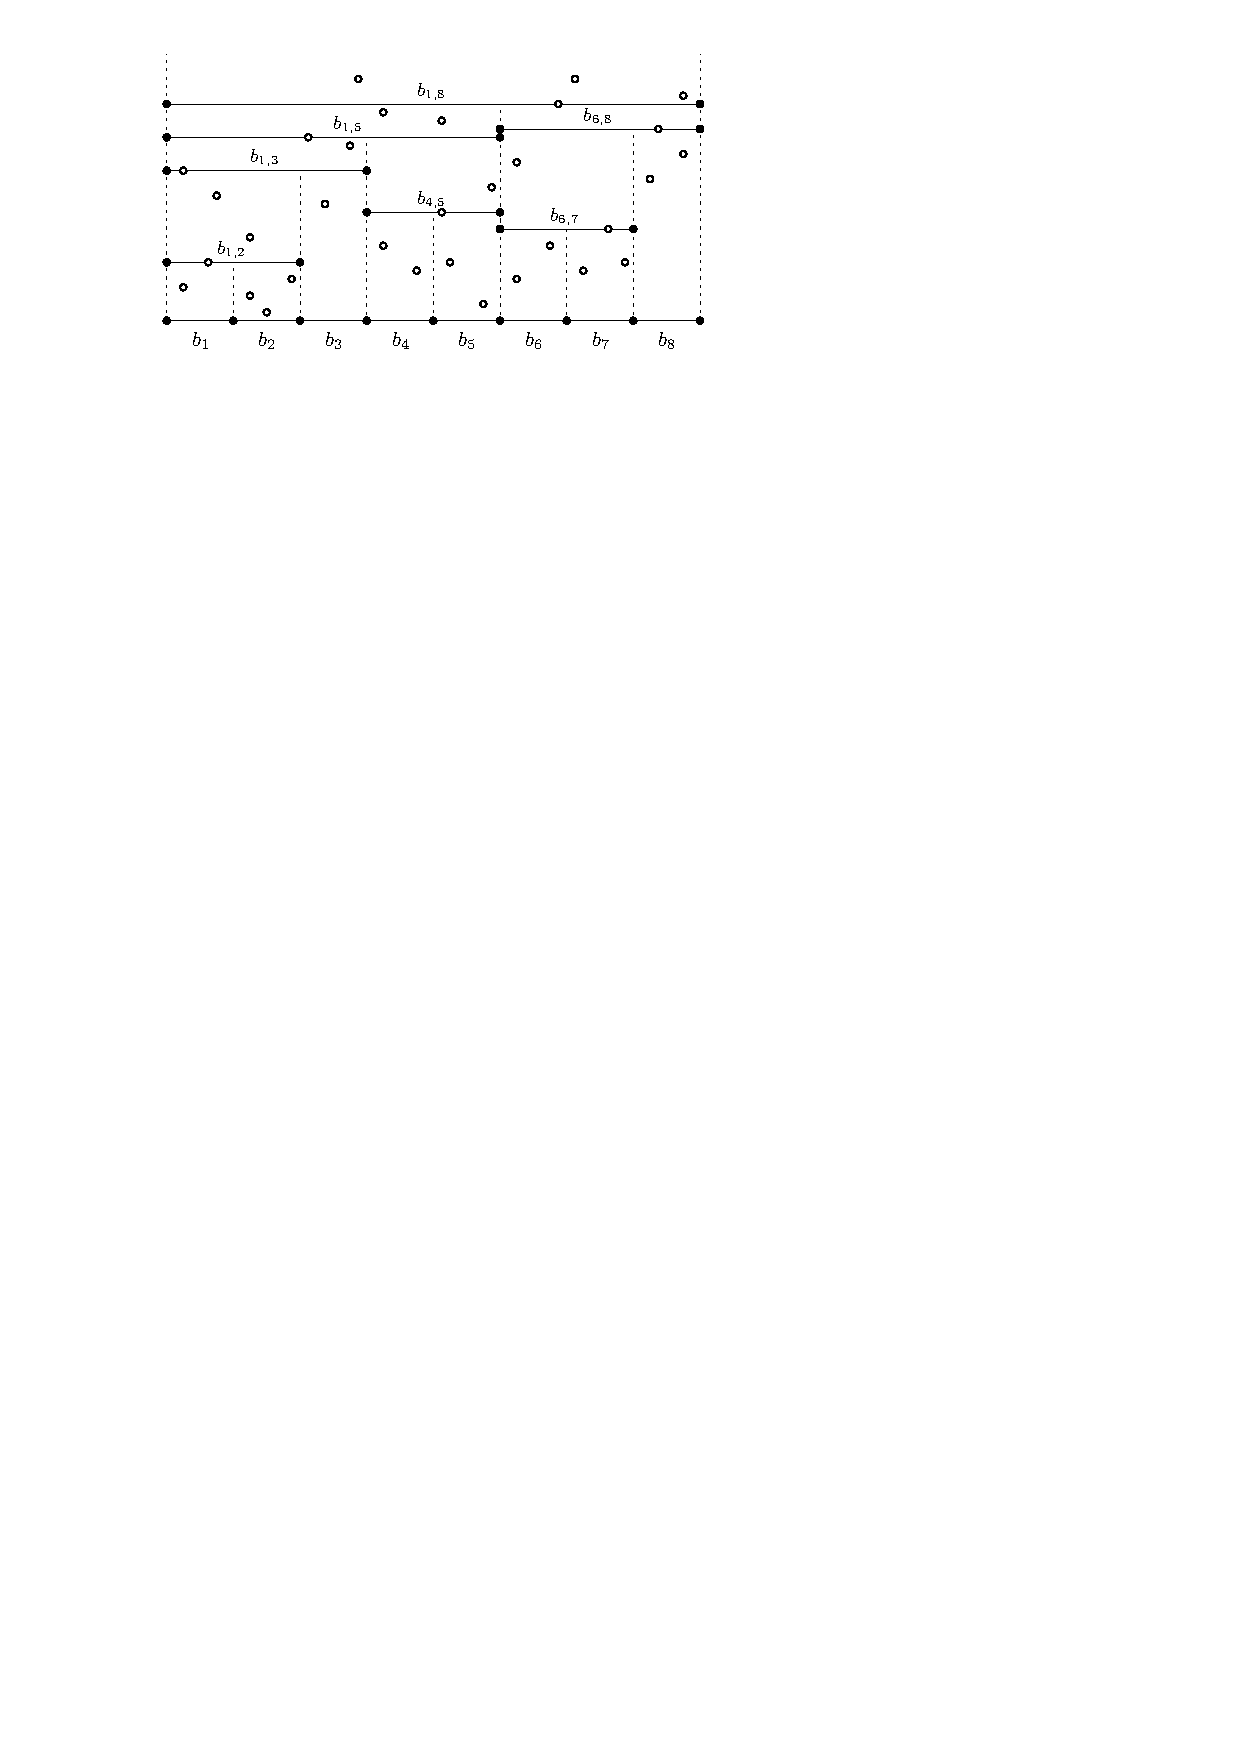
\includegraphics[scale=1]{../figures/sweep-line}
	\caption{The structure for $B=4$. The points are represented by white nodes. The sweep line has merged blocks $b_1$ and $b_2$ at the point where the blocks contain $4$ points on or above the line. This is represented by a line segment with black endpoints and the $b_{1,2}$ label. The same goes for the other merged blocks created.}
	\label{fig:sweep-line}
\end{figure}

\textbf{To construct} blocks $b_{\ell+1},\dots,b_{2\ell}$ we make a vertical sweep over the points in increasing $y$-order. When the sweep line reaches a point in a block $b_i$ that together with an adjacent block, i.e. either $b_{i-1}$ or $b_{i+1}$, contains exactly $B$ points on or above the sweep line, we replace the two blocks by a single block containing the $B$ points on or above the sweep line.  The merged block is denoted $b_{i,j}$ if it contains points from the initial blocks in the range from $i$ to $j$. The two merged blocks are then excluded from the sweep line and the newly created merged block continues in the sweep line. Every merge of adjacent blocks causes the sweep line to intersect one block less resulting in at most $\ell-1$ blocks being created from the sweep.

A catalog structure stores in $\mathcal{O}(1)$ disk blocks a reference to each of the $2\ell-1$ blocks. For block $b_i$ we store the minimum and maximum $x$-values for the points contained in the block. For a merged block $b_{i,j}$ we store the interval $\left[ i,j\right]$ and the minimum $y$-value of the points in the block. This minimum $y$-value is also the point where the sweep line created the block $b_{i,j}$.

%TODO maybe argue that L uses \mathcal{O}(B^{1+\epsilon}) blocks

%%%%%%%%%%%%%
% UPDATES %%%
%%%%%%%%%%%%%
\textbf{Insertions and deletions} are stored in $\mathcal{I}$ and $\mathcal{D}$ respectively. When a point is inserted in $\mathcal{I}$ or $\mathcal{D}$ we make sure to remove any existing occurrence of the point in $\mathcal{I}$ and $\mathcal{D}$ such that the new update overrides any previous updates. Whenever $\mathcal{I}$ or $\mathcal{D}$ overflows, i.e. $\vert \mathcal{I} \vert > B$ or $\vert \mathcal{D} \vert > B$, the stored updates are applied to the set of points in $\mathcal{L}$. This is done by scanning $L$ in increasing $x$-order while applying insertions and deletions, i.e. for each point in $L$ we check whether we should insert a new point from $\mathcal{I}$ before it or if the point should be deleted. This process results in a new set of points $L'$ which once again is partitioned into blocks $b_1,\dots,b_{\ell'}$ and a vertical sweep similar to the previously described sweep is performed to rebuild the merged blocks and catalog.
This reconstruction is done in $\mathcal{O}(\ell')$ I/O's. As $\ell' = \lceil \nicefrac{\vert L \vert}{B}\rceil$ it requires $\mathcal{O}(\lceil \nicefrac{\vert L \vert}{B}\rceil) = \mathcal{O}(B^\epsilon)$ I/O's to rebuild $\mathcal{L}$. If we amortize this cost over the $>B$ updates that caused the overflow the cost becomes $\mathcal{O}\left(\frac{B^\epsilon}{B}\right) = \mathcal{O}\left(\nicefrac{1}{B^{1-\epsilon}}\right)$ amortized I/O's per delayed update.

%%%%%%%%%%%%%
% QUERIES %%%
%%%%%%%%%%%%%
\textbf{Queries} are of the form $[x_1,x_2] \times [y,\infty]$ and can be answered by scanning the catalog to find the blocks intersected by the sweep when it was at $y$. This corresponds directly to the $t$ line segments immediately below the line segment imposed by the bottom of the query range. These blocks will contain a superset of the points contained in our query.

\begin{figure}[h]
	\centering
	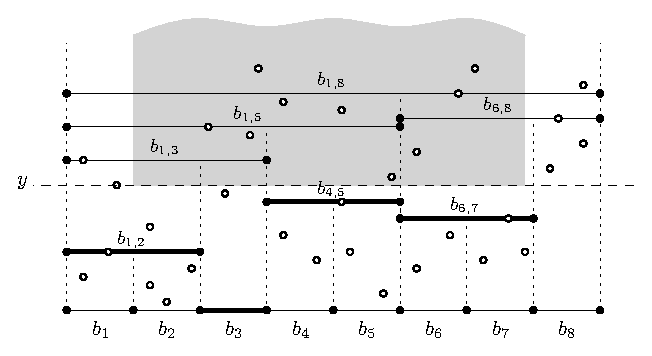
\includegraphics[scale=1]{../figures/sweep-line-with-query}
	\caption{The grey area is our query and we should report the points within. This is done by finding the fat line segments which is the segments just below the sweep line at $y$. The segments can be found using the catalog and the blocks can be scanned and points reported in $\mathcal{O}(1+\nicefrac{K}{B})$.}
	\label{fig:sweep-line-query}
\end{figure}

We know from construction that the blocks intersected contains $B$ points on or above the sweep line. The left most and right most of these blocks are not necessarily fully contained in the query range and do not necessarily contain any points to report. We know that the blocks must contain at least $B\lfloor \nicefrac{(t-2)}{2}\rfloor$ points since two adjacent blocks in the query range at the sweep line would otherwise have been merged to a single block containing just $B$ points, i.e. if we force merge all adjacent blocks two and two we would end up with $\nicefrac{(t-2)}{2}$ blocks each with at least $B$ points on or above the sweep line. It follows that the output is at least $K \geq B\lfloor \nicefrac{(t-2)}{2}\rfloor$.

The $t$ relevant blocks are scanned and the points contained in the query are reported. The total number of I/O's required becomes $\mathcal{O}(1+t) = \mathcal{O}(1+\nicefrac{K}{B})$ as $t \leq 2\frac{K}{B}-2$ from the previous observation.

We have now showed that we are able to construct a dynamic data structure with the bounds stated in Theorem~\ref{thm:child_structure}.

\section{Main structure}
\label{sec:arge_structure}
As mentioned earlier we have that the main structure is a weight-balanced B-tree~\cite{arge_vitter_1996} with the normal lexicographical ordering of points with regards to $x$. The differences between a weight balanced B-tree and a regular B-tree are with the regards to how and when splitting and fusing of nodes takes place. Constraints are imposed on the \textit{weight} of a node rather than the number of children. The weight of a node $v$ is the number of elements stored in the subtree rooted at $v$. Let $a$ be the branching parameter and $k$ the leaf parameter of the tree. An internal node on level $l$ has weight between $\frac{1}{2}a^lk$ and $2a^lk$ and has atleast one child. Inserting in a weight balanced B-tree is similar to a normal B-tree and when a leaf splits it might cause the weight of the parent to become too large and recursively split on a path from a leaf to the root.

Each internal node of the structures stores an instance of the bootstrapped structure for answering 3-sided queries on $\Theta(B^2)$ points. Arge et al. names this structure the query data structure as it allows for fast queries as will be explained later. Points are stored in the query data structure according to the following rules:
\begin{itemize}
	\item{An internal node stores at most $B^2$ points in the associated query data structure.}
	\item{For a child $w$ of internal node $v$ the Y-set of $w$ denoted $Y(w)$ is the points of the query data structure of $v$ that is associated with the range that is associated with $w$.}
	\item{An internal node stores at most $B$ points for each child of the node, i.e. for all children $w$ of an internal node $v$ we have that the size of $Y(w)$ is at most $B$.}
	\item{A leaf stores at most $2k$ points in its query data structure where $k$ is the leaf parameter of the B-tree.}
	\item{If a node or leaf $v$ stores points in its query data structure then $Y(v)$ in $parent(v)$ must contain atleast $B/2$ points.}
\end{itemize}

The base B-tree uses linear space and since each point is stored only once in a query data structure and the query data structure uses linear space, we can conclude that the structure stores $N$ points in $\mathcal{O}(N/B)$ blocks, i.e. uses linear space.

\section{Updates}
\label{sec:arge_updates}
\subsection{Insertion}
Inserting a point in the structure involves two steps. The first is to insert the point in the base B-tree. This is done as described in Section~\ref{sec:prelim_b_tree} and may result in nodes splitting which in turn might result in the splitting of query data structures. Let $v$ be a node in the tree that has just been split into $v'$ and $v''$ as depicted in Figure~\ref{fig:arge_split_1}. As a result $Y(v')$ and $Y(v'')$ may contain fewer than $B/2$ points. This is remedied by promoting points of $v'$ (resp. $v''$) into $Y(v')$ (resp. $Y(v'')$. Promoting a point from $v'$ to $parent(v')$ is done by finding the top-most point $p'$ stored in the query data structure of $v'$ in $\mathcal{O}(1)$ I/O's using the block structure of $Q_{v'}$. The points found are as shown in Figure~\ref{fig:arge_split_2}. $p'$ is deleted from $Q_{v'}$ and inserted into $Q_{parent(v')}$. This process might cause one of the $Y$ sets of the children to become too small and we thus need to recursively promote a point. This recursion might in the worst case be on a path from $v$ down to a leaf. The process is called \textit{bubble-up}.

\begin{figure}[h]
	\centering
     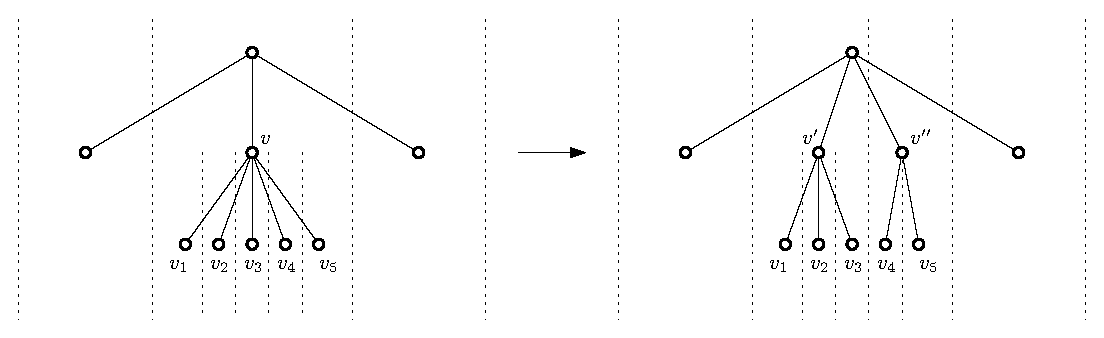
\includegraphics[width=\textwidth]{../figures/arge_split}
     \caption{$v$ is split into $v'$ and $v''$. As a result $Y(v')$ and $Y(v'')$ may contain fewer than $B/2$ points.}
     \label{fig:arge_split_1}
\end{figure}
\begin{figure}[h]
	\centering
	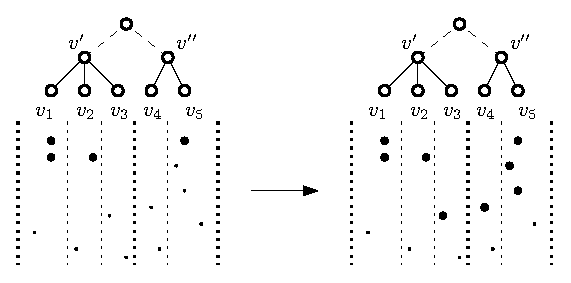
\includegraphics[width=\textwidth]{../figures/arge_split_2}
	\caption{Too small $Y$-sets are remedied by promoting the topmost points from the children.}
	\label{fig:arge_split_2}
\end{figure}


After inserting in the base tree and appropriate reorganization we need to insert the point in the correct query data structure. This is done by starting in the root. The child responsible for the $x$-range which the points belongs to is found and its $Y$-set is found by a degenerate query to the query data structure of the root. If the number of points is $\geq B/2$ and the point is below all of them the point is recursively inserted into the found child. Otherwise the point joins the query data structure of the root. If the $Y$-set of the found child is now too large we recursively insert the lowest of these points into the child's query data structure.
If we reach a leaf we simply insert the point into the query data structure of the leaf.

\subsection{Deletion}
Deleting a point is simple as we adopt global rebuilding to rebalance the tree and not fusion of nodes. To delete a point we search down in the base tree for the point and mark it as deleted without actually removing the point. The next step is to remove the point from the query data structure that it resides in. This is done similar to finding the query data structure to insert the point into. The $Y$-set is recursively found on the search path of the point and if the $Y$-set contains the points, then the point is removed. If the $Y$-set becomes too small as a result we perform a \textit{bubble-up} operation.

\subsection{Analysis}
Inserting in the base tree can be done in $\mathcal{O}(\log_B N)$ I/O's by Section~\ref{sec:prelim_b_tree} and can cause as many splits on the path from a leaf to the root. Each split might cause $B/2$ \textit{bubble-up} operations. Each \textit{bubble-up} at $v$ costs $\mathcal{O}(1)$ I/O's and might recurse all the way to a leaf for a total of $\mathcal{O}(\log_B weight(v))$ where $weight(v)$ is the size of the subtree rooted at $v$. In the worst case $B/2$ of these operations are performed totalling at $\mathcal{O}(B\log_B weight(v)) = \mathcal{O}(weight(v))$ I/O's.

To prove that this gives a cost of $\mathcal{O}(\log_B N)$ I/O's amortized we need the following Lemma from the original paper describing the weight balanced B-tree~\cite{arge_vitter_1996}.
\begin{lemma}
\label{lma:weight_balanced}
After a split of a node $v_l$ on level $l$ into two nodes $v_l'$ and $v_l''$, at least $a^lk/2$ inserts have to pass through $v_l'$ (or $v_l''$) to make it split again. After a new root $r$ in a tree containing $N$ items is created, at least $3N$ inserts have to be done before $r$ splits again.
\end{lemma}

It follows from Lemma~\ref{lma:weight_balanced} that the cost of splitting a node can be amortized over the insertions and thus each of the $\mathcal{O}(\log_B N)$ splits cost $\mathcal{O}(1)$ I/O's amortized.
A proof of Lemma~\ref{lma:weight_balanced} can be found in~\cite{arge_vitter_1996}.

Deleting can be done in $\mathcal{O}(\log_B N)$ I/O's as it is just a search for the point in the base tree and query data structure.

Rebalancing of the tree is done using global rebuilding. After $\Theta(N)$ delete operations the tree is rebuilt using $\mathcal{O}(N \log_B N)$ I/O's which is paid for by double charging the $\Theta(N)$ delete operations.
\section{Query}
\label{sec:arge_query}
Querying the data structure with $Q = \left[ x_1, x_2 \right] \times \left[ y, \infty \right]$ consists of two steps. The first step is to identify which nodes to visit and the second consists of reporting points in $Q$ from the query data structures of the identified nodes. 
We identify which nodes to visit by searching on a path from the root to leaf along paths corresponding to $x_1$ and $x_2$ and visit nodes in between the two paths. As the tree is a search tree on $x$ we know that nodes in between the search paths for $x_1$ and $x_2$ will be in the query range of $Q$.
We will only proceed to visit a child of $v$ if we report all points from the query data structure of $v$ in the $Y$-set of that child with the exception of the leftmost and rightmost paths which are always visited all the way to a leaf.
We do not miss any points, i.e. report all points in $Q$, since, by the rules, a point in $Q$ cannot be in an unvisited subtree as this would have been visited if all points were reported and no points in the subtree has lower $y$-values.

\subsection{Analysis}
In every internal node $v$ visited we spend $\mathcal{O}(1+K_v/B)$ I/O's. There are $\mathcal{O}(\log_B N)$ nodes on the search path from root to the leftmost leaf and rightmost leaf and thus the number of I/O's used on these paths is $\mathcal{O}(\log_B N + K/B)$. All other internal nodes visited are visited because all points were reported in the parent. If we do not report all points from a $Y$-set we can charge the $\mathcal{O}(1)$ I/O's of visiting the child to the parent which must have reported $\Theta(B)$ points. As the cost of reporting from the query data structures is $\mathcal{O}(1+K/B)$ the total cost amounts to $\mathcal{O}(\log_B N + K/B)$.

\chapter{External Memory Buffered Priority Search Tree}
\label{chp:epst}
In this chapter we present an external memory data structure described by Brodal~\cite{DBLP:journals/corr/Brodal15}. The structure supports updates in amortized $\mathcal{O}\left(\frac{1}{\epsilon B^{1-\epsilon}} \log_B N\right)$, three sided range queries in $\mathcal{O}\left(\frac{1}{\epsilon}\log_B N + \nicefrac{K}{B}\right)$ for $0 \leq \epsilon \leq \frac{1}{2}$, and can be constructed on $N$ points in the sorting bound. $\epsilon$ is a parameter that determines the size of the fanout and in turn the size of a bootstrapped substructure for storing $\mathcal{O}(B^{1+\epsilon})$ points, $0 \leq \epsilon \leq \frac{1}{2}$.
The substructure is very similar to that of Arge et al.~\cite[Section~3.1]{arge_vitter_2003} for handling $\Theta(B^2)$ points with the main difference being that we reduce the capacity to allow an amortized constant number of I/O's per update. The bootstrapped structure is in~\cite{arge_vitter_2003} used to store the top $\Theta(B^2)$ points w.r.t. the $y$ value for the subtree rooted at the given node of the substructure. This structure uses it in a slightly different way to store the top $\mathcal{O}(B^{1+\epsilon})$ points of the children of the given  node. This bootstrapped structure is described further in Section~\ref{sec:child_structure} and in the following it will be refered to as the child structure.

The external memory buffered priority search tree is a combination of the external memory priority search tree of Arge et al. described in Chapter~\ref{chp:arge_pst}, and the buffered updates of the buffer tree also thanks to Arge~\cite{Arge:1995:BTN:645930.672850}. The data structure is described in Section~\ref{sec:main_data_structure}.

\begin{figure}
	\centering
	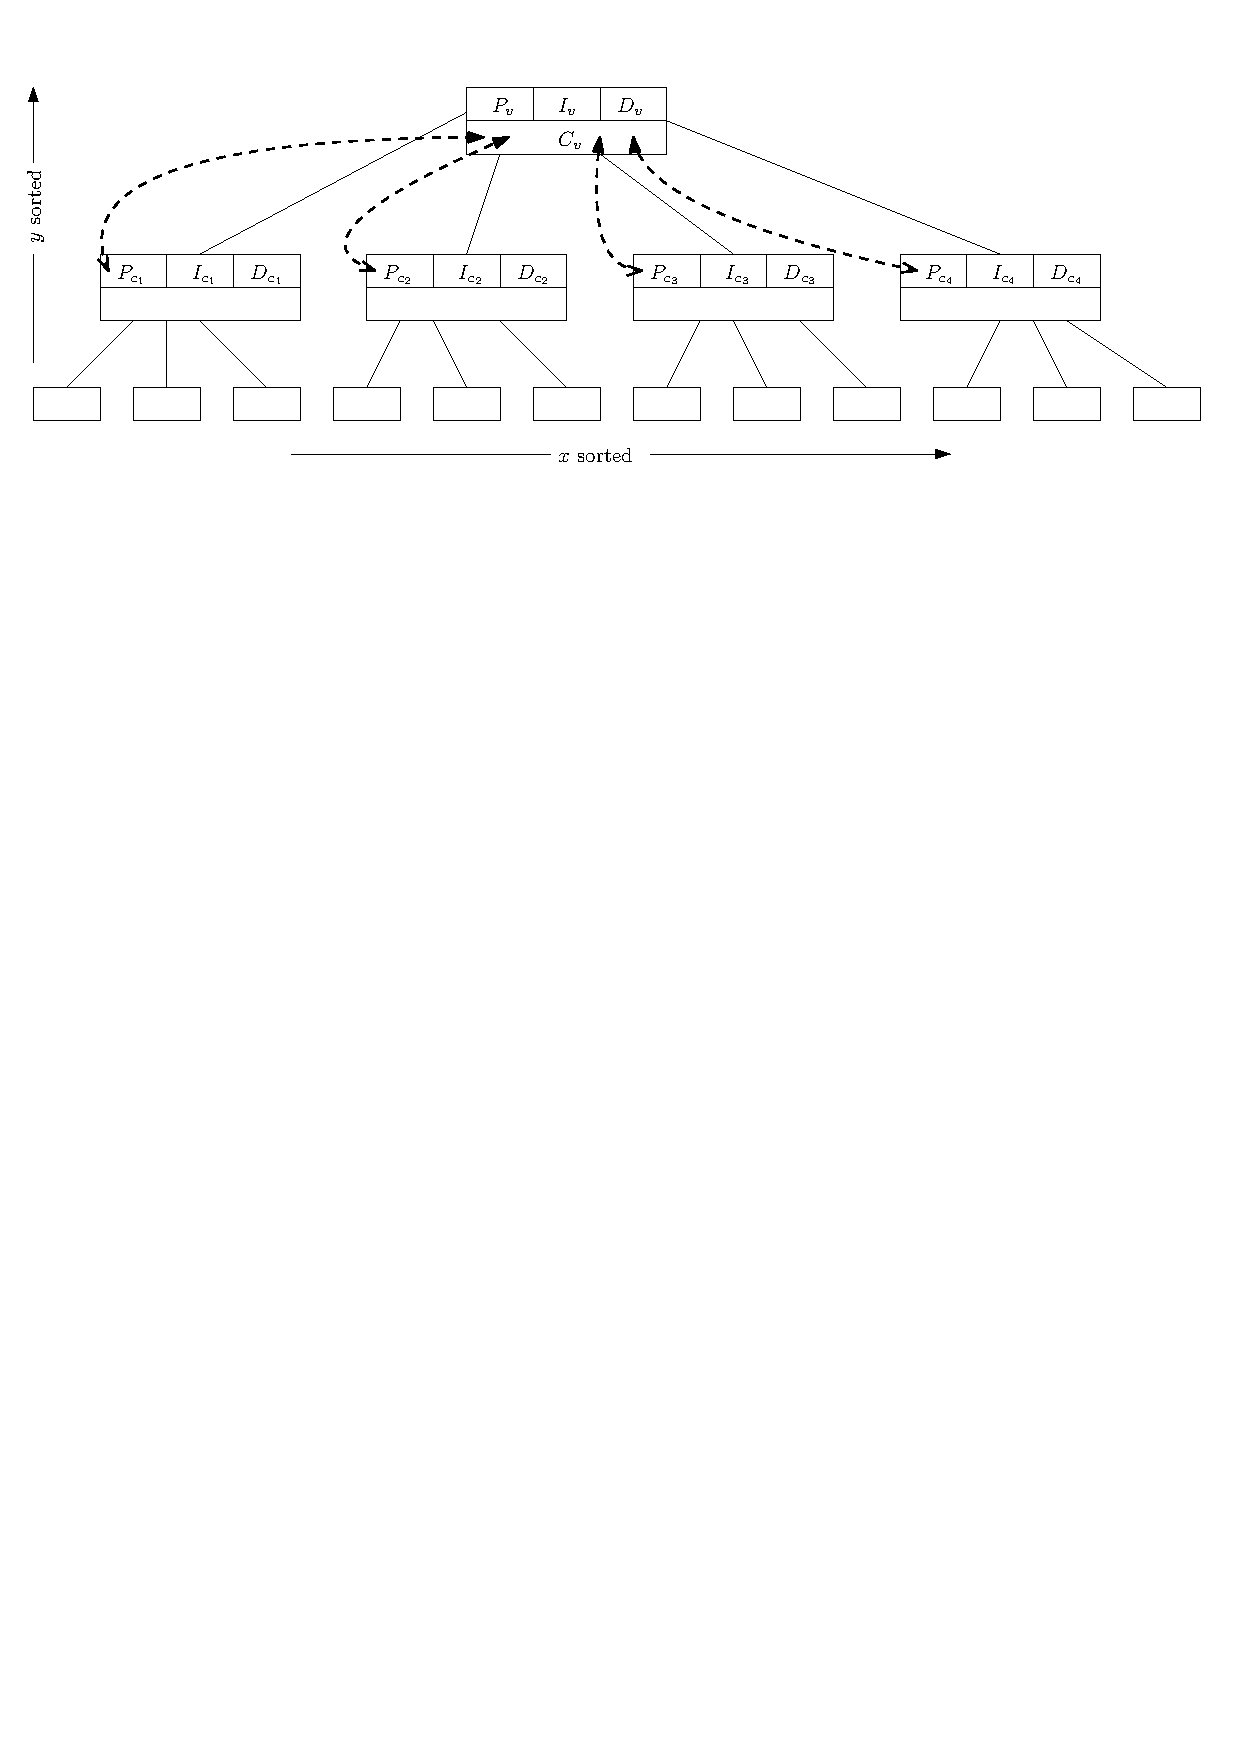
\includegraphics[width=\textwidth]{../figures/gerth_tree}
	\caption{External memory priority search tree with buffers. The point buffers of the children is in the child structure of the parent allowing for fast queries.}
	\label{fig:gerth_tree}
\end{figure}



%%%%%%%%%%%%%%%%%%%%%%%%%
% Main data structure %%%
%%%%%%%%%%%%%%%%%%%%%%%%%

\section{Main data structure}
\label{sec:main_data_structure}
This section presents the main data structure achieving the results of Theorem~\ref{thm:main_structure}.
\begin{theorem}
\label{thm:main_structure}
An external memory data structure exists supporting insertion and deletion of points in amortized $\mathcal{O}(\frac{1}{\epsilon B^{1-\epsilon}} \log_B N)$ I/O's and three sided range queries in amortized $\mathcal{O}(\frac{1}{\epsilon} \log_B N + \nicefrac{K}{B})$, where $\epsilon$ is a constant, $0 < \epsilon \leq \nicefrac{1}{2}$, $N$ is the number of points in the structure, and $K$ is the size of the output. The structure can be constructed in amortized $\mathcal{O}(\nicefrac{N}{B})$ I/O's on an x-sorted set of points and stored in $\mathcal{O}(\nicefrac{N}{B})$ blocks.
\end{theorem}
\todo{Kasper: Skal $\epsilon$ vaere en konstant. I saafald kan man vel bare slette $\frac{1}{\epsilon}$ ledet?}

The structure is a slightly modified version of the B-tree. Each internal node, except for the root, has a degree between $\frac{\Delta}{2}$ and $\Delta$, with $\Delta = \lceil B^\epsilon \rceil$. The root has degree between $2$ and $\Delta$.

Each node $v$ stores three buffers containing $\mathcal{O}(B)$ points each. A point buffer $P_v$, an insertion buffer $I_v$, and a deletion buffer $D_v$.

The subtree at node $v$ contains points in the range spanned by the points in the point buffer $P_v$, i.e. the structure is a search tree on the points in $P_v$ w.r.t. to the normal lexicographical ordering of points.

As in the internal priority search tree the points with highest $y$-value resides in the top of the tree, i.e. we have a heap ordering among the nodes of the tree on the $y$-value. This means that for a node $v$, no child $c$ of $v$ stores an element in $P_c$ with a larger $y$-value than the minimum $y$-value in $P_v$.
$I_v$ and $D_v$ stores buffered insertions and deletions on their way down to a point buffer of a descendent and are handled recursively whenever a buffer overflows.

For each internal node, $v$, we also store an instance of the child structure, $C_v$, containing the elements $P_c$ for every child $c$ of $v$.

Finally, for each internal node, $v$, we store, in $\mathcal{O}(1)$ blocks, information about the minimum $y$-value of the points of each of $v$'s children or $\infty$ if the child does not store any points.

All information at the root is kept in internal memory except for the child structure.
\todo{Kasper: Hvorfor ikke child structure?}

\subsection{Invariants}
For a node $v$ in the main data structure the following invariants must be true:
\begin{itemize}
	\item $P_v$, $I_v$, and $D_v$ are disjoint and points in the buffers have $x$-values spanned by the subtree at $v$.
	\item All points in $I_v \cup D_v$ have $y$-value less than the points in $P_v$.
	\item An update in a buffer at $v$ is more recent and should eventually overwrite any update in a descendent of $v$ with the same point.
	\item A leaf in the tree has empty insertion and deletion buffers and the size of its point buffer is less than $B/2$.
	\item An internal node in the tree has $B/2 \leq \vert P_v \vert \leq B$, $\vert D_v \vert \leq B/4$, and $\vert I_v \vert \leq B$.
\end{itemize}

\subsection{Updates}
\label{subsec:gerth_updates}
We update the structure by adding points to either the insertion or deletion buffer of the root while maintaining the above invariants.
To be able to maintain the above invariants we must be very careful whenever we update the data structure. During an update the insertion or deletion buffers might overflow. This is handled in the following five steps:
\begin{inlinelist}
	\item handle overflowing deletion buffers
	\item handle overflowing insertion buffers
	\item split leaves with overflowing point buffers
	\item split nodes of degree $\Delta+1$
	\item fill underflowing point buffers
\end{inlinelist}

We will in the following look at each step individually and argue their complexity.

\begin{enumerate}[label=(\roman*)]
	\item\label{update:del} A deletion buffer at node $v$ overflows when $\vert D_v \vert > B/4$. Since the structure is a B-tree on the lexicographically ordering of points we must by the pigeon-hole principle have that there exist a child $c$ such that we can push $U \subseteq D_v$ of $\lceil \vert D_v \vert / \Delta \rceil$ deletions to $c$. This is illustrated in Figure~\ref{fig:pigeon_hole}. Points in $U$ are removed from $D_v$, $I_c$, $D_c$, $P_c$, and $C_v$. Any point $p$ in $U$ lexicographically larger than the minimum point in $P_c$ (w.r.t. $y$) is removed from $U$ as the deletion cannot cancel any updates further down in the tree.
	
	\begin{figure}[htp!]
		\centering
		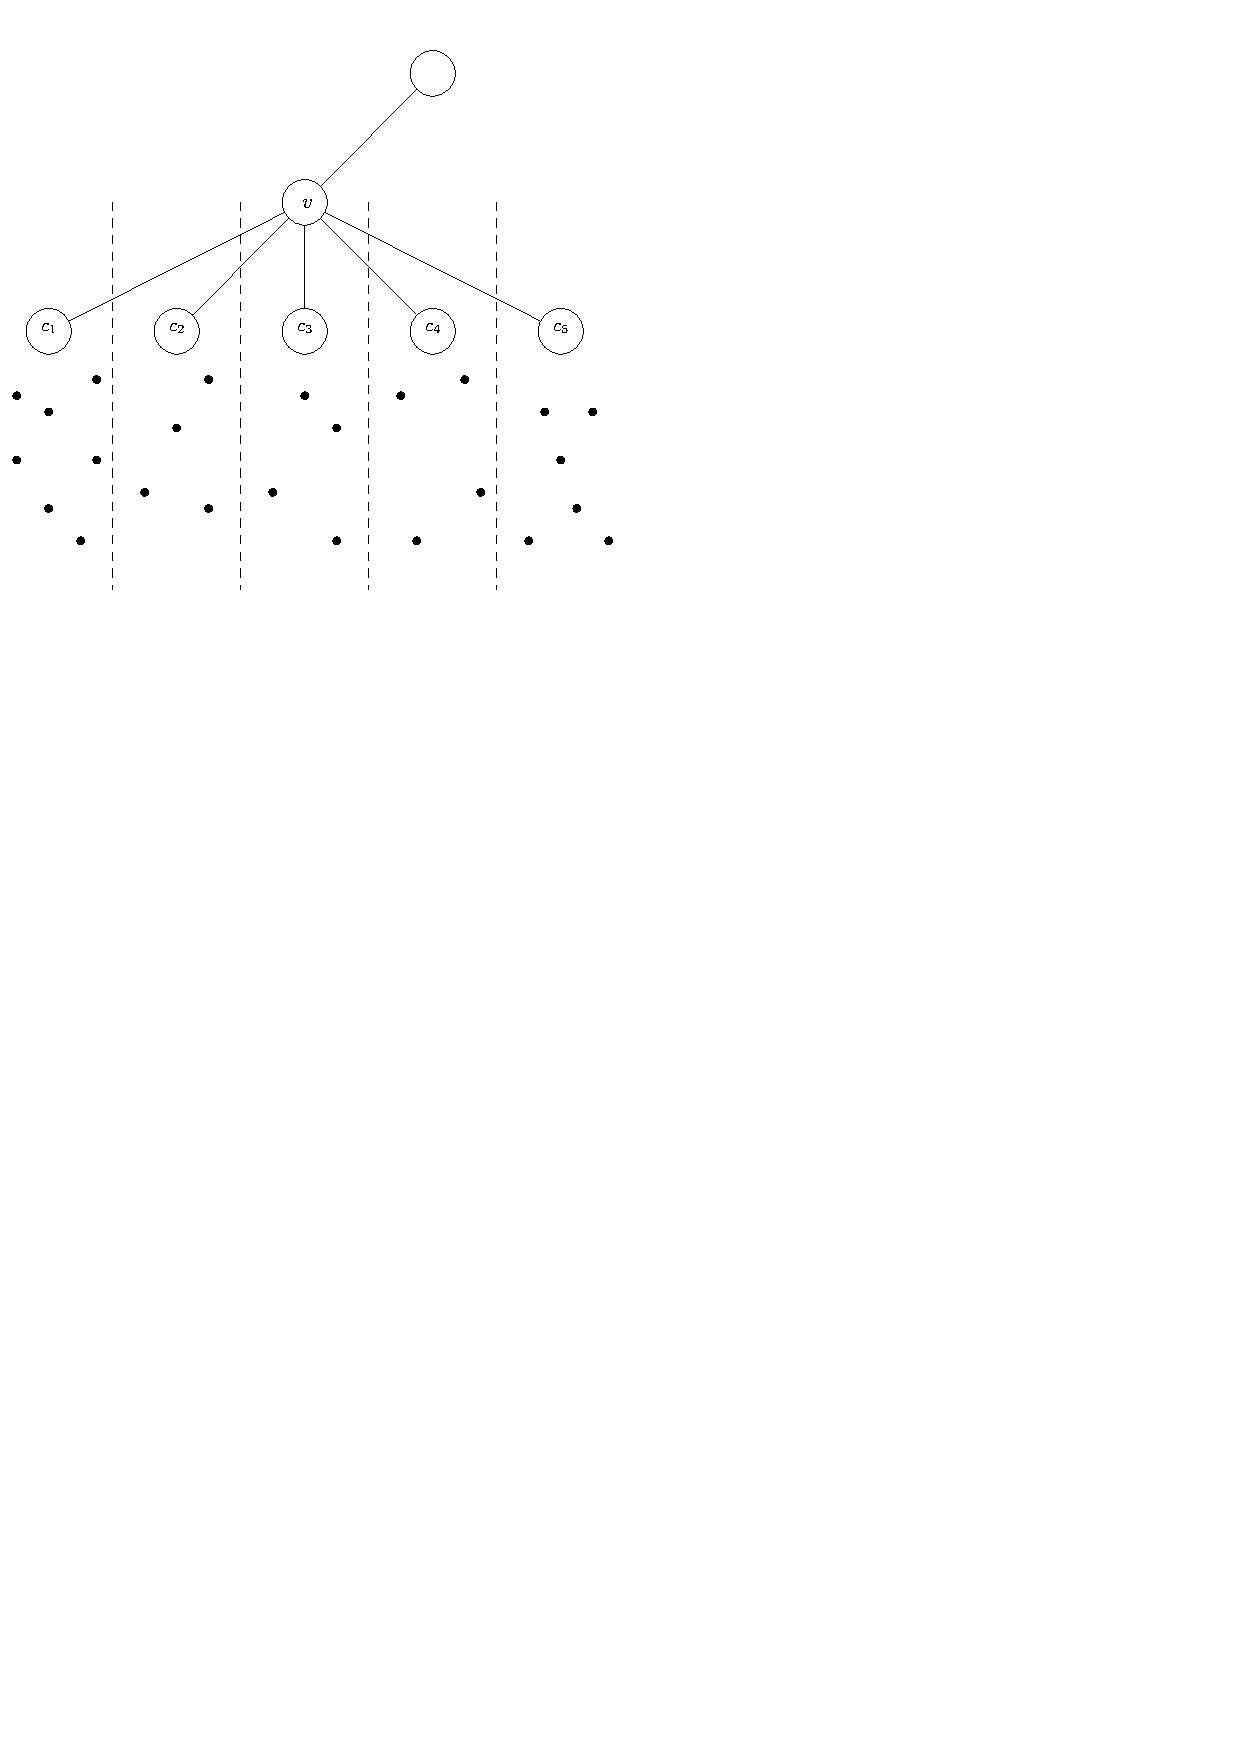
\includegraphics[width=\textwidth]{../figures/pigeon_hole}
		\caption{Each point represents a deletion. $B=25$ and $\epsilon = 0.5$. This gives $B^{\epsilon} = 5$. By the pigeon hole principle we must have that at least one of the x-ranges contains $\frac{B}{B^\epsilon}$ points.}
		\label{fig:pigeon_hole}
	\end{figure}
	
	If $v$ is a leaf we do not need to do more. If not, the remaining points in $U$ are inserted in $D_c$ which might recursively overflow. In the worst case we might recursively overflow along a path from the root to a leaf each time causing $\mathcal{O}(\lceil \vert B \vert / \Delta \rceil)$ deletes to be pushed one level down. Updating $C_v$ with $\mathcal{O}(\lceil \vert B \vert / \Delta \rceil)$ updates takes amortized $\mathcal{O}(1+ (B/\Delta) / B^{1-\epsilon}) = \mathcal{O}(1)$ I/O's.
	
	\item\label{update:ins} An insertion buffer at $v$ overflows when $\vert I_v \vert > B$. Similar to handling a deletion buffer overflow we find a child $c$ such that we can push $U \subseteq I_v$ of $\lceil \vert D_v \vert / \Delta \rceil$ insertions to $c$. Points in $U$ are removed from $I_v$, $I_c$, $D_c$, $P_c$, and $C_v$.
	Any point $p$ in $U$ lexicographically larger than the minimum point in $P_c$ (w.r.t. $y$) is removed from $U$ and inserted into $P_c$ and $C_v$.
	If $P_c$ overflows, the lexicographically smallest points w.r.t. $y$ are moved from $P_c$ to $U$ until $P_c$ no longer overflows.
	If $c$ is a leaf then all points are inserted into $P_c$ and $U$ is now empty.
	Otherwise, the remaining points in $U$ are added to $I_c$ which might overflow and cause a similar overflow along a path from the root to a leaf in the worst case as in the case of the deletion buffer overflow.
	
	\item\label{update:pbo} A point buffer overflows at a leaf $v$ when $\vert P_v \vert > B/2$. If this is the case then we split the leaf into two nodes and evenly distribute the points in $P_v$ among the two new nodes using $\mathcal{O}(1)$ I/O's. The splitting of the node might cause the parent to get a degree of $\Delta+1$.
	
	\item\label{update:deg} An internal node $v$ with a degree larger than $\Delta$ is split into two new nodes $v'$ and $v''$. $I_v$, $D_v$, and $P_v$ are distributed among $v'$ and $v''$ according to the $x$-value. Finally the child structures of $v'$ and $v''$ are rebuilt from the children's point buffers. The split might cause the parent of $v$ to have a degree overflow and in the worst case we need to split along a path from a leaf to the root. The splitting of a single node costs $\mathcal{O}(\Delta)$ I/O's due to the reconstruction of the child structures.
	
	\item\label{update:pbu} A point buffer underflows at $v$ when $\vert P_v \vert < B/2$. In that case we try to move the highest $B/2$ points from the children of $v$ into $P_v$. If $v$'s subtree does not store any points then we remove all points from $D_v$ and move points from $I_v$ to $P_v$ until $\vert P_v \vert = B$ or $I_v = \emptyset$.
	Otherwise we use $\mathcal{O}(\Delta)$ I/O's to identify $X$ as the top $B/2$ points from the children of $v$ and remove the identified points from the point buffers of the children and the child structure of $v$.

	If a point buffer of a child becomes empty before having identified all of the top $B/2$ points we have to recursively fill that child as the subtree might contain points with larger $y$-value than the remaining children of $v$. After this is done we can continue to grab points from the children.
	
	All points in $X \cap D_v$ are removed from $X$. This might cause the point buffer of $v$ to become empty once again and the procedure must be repeated.
	
	The remaining points of $X$ are inserted into $P_v$ and the child structure of the parent of $v$.	
	
	The points of $X$ now inserted into $P_v$ might have a smaller $y$ value than the points in $I_v$. We solve this problem by swapping the highest point in $I_v$ with the lowest point in $P_v$ while there exists a point in $I_v$ that is higher than a point in $P_v$.	
	
	If the subtree of $v$ becomes empty as a result of pulling points up to $v$ we must remove all points of $D_v$ and move points from $I_v$ to $P_v$. This might cause $P_v$ to overflow.
	
	Finally, after having pulled points from the children, we check if any of the children's point buffers underflows and should be refilled.
\end{enumerate}

\textbf{Analysis}

The tree grows in height during insertions by splitting leaves and internal nodes which also keeps the tree balanced. We stay balanced during insertions since we only increase in height whenever the root splits which causes every path from root to leaf to increase by one. In the B-tree we handle rebalancing using fusion of nodes. We do not apply this method here but instead apply global rebuilding when a linear number of updates have been performed. By~\ref{update:pbo} it follows that the total number of leaves created during $N$ insertions can be at most $\mathcal{O}(N/B)$ implying that at most $\mathcal{O}(\frac{N}{\Delta B})$ internal nodes can be created by splitting internal nodes. From this it follows that the tree has height $\mathcal{O}(\log_\Delta \frac{N}{B}) = \mathcal{O}(\frac{1}{\epsilon} \log_B N)$.

We can now argue that every update in~\ref{update:del} and~\ref{update:ins} requires amortized $\mathcal{O}(\frac{1}{\epsilon B^{1-\epsilon}} \log_B N)$ I/O's. As every $\Theta (B/\Delta)$ update require $\mathcal{O}(1)$ I/O's on every layer of the tree we get the correct amortized bound:
\begin{align*}
\mathcal{O}(\frac{1}{B/\Delta} \log_\Delta \frac{N}{B}) &= \frac{B^\epsilon}{B} \log_{B^\epsilon} \frac{N}{B} \\
&= \frac{B^\epsilon}{B} \frac{1}{\epsilon} \log_{B} N \\
&= \frac{1}{\epsilon B^{1-\epsilon}} \log_B N
\end{align*}

In~\ref{update:pbo}, we know that at most $\mathcal{O}(N/B)$ leaves are created each requiring $\mathcal{O}(1)$ I/O's giving amortized $\mathcal{O}(1/B)$ I/O's per update.

In~\ref{update:deg}, we know that at most $\mathcal{O}(\frac{N}{B\Delta})$ internal nodes are created. The creation of such a node costs $\mathcal{O}(\Delta)$ giving an amortized cost of $\mathcal{O}(1/B)$ I/O's per update.

In~\ref{update:pbu} each refilling might trigger a cascaded recursive refilling of one or more of the children. Every refilling takes $\mathcal{O}(\Delta)$ I/O's and moves $\Theta(B)$ points one level up through the tree's point buffers. Each point can at most move $\mathcal{O}(\log_\Delta \frac{N}{B})$ levels up, as this is the tree's height. This means that the total number of I/O's for the refillings during the course of $N$ operations is amortized $\mathcal{O}(\frac{1}{B/\Delta} \log_\Delta \frac{N}{B}) = \frac{1}{\epsilon B^{1-\epsilon}} \log_B N$ per point.

This argument ignores the fact that when pulling up points some points might swap positions from $I_v$ to $P_v$. This swap does not change the fact that the number of points we pull up remain the same and therefore it does not change the amortized accounting.

Another fact that we ignore is what happens if we are not able to pull up $B/2$ points from the children. This is solved by a simple amortization argument. We double charge the operation responsible for pushing points to a child. This way we can ensure each node with non-empty point buffers always has saved an I/O for being emptied by a recursive pull up.

\subsection{Global rebuilding}
As we do not fuse nodes with too low node degree we might end up with an unbalanced tree. We use global rebuilding as described in Section~\ref{sec:prelim_global_rebuilding} to guarantee that the tree is rebalanced and thus that our amortized bounds hold.
Updates are partitioned into epochs. After a rebuild a new epoch begins and if the data structure at this points stores $\bar{N}$ points, then the next epoch will begin after $\bar{N}/2$ updates, i.e. a global rebuild will be performed.
Having a new epoch after every $\bar{N}/2$ updates ensures that our tree does not grow higher than $\mathcal{O}\left(\frac{1}{\epsilon}\log_B\frac{3\bar{N}}{2}\right) = \mathcal{O}\left(\frac{1}{\epsilon}\log_B N\right)$ as the size is $\frac{1}{2}\bar{N} \leq N \leq \frac{3}{2}\bar{N}$.

Global rebuilding works by constructing an empty structure and then reinserting all the points of the old structure that has not been deleted.

The points to reinsert are found by doing a top-down traversal of the tree while flushing insertion and deletion buffers to children. The points to reinsert are then found in the point buffers after flushing. This might cause buffers to temporarily overflow but we will allow this as the old structure will be deleted.

Once the set of points to reinsert have been found we simply insert the points on an initially empty tree.

\textbf{Analysis}

Elements at level $i$ (leaf layer being level 0) can at most be flushed $i$ levels down.
The structure holds at most $\frac{3\bar{N}}{2B}$ nodes in total and at level $i$ the structure has at most $\frac{3\bar{N}}{2B} \frac{1}{\Delta^i}$ nodes. The cost of flushing all the buffers at level $i$ becomes:

$$ i \cdot \frac{3\bar{N}}{2B} \frac{1}{\Delta^i}$$

By summing over all layers of the tree we get the total cost of flushing all buffers to be:
\begin{align*}
\sum\limits_{i=0}^{\mathcal{O}(\log_\Delta \frac{3N}{2B})} i \cdot \frac{3\bar{N}}{2B} \frac{1}{\Delta^i} &< 
\sum\limits_{i=0}^{\infty} i \cdot \frac{3\bar{N}}{2B} \frac{1}{\Delta^i} \\
&= \frac{3\bar{N}}{2B} \sum\limits_{i=0}^{\infty} \frac{i}{\Delta^i} \\
&= \frac{3\bar{N}}{2B} \sum\limits_{i=0}^{\infty} \left(\frac{1}{\Delta}\right)^i \\
&= \frac{3\bar{N}}{2B} \frac{1}{1-\Delta} \\
&= \mathcal{O}(N/B)
\end{align*}

This gives an amortized cost of $\mathcal{O}(1/B)$ per update to flush all buffers.

The $\mathcal{O}(\bar{N})$ reinsertions into the new tree can be done in amortized $\mathcal{O}(\nicefrac{\bar{N}}{\epsilon B^{1-\epsilon}} \log_B N)$ I/O's are paid by the $\bar{N}/2$ updates during the epoch.

%\includegraphics[width=\textwidth]{../handwritten notes/Notes on global rebuilding analysis.jpg}

\subsection{Three sided range queries}
\label{subsec:brodal_3_sided}
Reporting a query $Q = \left[ x_1,x_2 \right] \times \left[y, \infty \right]$ consists of three steps. Identifying the nodes to visit, push down delayed insertions and deletions between these identified nodes, and finally reporting the points in $Q$.

We identify the nodes to visit in a breadth first manner.
Starting from the root we identify, from the query's $x$-range, the children that are relevant to the query and push all insertions and deletions in the root to the identified children without handling possible overflows. After having done this we know that the point buffers of the children do not change further and we can thus report all points in the query range from the child structure of the root and the point buffer of the root. The children worth visiting are added to the back of the breadth first search queue. We can decide whether a child is worth visiting without reading the node by comparing $y$ with the minimum $y$-value of that child's point buffer. This value is stored in the parent.
All nodes other than the root do not need to report from their point buffers as the parent of the node has already reported the relevant points from the child structure.

After all points have been reported we might have some buffers that have temporarily overflowed. This is now handled in a bottom up fashion using the update operations described in Subsection~\ref{subsec:gerth_updates}. We will handle a single subtree at a time and make sure that the entire subtree has no buffers that overflow or underflow or any nodes with a too high node degree. We do this by the update operations~\ref{update:del}-\ref{update:deg} and at the same time we disallow that any recursion leaves the subtree, i.e. no splits may recursively split nodes outside of the subtree. When the entire subtree has no overflows or underflows we can remedy a potential underflowed point buffer using update operation~\ref{update:pbu} and continue to the next subtree one level higher in the tree.

This process could also be described recursively. The base case of the recursion is the leaf $l$ which is handled by moving points from $I_l$ into $P_l$ and potentially splitting. At a layer above $l$ at node $v$ we might have many children which are all leafs and handled according to the base case. Node $v$ is now handled as described before and we have thus taken a step in the recursion. This process continues up to the root of the tree leaving the tree in a state with no overflows or underflows.

\begin{figure}
\centering
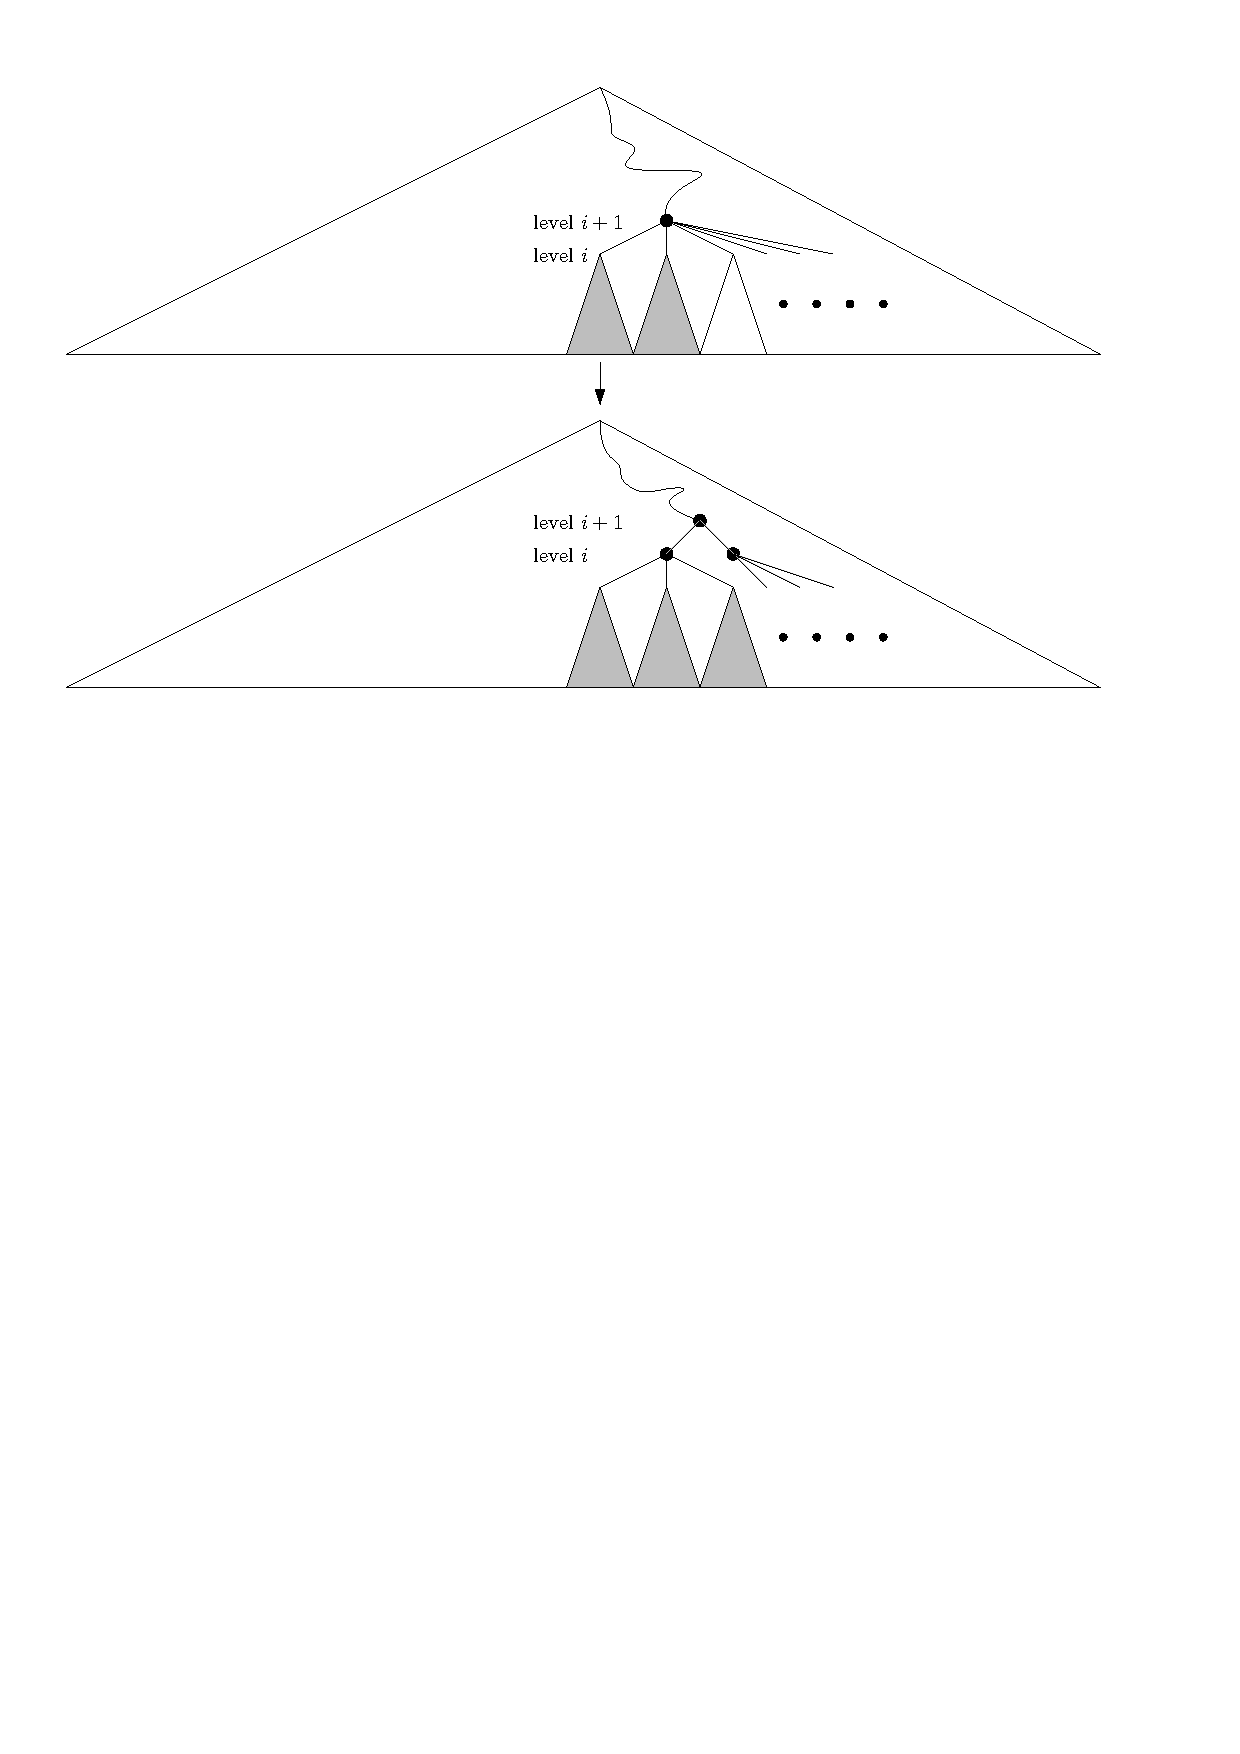
\includegraphics[width=\textwidth]{../figures/gerth_fixup}
\caption{missing}
\label{fig:gerth_fixup}
\end{figure}

\textbf{Analysis}

Assume that during a query we visit $V$ nodes that are not on the search paths for $x_1$ or $x_2$ and $\mathcal{O}(\frac{1}{\epsilon}\log_B N)$ nodes on the search paths. We know that the $V$ nodes must have atleast $VB/2$ points in their point buffers before pushing down updates. The number of deletions we push down to visited nodes can at most be $(V + \mathcal{O}(\frac{1}{\epsilon}\log_B N))B/4$. It now follows that the number of points that we report, $K$, must be atleast the number of points in the point buffers before pushing down minus the deletions that we push down: $VB/2 - (V + \mathcal{O}(\frac{1}{\epsilon}\log_B N))B/4 = VB/4 - \mathcal{O}(\frac{B}{\epsilon}\log_B N) = K$. By isolating $V$ it follows that $V = \mathcal{O}(\frac{1}{\epsilon}\log_B N + K/B)$.

The worst case bound now becomes the sum of visiting the $V$ nodes, the nodes on the search paths for $x_1$ and $x_2$, and the output: $\mathcal{O}(V+\frac{1}{\epsilon}\log_B N + K/B) = \mathcal{O}(\frac{1}{\epsilon}\log_B N + K/B)$.
On top of this comes the cost of pushing down update buffer elements and handling overflowing update buffers and overflowing point buffers.

This cost of pushing $\Omega(B/\Delta)$ is however already paid for by the update operations and is thus covered by the analysis of Subsection~\ref{subsec:gerth_updates}. It is only when we push down $\mathcal{O}(B/\Delta)$ updates to a child, with an amortized cost of $\mathcal{O}(1)$, that this cost is covered by the cost of visiting the child.

Handling the overflowing update buffers and underflowing point buffers is also paid by the update operations and thus the analysis in Subsection~\ref{subsec:gerth_updates}.

It all adds up to a total amortized cost of $\mathcal{O}(\frac{1}{\epsilon} \log_B N + K/B)$ I/O's for a 3-sided range query.

\subsection{Construction}
The structure can be initialized with an initial set of $N$ points using just $\mathcal{O}(\text{Sort}(N))$ I/O's. If the points are already sorted on $x$ we just need $\mathcal{O}(\text{Scan}(N))$. For the remainder of this Section we assume that the points are initially sorted with regards to $x$.

The first step of the construction is to construct a B-tree with each internal node having a degree of $\Delta/2$ over the $x$-values such that each leaf stores $\nicefrac{B}{2}$ points with the exception of the rightmost leaf which might contain less than $\nicefrac{B}{2}$ points and the rightmost internal nodes having a degree less than $\Delta/2$.

The point buffers of the internal nodes are now filled bottom up pulling the top $B/2$ highest $y$-value points up. If this results in a child having an underflowing point buffer we recursively fill that child before proceeding. In a second iteration we do the same but in a top-down fashion.

All insertion and deletion buffers are initially empty and the child structures are constructed from the point buffers of the children.

This construction algorithm could also have been used for global rebuilding giving a matching amortized cost.

\begin{figure}
	\centering
	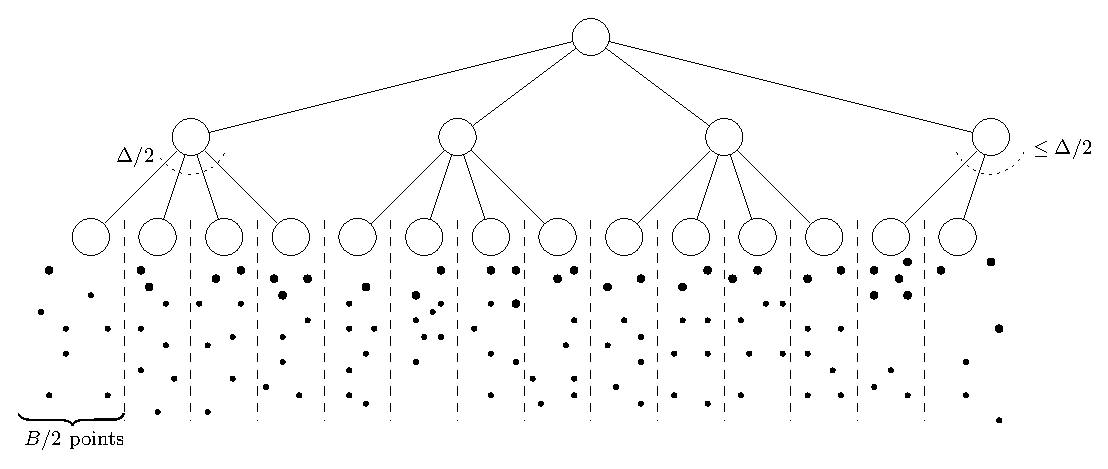
\includegraphics[width=\textwidth]{../figures/gerth_construction}
	\caption{A B-tree with each internal node having a degree of $\Delta/2$. Each leaf stores $B/2$ points with the exception of the rightmost. The marked points are the top $B/2$ points that is pulled up from the leaves into the layer above.}
	\label{fig:gerth_construction}
\end{figure}

\textbf{Analysis}

We have that level $i$ of the tree contains at most $\frac{N}{B\Delta^i}$ nodes. It follows that the number of points stored at or above level $i$ is $\mathcal{O}(\sum\limits_{j=i}^\infty B\frac{N}{B\Delta^j}) = \mathcal{O}(\frac{N}{\Delta^i})$. This must mean that we cannot move $B/2$ points to level $i$ from $i-1$ more than $\mathcal{O}(\frac{N}{\Delta^i} / \frac{B}{2})$ times. We know that we can move $B/2$ points using $\mathcal{O}(\Delta)$ I/O's and the total number of I/O's to fill the point buffers becomes:
$$\mathcal{O}\left(\sum\limits_{i=1}^\infty \Delta \frac{N}{B\Delta^i}\right) = \mathcal{O}\left(\frac{N}{B}\sum\limits_{i=1}^\infty \Delta \frac{1}{\Delta^i}\right) = \mathcal{O}\left(\frac{N}{B}\sum\limits_{i=0}^\infty \frac{1}{\Delta^i}\right) = \mathcal{O}\left(\frac{N}{B}\right)$$

Another aspect we have to look at is what happens to the amortized analysis when we initialize our data structure using this construction method, i.e. we have to argue that the amortized cost of the remain unchanged during the epoch started by the construction.

In order to argue this we consider a sequence of operations containing $N_{ins}$ insertions and $N_{del}$ deletions and a newly constructed tree of $N$ points.

Let us first consider the cost of creating new nodes in the tree. Each leaf has initially at most $B/2$ points and it follows that we can at most create $2N_{ins}/B$ new leaves. Each new leaf is created in $\mathcal{O}(1)$ I/O's and it thus cost at most $\mathcal{O}(N_{ins}/B)$ I/O's to create new leaves during $N_{ins}$ insertions.
By a similar argument it follows that at most $\mathcal{O}(\frac{N_{ins}}{\Delta B})$ new internal nodes can be created since each internal node initially has a degree of $\leq \Delta/2$. Each new internal node is created in $\mathcal{O}(\Delta)$ I/O's and it thus costs $\mathcal{O}(N_{ins}/B)$ I/O's to create new internal nodes without the cost of refilling point buffers which we look at below.

An insertion has to be moved at most the height of the tree levels down before it is cancelled or moved into a point buffer. Since the height of the tree is $\mathcal{O}(\frac{1}{\epsilon} \log_B N)$ it follows that the cost of handling overflowing insertions buffers during the course of $N_{ins}$ insertions becomes $\mathcal{O}(\frac{N_{ins}}{B/\Delta}\frac{1}{\epsilon}\log_B N)$ I/O's.
A similar argument can be given for the case of deletions.

Each deletion leaves behind a hole which needs to be filled. This hole is filled by recursively pulling up points which effectively moves down the hole. Each split of internal nodes also potentially creates up to $B$ holes.
In total we need to handle $\mathcal{O}(N_{del} + \frac{N_{ins}}{\Delta B})$ holes. We can move up $B/2$ points using $\mathcal{O}(\Delta)$ I/O's and they at most need to be moved to the top of the tree, i.e. they need to be at most moved the height of the tree levels up. This gives a total cost of $\mathcal{O}((N_{del} + \frac{N_{ins}}{\Delta B})\frac{\Delta}{B}\frac{1}{\epsilon} \log_B N)$ I/O's.

All this adds up to $\mathcal{O}(\frac{N_{ins}+N_{del}}{B/\Delta} \frac{1}{\epsilon} \log_B N) = \mathcal{O}(\frac{N_{ins}+N_{del}}{\epsilon B^{1-\epsilon}} \log_B N)$  I/O's for handling updates. This matches the amortized bounds of the structure.
\todo{Figures}

\chapter{Other structures}

\section{R-tree}

\todo{$\log_B N$ I/Os for updates. N/B + K I/Os for query.}

\todo{While much work has been done on evaluating the practical
query performance of the R-tree variants mentioned
above, very little is known about their theoretical worst-case
performance. Most theoretical work on R-trees is concerned
with estimating the expected cost of queries under assumptions
such as uniform distribution of the input and/or the
queries, or assuming that the input are points rather than
rectangles.}

The R-tree was introduced by Antonin Guttman in~\cite{Guttman:1984:RDI:602259.602266}. The structure is heuristic in nature and does not provide any close to optimal search bounds. Arge et al. has, however, provided strong evidence for R-trees outperforming several theoretical optimal data structures in practice in~\cite{Arge:2008:PRP:1328911.1328920}. We will introduce the important ideas of the R-tree.

Let $P$ be a set of points. An R-tree stores all points from $P$ in leaf nodes, each of which contains $\Theta(B)$ points. Each non-leaf node $u$ has $\Theta(B)$ children, except for the root which must have 2 children unless it is the only node in the tree. For each child $v$, $u$ stores a \textit{minimum bounding rectangle} (MBR), which is the smallest rectangle that \textit{tightly} encloses all the data points in the subtree of $v$. Note that there is no constraint on how points should be grouped into leafs nodes. Also, there is no constraint on how non-leaf nodes should be grouped in higher level nodes. Since each point is stored only once, the entire data structure consumes linear space. Please refer to figure~\ref{fig:r_tree_structure} for an illustration of an R-tree structure.

\begin{figure}[h]
	\centering
     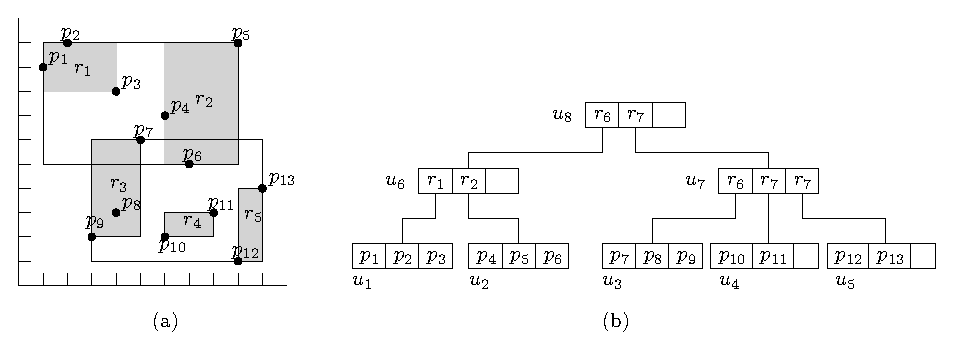
\includegraphics[width=\textwidth]{../figures/r_tree_data_and_mbrs}
     \caption{(a) Data and MBRs (b) The R-Tree structure}
     \label{fig:r_tree_structure}
\end{figure}

\subsection{Query}
Given a query rectangle $q$ we want to find all the points in $P$ that are covered by $q$. The relation to the R-tree is that we only need to visit those nodes whose MBRs intersect $q$. Intuitively, this means that we desire as \textit{small} MBRs as possible, as this directly implies that we a query ispans fewer MBRs leading to fewer nodes to be visited. A good heuristic is therefore to minimize the perimeter of each MBR as this directly implies MBRs that covers smaller areas.

\subsection{Insertions}
To insert a point $p$, we add $p$ to a lead node $u$ by following a single root-to-leaf path. If $u$ overflows we split it, which create a new child of $parent(u)$. This could cause $parent(u)$ to overflow which is handled in a recursive manner. Finally, if the root split, then a new root is created. Note that is legal to insert a point $p$ into \textit{any} leaf after which the data structure will still be considered legal. This is the main property that differs R-trees from standard B-trees. There are several different heuristics for chosing a subtree to insert that all gives rise to different R-tree names. We will cover the original R-tree heuristic and the R$^*$-tree.

The formal definition of inserting a new point $p$ is as follows. Given a non-leaf $u$ with children $v_1, v_2, \cdots, v_{\Theta(B)}$, we need to pick the best child $v^*$ such that the new point $p$ is best inserted into the subtree of $v^*$.

\textbf{Choosing a subtree to insert in an R-tree.}  The standard R-tree chooses the best child in a greedy manner. Specifically, $v^*$ is simply the child $v_i$ whose MBR requires the \textit{least increase} of area in order to cover $p$.

\textbf{Choosing a subtree to insert in an R$^*$-tree.} The problems in the original R-Tree is that certain types of data may create small areas but large distances which will initiate a bad split. To overcome this, a mixed heuristic is employed. At leaf level we try to minimize the overlap and in case of \textit{ties} the MBR that requires the \textit{least increase} of perimeter is chosen. If this again yields a tie the MBR that increases the least in area is chosen. At the higher levels, it behaves similar to the R-tree.

\textbf{Node split in an R-Tree} was originally proposed done by Guttman using two different heuristics. The \textit{linear method} chooses far apart nodes as ends. Randomly nodes are then chosen and assigned such that require the smallest MBR enlargment. The \textit{quadratic method} chooses two nodes so the dead space between them is maximized. Nodes are then assigned such that MBR area is minimized.

\textbf{Node split in an R$^*$-Tree is fairly more involved} but the main idea is to always split point set $S$ using an axis-orthogonal cut. This means that points of $S$ is sorted with respect to their $x$- and $y$-value respectively. Then, the first $\nicefrac{B}{2}$ points are inserted into $S_1$ and the rest is inserted into $S_2$ for the $x$-sorted points and into $S'_1$ and $S'_2$ for the $y$-sorted points. The final split is the better one of the two splits, i.e. the splits that have the least combined MBR perimeter and least combined MBR area. The above applies to splitting of a leaf node. The case of a non-leaf node is a bit different because the items be split are MBRs. The strategy is however the same and involves sorting the MBRs by their centroids. Please refer to figure~\ref{fig:r_tree_splitting} for an illustration of the splitting of a node.

\begin{figure}[h]
	\centering
     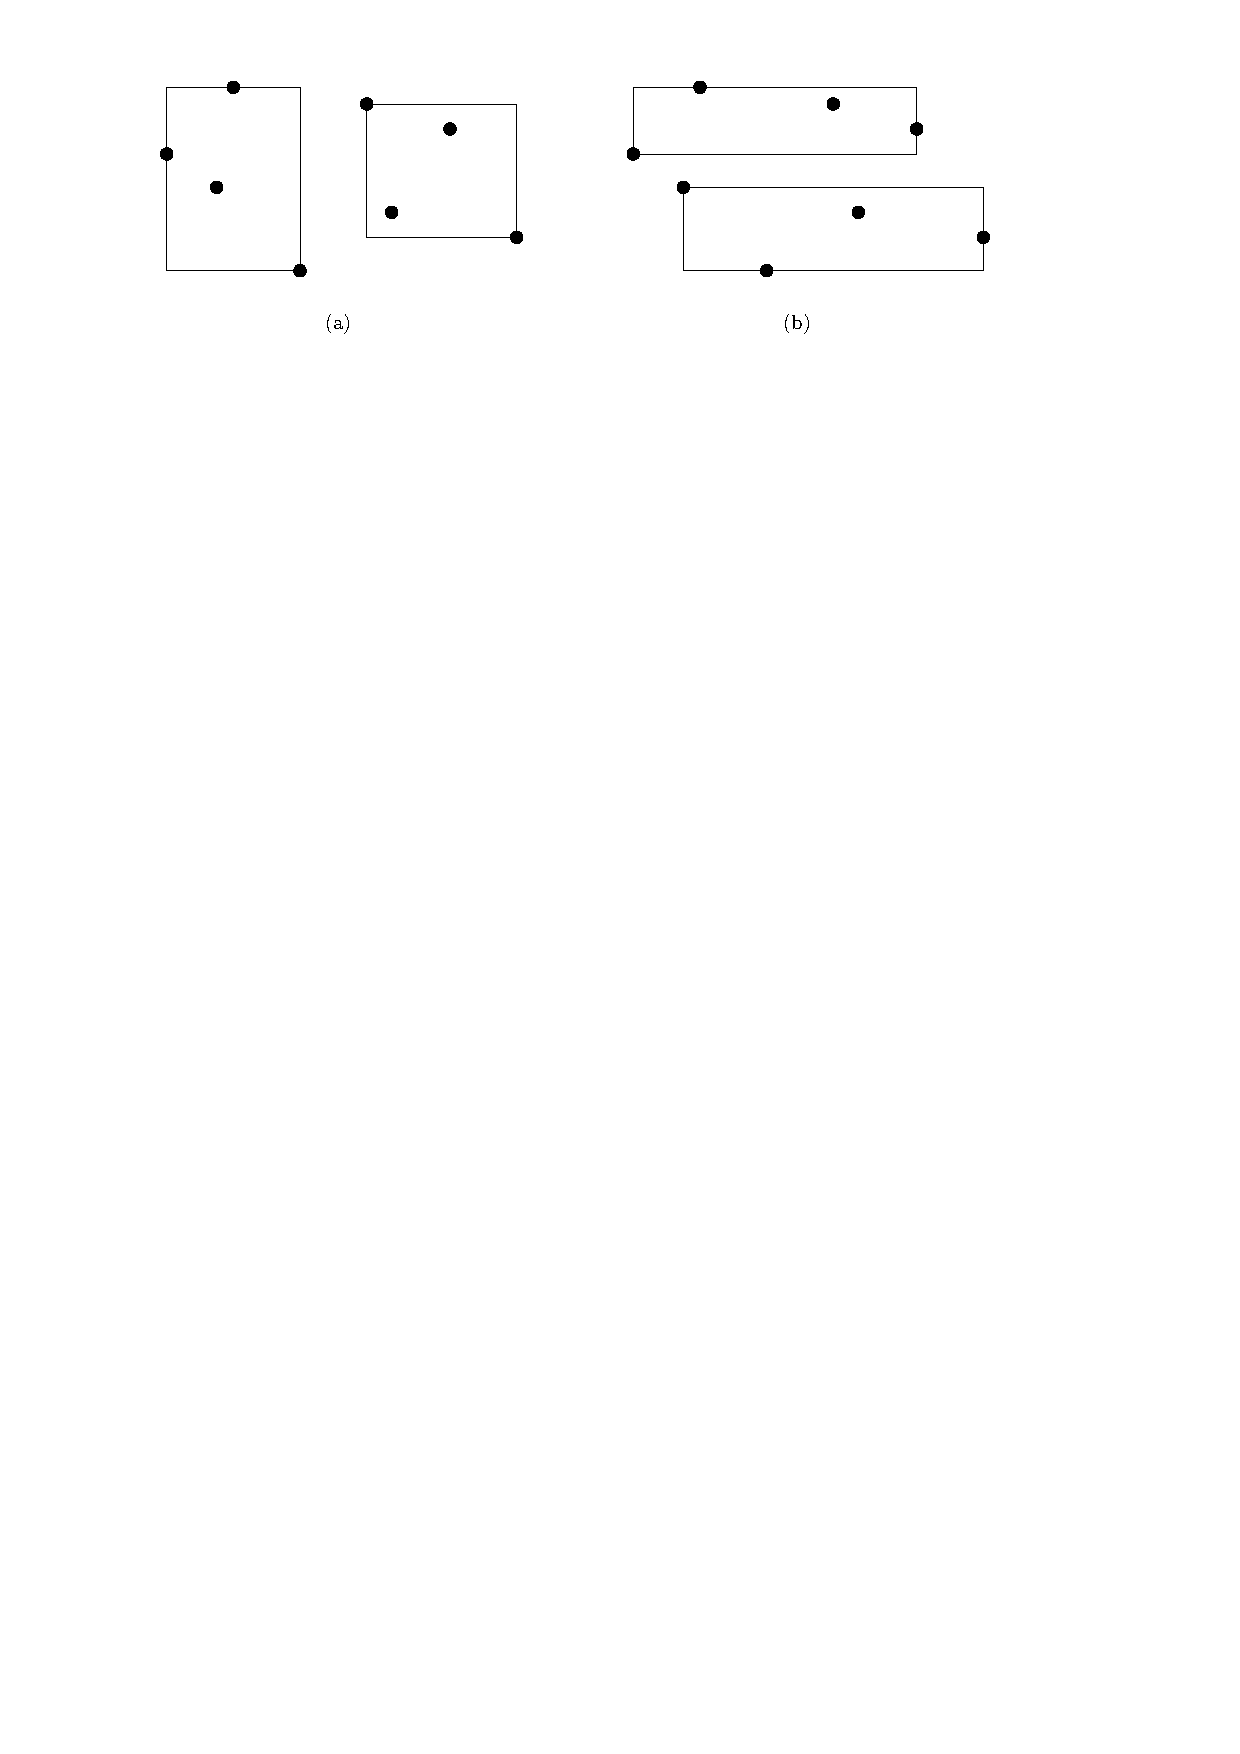
\includegraphics[width=\textwidth]{../figures/r_tree_splitting}
     \caption{(a) Split by cutting the $x$-dimension (b) Split by cutting the $y$-dimension}
     \label{fig:r_tree_splitting}
\end{figure}

\subsection{Deletions}
Let $p$ be the point to be deleted. First the leaf node $u$ which stores $p$ is found using $p$ as search region. Then $p$ is removed from $u$. The deletion is finished if the node has $\lambda B$ points, where $\lambda$ denotes the minimum node utilization. Otherwise, $u$ \textit{underflows}, which is handled by first removing $u$ from its parent, and then re-inserting all points in $u$ using the insert algorithm described above. Now, removing $u$ from from $parent(u)$ may cause $parent(u)$ to underflow too. In general, the underflow of a non-leaf node $u'$ is also handled by re-insertions, with the only difference that the items re-inserted are MBRs, and each MBR is re-inserted to the same level of $u'$.

\section{MySQL}
\label{sec:mysql}
MySQL is a very popular open-source relational database management system. We will not give an in depth description of how relational databases work but we will describe how to very simply adapted MySQL to answer three-sided range queries. A very minimal table was constructed with just two columns. One for the $x$ coordinate and one for the $y$ coordinate. Inserting in the table was done using simple \texttt{INSERT INTO table VALUES \{ values \}} SQL queries. In order to make this work efficiently we buffer inserts in memory and bulk insert whenever the buffer overflows. This gave a significant speedup. Deletion was done similarly simple using \texttt{DELETE FROM table WHERE (x,y) IN \{ values \}} and buffers on top.

Queries of the form $\left[x_1,x_2\right] \times \left[y_1,\infty\right]$ were answered using a \texttt{SELECT * FROM table WHERE $x_1$ <= x AND x <= $x_2$ AND y >= $y_1$}.

\subsection{Analysis}
It is important to keep an open connection to the server at all times or you will end up spending a lot of time reconnecting to the server.

Inserting points in the database involves sending the query to the server, parsing the query, and finally inserting the rows. None of these operations depend on the size of the database as no indices were created on the data. As we buffer inserts together we get an amortized insertion time of $\mathcal{O}(1)$ I/O's.

Deleting points is however very expensive due to the missing index on the data as there is no real way of finding the point in the database without searching through it all. This gives the very expensive $\mathcal{O}(N/B)$ I/O's amortized bound for deleting points.

The same goes for querying the database as we once again have to go through every single point in the database to test if it is in the query range. This also gives an $\mathcal{O}(N/B)$ I/O's bound.

\chapter{Experimental setup}
\label{chp:experimental_setup}
Running experiments on I/O algorithms is extremely time consuming. In order to compare I/O efficient algorithms against internal memory algorithms we need input sizes that force the internal memory algorithms to store and load data to and from the disk (swapping). The input size to the algorithms can be severely minimized if run on machines with a small amount of internal memory.

It is important to mention some considerations when it comes to choice of persistent storage media. In recent years solid state drives have grown increasingly more desirably in terms of price per gigabyte and storage size, but there is still a significant gap in price between SSD's and HDD's. Disregarding this gap in price, solid state drives clearly outperforms the hard disk in every notable aspect. Solid state drives allow random access to blocks and diminish the seek time which is considered to be the culprit of the mechanical disks due to the rotational latency.
The rotational latency makes it very important to store data on the disk in consecutive blocks as scattering data across the disk would be detrimental to the performance as each block would have to be wait for the rotational latency. As long as the mechanical disk is still as widespread as it is, these culprits of the mechanical disk have to be taken in consideration when designing I/O efficient algorithms.

With these considerations in mind we acquired two very old Dell machines with the following specifications:

\begin{figure}[h]
\centering
\begin{tabular}{ll}
CPU & Intel(R) Celeron(R) CPU 3.06GHz \\
CPU L1 cache & 16KiB \\
CPU L2 cache & 256KiB \\
RAM & 512MiB DDR 553MHz \\
Disk & Seagate ST3160828AS \\
Disk capacity & 160GiB \\
Disk number of disks & 2 \\
Disk number of heads & 4 \\
Disk RPM & 7200 \\
Disk rotation time & 8.33ms \\
Disk seek time & 8.5ms \\
Disk buffer size & 8192KiB \\
Disk sector size & 512bytes \\
Operating system & 32 bit Ubuntu 14.04 \\
Kernel version & 4.2.0-27-generic \\
Compiler & gcc 4.8.4 with optimization level 2
\end{tabular}
\caption{Specifications of the two Dell machines used for running experiments}
\end{figure}

We measured the running time using the \texttt{high\_resolution\_clock} in the \texttt{chrono} library. It was measured in seconds as more precision was not needed in order to distinguish the algorithms as will become apparent in the presented results.

In order to obtain a deeper understanding of the results we chose to measure the number of page faults generated by running the algorithms. This was done using \texttt{perf} - a performance analysis tool for Linux. We also measured the number of I/O's required by our program using the \texttt{/proc/} file system. The number of I/O's was obtained through \texttt{/proc/\{pid\}/io} which gives an approximate number of calls to the system calls \texttt{read} and \texttt{write} by the process.

\chapter{Our results}
Many experiments were conducted to evaluate the performance of the structures against each other. We will in this chapter present the results of these experiments and discuss the results.
Some of the experiments will only be run for 24 hours and not up to a specific amount of data. This was a necessary restriction on the experiments as we otherwise would never have finished or had been able to run many of the experiments we had planned. Some of the data structures become extremely slow when not run in internal memory. This will become very apparent in many of the results shown below.

\section{Parameter tuning}
In order to compare the structures' best performance against each other we needed to find the optimal parameters to run the structures on. The parameters of the structures were mainly the size of the buffer and for the tree structures it was also the size of the fanout in the nodes. These parameters are highly machine dependent as larger main memory allows for larger buffer sizes. 

\todo{change data size when larger results are added}

The experiments consist of inserting 5Gb of data. The data is uniformly random generated among the positive integers.

In Subsection~\ref{subsec:tuning_gerth} we present our tuning parameters for the structure presented in Chapter~\ref{chp:epst} by Brodal, and in Subsection~\ref{subsec:tuning_arge} we present our findings for the structure presented in Chapter~\ref{chp:arge_pst} by Arge et al.

\subsection{External memory buffered priority search tree}
\label{subsec:tuning_gerth}

\begin{figure}[htp]
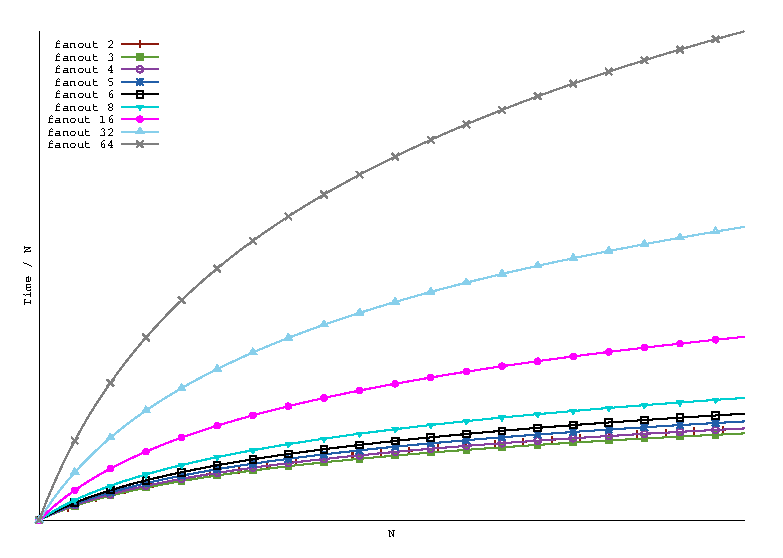
\includegraphics[width=\textwidth]{../plots/gerth_update_epsilon/gerth_epsilon}
\caption{Theoretical update time for different fanouts (epsilon).}
\label{fig:gerth_fanout_theory}

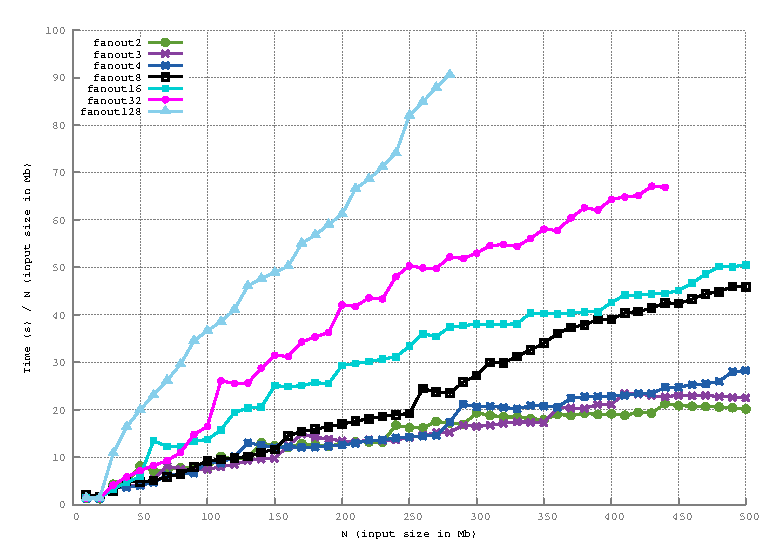
\includegraphics[width=\textwidth]{../src/experiments/gerth_fanout_experiment_results/2016-04-21.15_38_18/time_over_input}
\caption{Running the data structure of Brodal with a fixed buffer size at 8Mb and varying fanouts.}
\label{fig:gerth_fanout_experiment}
\end{figure}

\begin{figure}[htp]
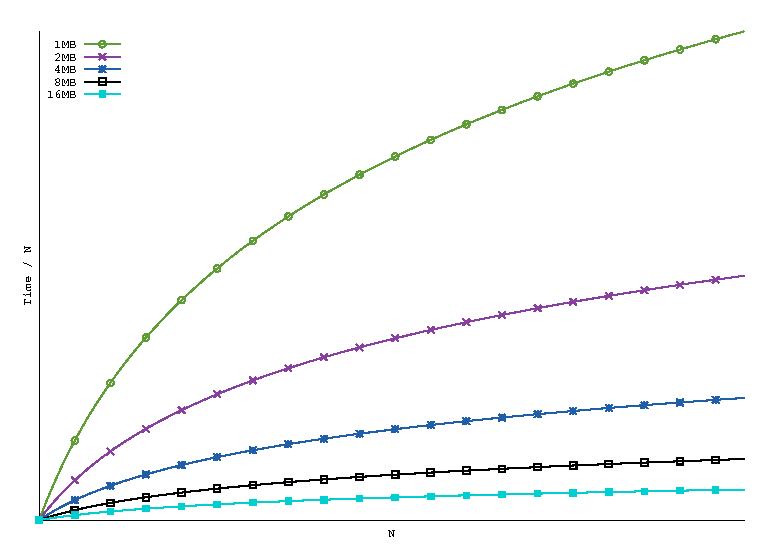
\includegraphics[width=\textwidth]{../plots/gerth_update_buffer_size/gerth_buffer_size}
\caption{Theoretical update time for different buffer sizes.}
\label{fig:gerth_buffer_size_theory}

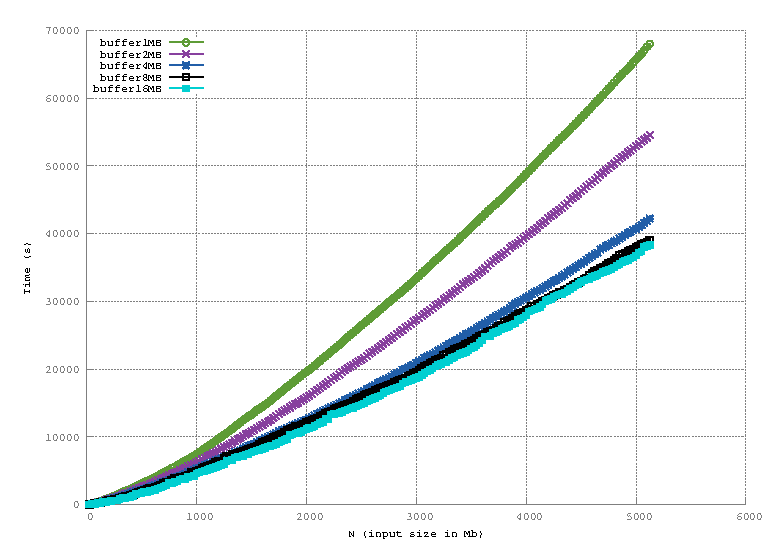
\includegraphics[width=\textwidth]{../src/experiments/gerth_buffer_size_experiment_results/2016-05-03.13_51_54/time}
\caption{Running the data structure of Brodal with a maximum fanout of 2 and varying buffer sizes.}
\label{fig:gerth_buffer_size_experiment}
\end{figure}

Figure~\ref{fig:gerth_fanout_experiment} shows that the running time increases as the fanout increases. This is very much in line with the theoretical bounds as depicted in Figure~\ref{fig:gerth_fanout_theory} and fits very well with the overall intuition that being able to send more points down on each overflow is key to increasing performance. The tree might increase significantly in height but we decrease the frequency of overflow in the root. It is also worth noting that smaller fanouts allow for larger buffer sizes as the child structures does not take up as much space if we do not have that many children.

\todo{Do some math on this to show that the number of overflow decreases}
\todo{Add plots of gerth statistics}
\todo{Explain these results with the code in mind. Smaller fanout sends more points down at a time}
\todo{Add the formulas that are plotted to text}

In Figure~\ref{fig:gerth_buffer_size_experiment} we fixed the fanout to 2 and varied the buffer size. Theoretically the running time should decrease with ever increasing buffer sizes as shown in Figure~\ref{fig:gerth_buffer_size_theory}. We are however limited by the main memory size and we have to be careful not to start swapping out memory to disk as this greatly decreases performance.

\begin{figure}[htp]
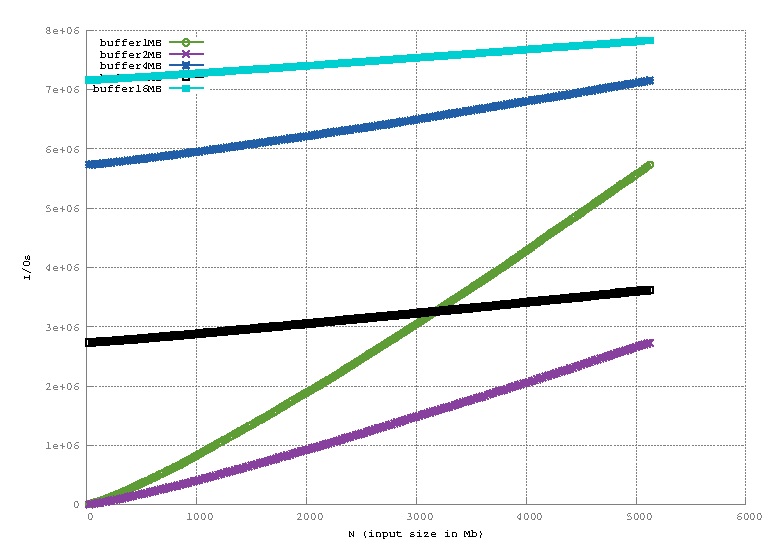
\includegraphics[width=\textwidth]{../src/experiments/gerth_buffer_size_experiment_results/2016-05-03.13_51_54/ios}
\caption{Number of calls to read and writ for different buffer sizes.}
\label{fig:gerth_buffer_size_ios}

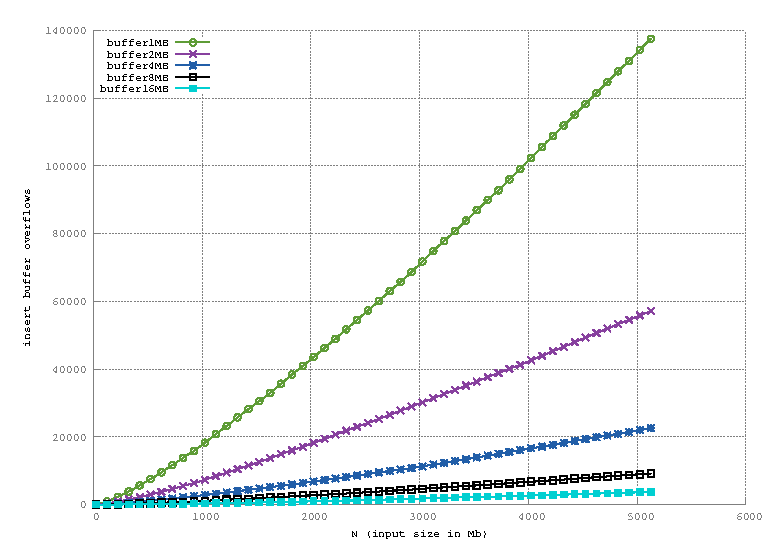
\includegraphics[width=\textwidth]{../src/experiments/gerth_buffer_size_experiment_results/2016-05-03.13_51_54/ibo}
\caption{Number of insert buffer overflows in the structure of Brodal.}
\label{fig:gerth_buffer_size_ibo}
\end{figure}

Figure~\ref{fig:gerth_buffer_size_ios} aligns very well with the actual running time and our expectations. The number of I/O's decreases with increasing buffer sizes.

Figure~\ref{fig:gerth_buffer_size_ibo} show the number of times an insertion buffer overflows. In fact we see a similar decrease in the number of operations in all of the update operations described in Subsection~\ref{subsec:gerth_updates}.

\todo{This is also what we see in Figure~\ref{fig:gerth_buffer_size_experiment} where the running time decreases as the buffer size increases until we reach 8Mb. At this point the we started swapping out structures and the performance decreased. Larger buffer sizes was also tried but were simply too slow to measure.}

\section{Insertion}
\begin{figure}[htp!]
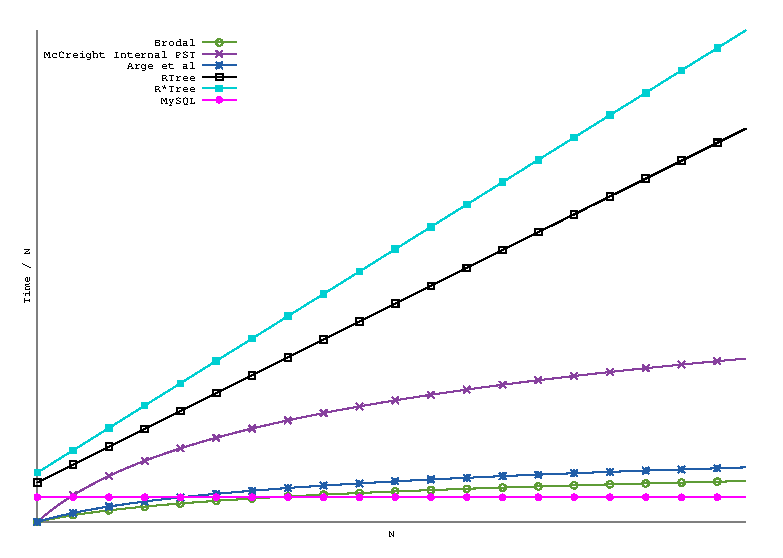
\includegraphics[width=\textwidth]{../plots/insert_complexities/insert_complexity}
\caption{Theoretical insert time for all tested structures.}
\label{fig:theory_insert_complexity}
\end{figure}

Figure ~\ref{fig:theory_insert_complexity} shows the theoretical complexities of inserting an element into the different structures for different $N$. We expect the actual running times to be very similar to these. The experiment will consist of inserting uniformly random data for 24 hours. If the non-I/O efficient data structures fill out the internal memory we expect to see some jumps in the running time at this point.


\section{Deletion}
\begin{figure}[htp!]
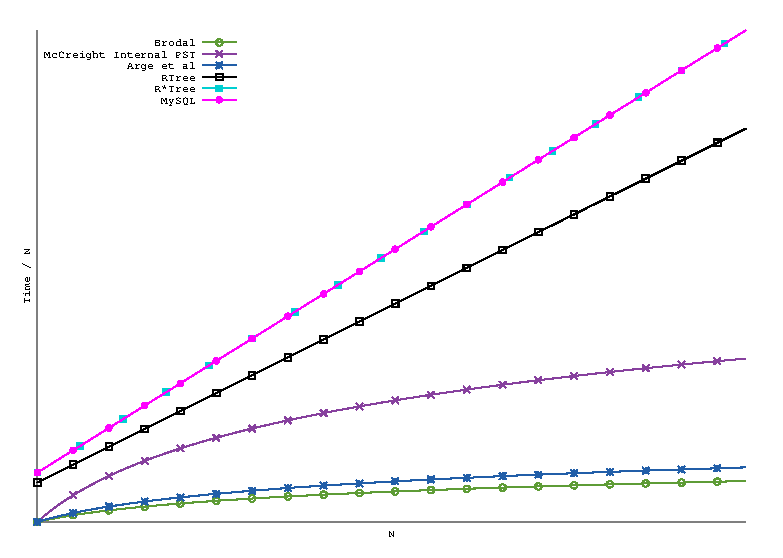
\includegraphics[width=\textwidth]{../plots/delete_complexities/delete_complexity}
\caption{Theoretical delete time for all tested structures.}
\label{fig:theory_delete_complexity}
\end{figure}

\section{Three-sided range queries}
Since the analysis of the theoretical query bounds are done using filtering, we conduct test that focuses both on the \textit{search} and the \textit{report} part of the algorithms. Please refer to section~\ref{sec:filtering} for a description of the method of filtering.

\subsection{Uniform reporting}
The experiment on the \textbf{search} part of the algorithms was conducted by first inserting data \textit{inside} 5 fixed query windows of 5 Mb each. This was followed by inserting uniformly distributed data \textit{outside} the fixed query windows. For insertion of every 10 Mb we report all reports inside the fixed query windows giving a total of 25 Mb reported points. The idea is that we report on both small and large ranges and high and low in the tree. Please refer to figure~\ref{fig:experiment_query_uniform} for an illustration of the distribution of data points. We make sure to stop all clocks when inserting such that our measures only reflect the actual reporting being done.

\begin{figure}[h]
	\centering
	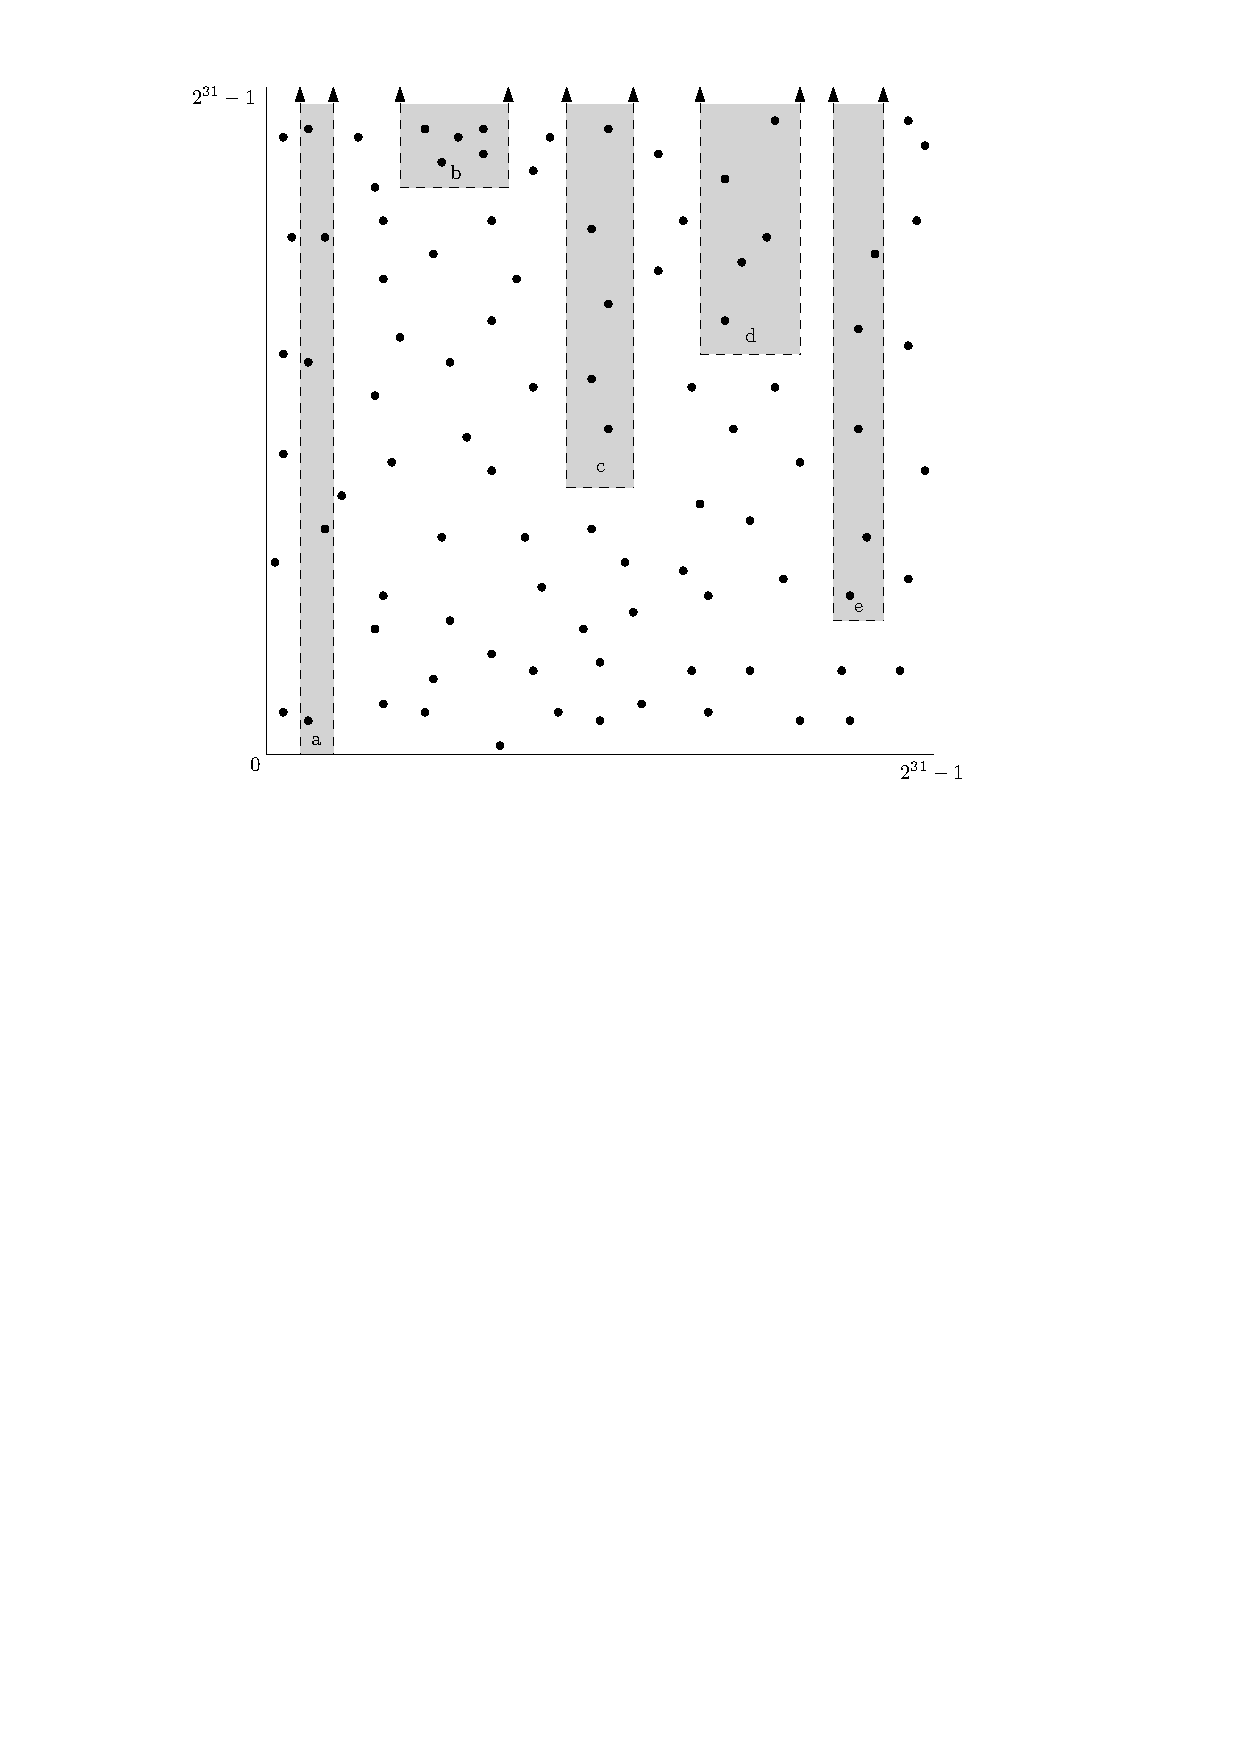
\includegraphics[width=0.8\textwidth]{../figures/query_uniform}
	\caption{Distribution of points for the uniform reporting experiment (search). The gray areas (a) - (e) contains 5 Mb points each. Points are distributed uniformly random. The query window (a) spans 5 \% of the $x$-axis and 100 \% of the $y$-axis (b) spans 17 \% of the $x$-axis and 20 \% of the $y$-axis (c) spans 11 \% of the $x$-axis and 60 \% of the $y$-axis (d) spans 14 \% of the $x$-axis and 40 \% of the $y$-axis (e) spans 8 \% of the $x$-axis and 80 \% of the $y$-axis.}
	\label{fig:experiment_query_uniform}
\end{figure}

The experiment on the \textbf{report} part of the algorithms was conducted by fixing $x_1$, $x_2$ and $y_1, \cdots y_n$ and inserting data points such that there is exactly 
1 Mb data points in the range $[x_1, x_2] \times [y_i, y_{i+1}]$. In the range outside  $[x_1, x_2] \times [- \infty, \infty]$ we distribute data points uniformly at random. Now we report points in ranges $[x_1, x_2] \times [y_1, \infty]$, $[x_1, x_2] \times [y_2, \infty]$ $\cdots$ $[x_1, x_2] \times [y_n, \infty]$. The idea is that the number of reported points $K$ grows with 1 Mb when reporting in the range $[x_1, x_2] \times [y_i, y_{i+1}]$ compared to reporting in the range $[x_1, x_2] \times [y_i, y_{i}]$.

\begin{figure}[h]
	\centering
	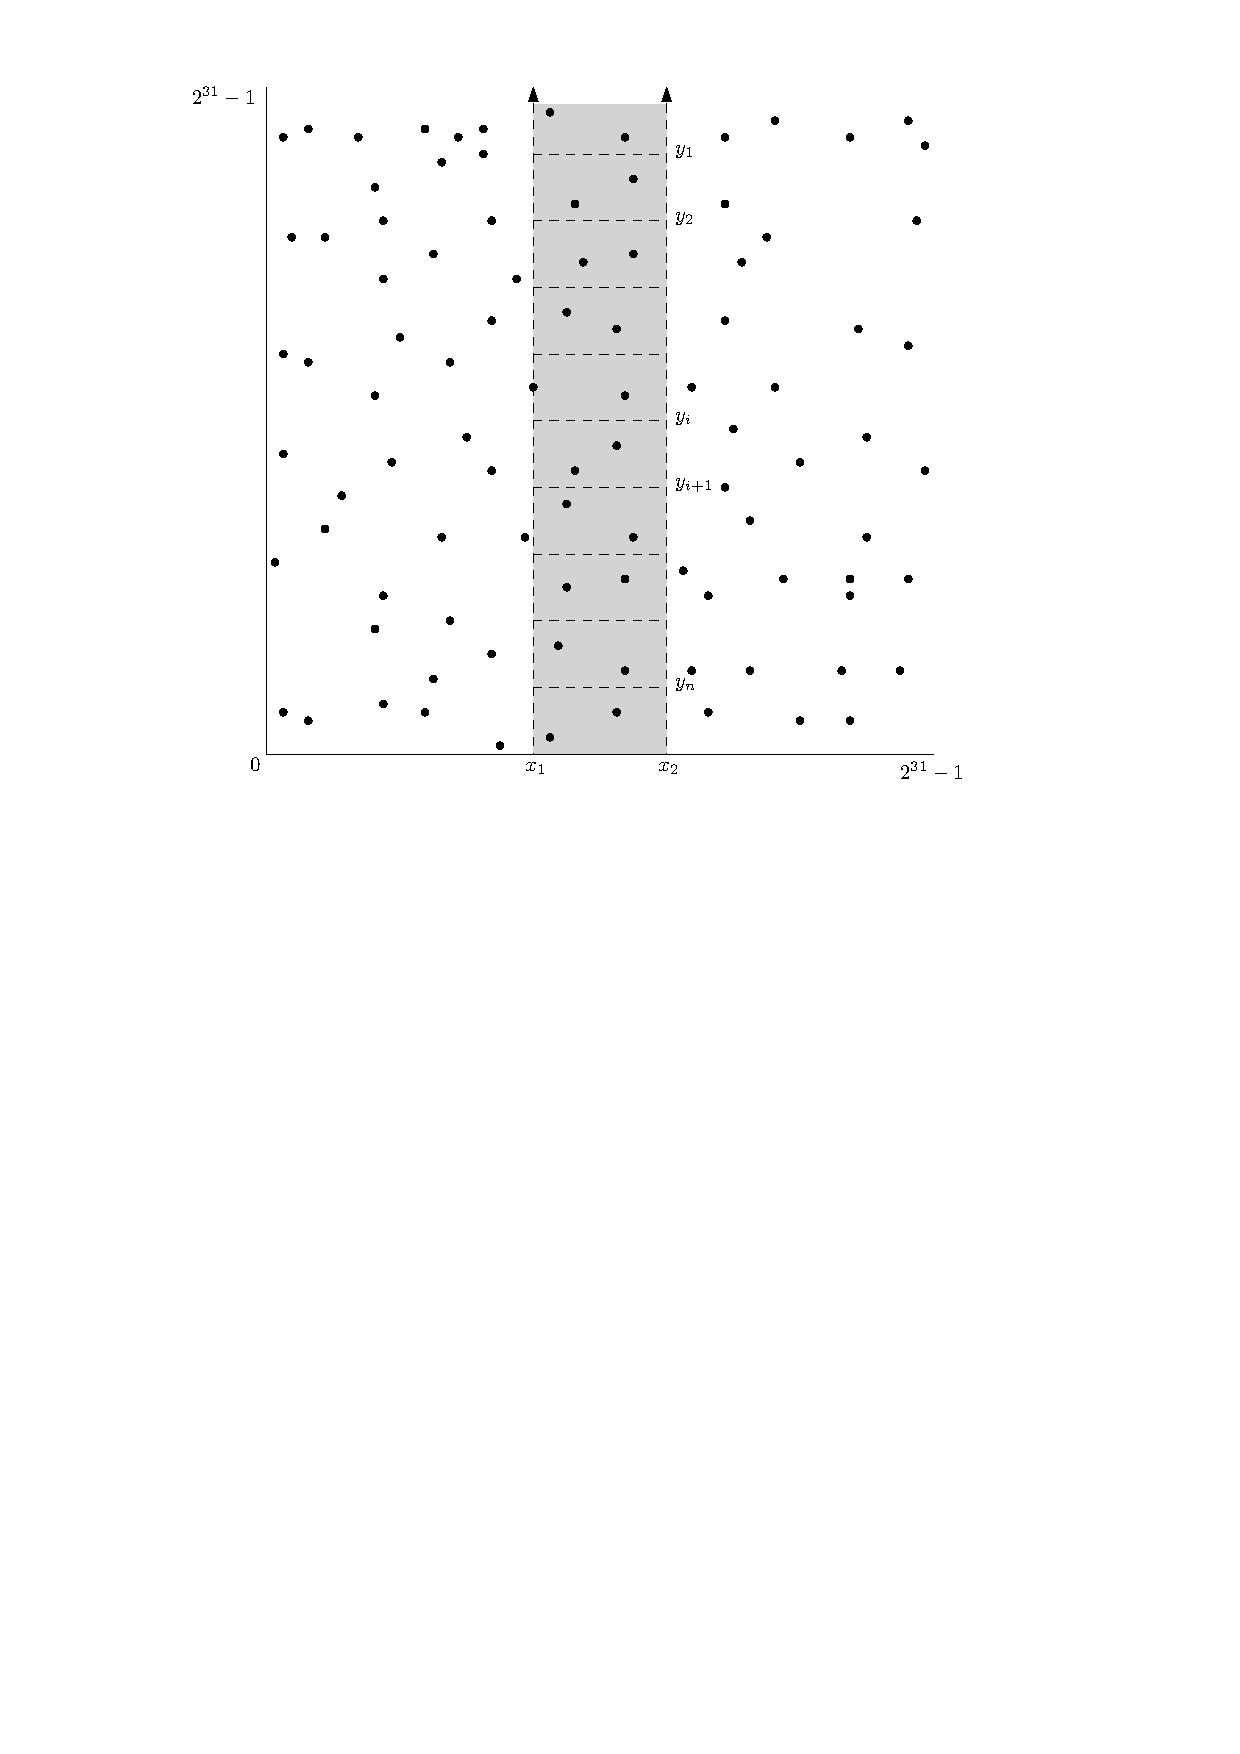
\includegraphics[width=0.8\textwidth]{../figures/query_uniform_fix_x}
	\caption{Distribution of points for the uniform reporting experiment (reporting). The points $x_1, x_2$ and $y_1, \cdots y_n$ are fixed. There is 1 Mb data in all ranges $[x_1, x_2] \times [y_i, y_{i+1}]$}.
	\label{fig:experiment_query_uniform_fix_x}
\end{figure}


\begin{figure}[htp!]
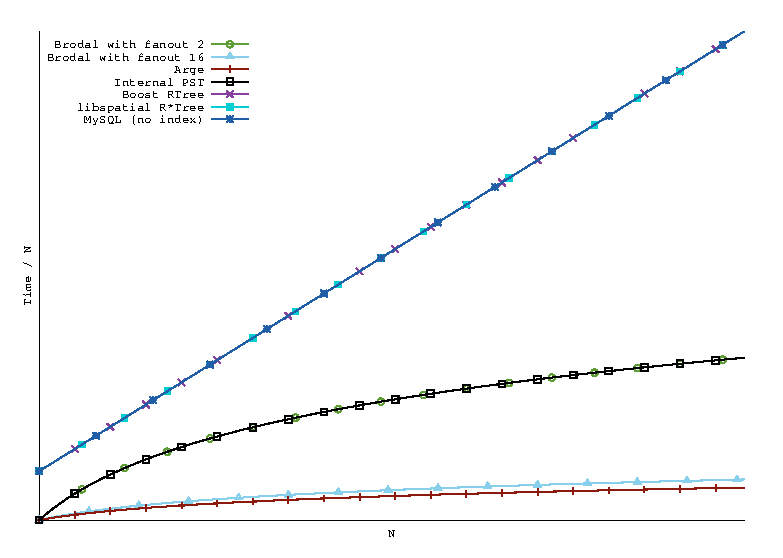
\includegraphics[width=\textwidth]{../plots/query_complexities/query_complexity}
\caption{Theoretical query time for all tested structures.}
\label{fig:theory_query_complexity}
\end{figure}

\subsection{External memory priority search tree}
\label{subsec:tuning_arge}
\todo{add figure and explain results of Arge}

\chapter{Implementation considerations}
%TODO We use a POSIX file-system on a Linux distribution.

\section{Stream}
The implementation we present makes use of the concept of \textit{streams}. A stream gives access to reading and writing from/to disk to/from memory. A stream typically manages an internal buffer which is a mirror a small portion of the disk allowing for fast interaction with that small piece. Although the C++ standard library provides several streams that allow for the internal buffer to be managed we introduce an implementation of our own. We denote this stream \texttt{buffered\_stream}. This design choice was made because of the nature of our experiments in which it is of extreme importance that we are able to argue about the exact number of I/O's being used. By introducing a stream of our own we avoid that any undefined behaviour in the standard library implementations gives rise to a potential I/O overhead. Such an overhead would be reflected directly in the overall running time of our implementation.

The stream we introduce makes use of the \texttt{read} and \texttt{write} system calls and is equipped with a buffer of size $B$ in internal memory that is maintained on all operations.

There are many different ways to construct a stream. In order to substantiate our choice of using buffering on top of the \texttt{read} and \texttt{write} system calls we conducted some experiments with some different types of streams:

\begin{itemize}
	\item Direct invocation of the operating system call \texttt{read} and \texttt{write} that reads/writes one item using no buffering mechanism.
	\item The standard library streams \texttt{fread} and \texttt{fwrite} that uses a built-in buffering mechanism that we do not manage.
	\item Direct invocation of the operating system call \texttt{mmap} and \texttt{munmap} that makes use of the operating systems virtual memory mechanism through demand paging.
\end{itemize}

It is clear that direct invocation of the \texttt{read} and \texttt{write} system calls cannot be better than adding buffering on top, which early experiments without doubt showed. The results were so slow that we had to exclude them.

\begin{figure}
  \centering
  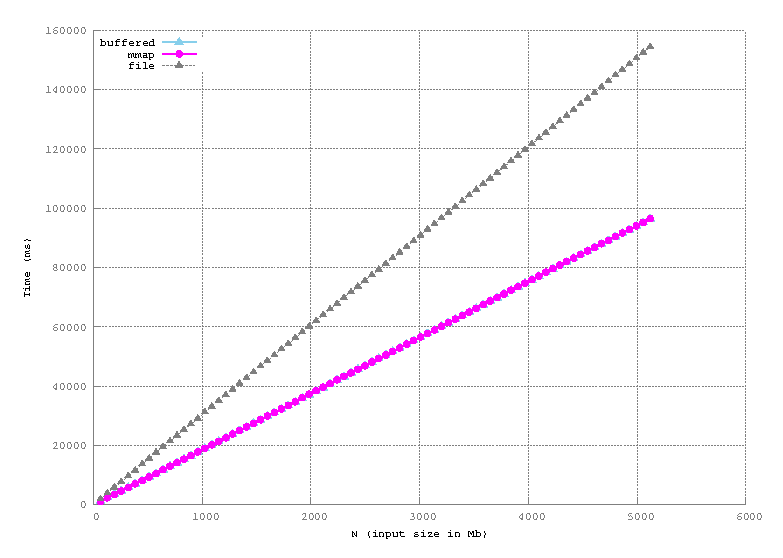
\includegraphics[width=\linewidth]{../src/experiments/stream_input_speed_experiment_results/2016-04-23.16_00_16/timems}
  \caption{Reading 5Gb of data using \texttt{mmap} and \texttt{munmap}, \texttt{fread} and \texttt{fwrite}, and buffered \texttt{read} and \texttt{write}}
  \label{fig:stream_input_speed}
\end{figure}

\begin{figure}
  \centering
  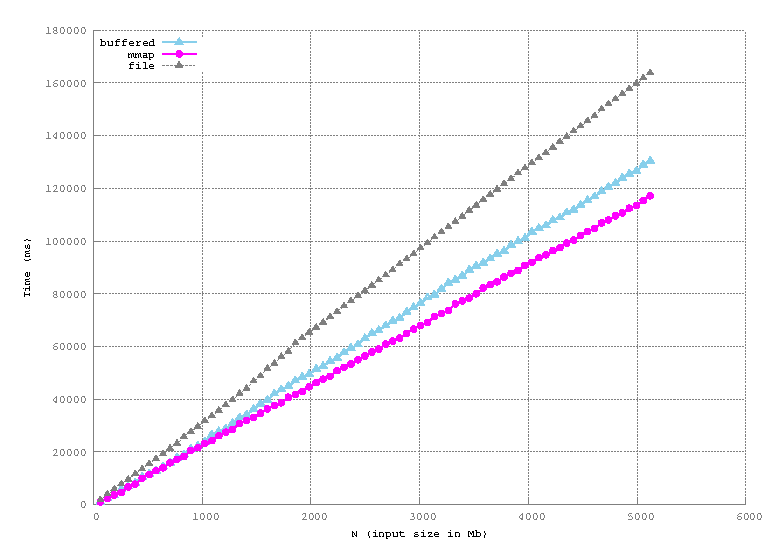
\includegraphics[width=\linewidth]{../src/experiments/stream_output_speed_experiment_results/2016-04-23.16_07_40/timems}
  \caption{Writing 5Gb of data using \texttt{mmap} and \texttt{munmap}, \texttt{fread} and \texttt{fwrite}, and buffered \texttt{read} and \texttt{write}}
  \label{fig:stream_output_speed}
\end{figure}

The results of Figure~\ref{fig:stream_input_speed} and~\ref{fig:stream_output_speed} shows that the \texttt{buffered\_stream} performs similarly to using \texttt{mmap} when reading 5Gb of data.

\todo{talk about results on SSD disks and newer computers}

\todo{comments on the results}

\todo{this is not the case when we have queries in the child structure which relies on seek.}

\todo{Redo experiments and comment on those.}

\section{Child structure}
This section will present the implementation specific design choices made for the child structure presented in section~\ref{sec:child_structure}. \\

\textbf{The initial splitting} of points into blocks of size $B$ is done in a single scan of the x-sorted points. During the scan we make sure to keep track of the minimum and maximum x-value in the range of each block.

\textbf{The catalog data structure} is updated with an entry for each block with information about the minimum and maximum x-value and the indices into a vector $L$ containing all points.

\textbf{Sweeping} of the y-axis is done from bottom to top using a priority queue from the C++ standard library. Initially we put all points in the priority queue keyed on the y-value and with an auxiliary information about the block it initially belonged to. When popping an element we make sure to maintain a counter on the most recent block holding the element. This allows us to collapse adjacent blocks.

\textbf{Maintainance of blocks} is done using a Red-Black search tree $\mathcal{T}$ on block id. When partitioning the $\vert L \vert$ points into $\ell = \lceil\lvert L \lvert / B\rceil$ blocks we initially construct $T$ on data points $1, 2, \dots, \ell$. As each point carries information about the block id it initially belonged to, we are able to find adjacent blocks using a \texttt{successor} and \texttt{predecessor} query on block id in $\mathcal{T}$. Whenever the sweepline reaches a point in a block where the block together with an adjacent block contains exactly $B$ points on or above the sweepline, we either fusion with the block on the left, with the block on the right, or with both the block on left and the block on right. When fusing with the left block we simply delete the block id for the current block in $\mathcal{T}$. When fusing with a right block we delete the successor of the current block id. When fusing with both a left and right block we delete both the current block id and the successor of the current block id. This idea is inspired by the concept of interval trees presented in ?????. %TODO Inds�t reference
Every time a fusion of blocks is caused we create a copy of all points belonging to the new block to the back of $L$. For the newly created block we update the \texttt{catalog structure} with information about the minimum y-value, the block id of the initial left-most and right-most block being covered and indices into $L$.
It is clear we always create at least one less block whenever we fusion. This gives a total of $\mathcal{O}(\ell) = \mathcal{O}(B^{\epsilon})$ blocks.

\textbf{Updates} are delayed by storing them in the $\mathcal{I}$ or $\mathcal{D}$ buffers, respectively. Whenever $\mathcal{I}$ or $\mathcal{D}$ have more than $B$ points, we simply extract the points $L$ in $\mathcal{L}$ in increasing x-order from the blocks $b_1, \dots, b_{\ell}$ in $\mathcal{O}(\ell)$ I/O's and apply the $\mathcal{O}(B)$ updates. In order to rebuild the data structure we perform the construction exactly as described above initially splitting the points into $b_1, \dots, b_{\ell'}$ blocks. The fusion of blocks takes $\mathcal{O}(1)$ I/O per block implying reconstruction takes worst-case $\mathcal{O}(\ell')$ I/O's. Since $\lvert L \lvert = \mathcal{O}(B^{1+\epsilon})$ and the reconstruction of $\mathcal{L}$ whenever a buffer overflows requires $\mathcal{O}(\lvert L \lvert / B) = \mathcal{O}(B^{\epsilon})$ I/O's, the amortized cost of reconstructing $\mathcal{L}$ is $\mathcal{O}(1/B^{1-\epsilon})$ I/O's per buffered update.

\textbf{Queries} are answered by scanning the \texttt{catalog structure} from right to left. During the scan we maintain a bit-vector of size $\ell = \lceil\lvert L \lvert / B\rceil$ that marks the blocks covered by a catalog entry overlapping the x-range of the query interval. We do not consider catalog entries if their starting block id is marked, as this implies the entire block is already spanned by a marked block. This follows directly from the fact we always expand the range of the block introduced by collapsing. 

\begin{lemma}
\label{lma:no_splits}
When visiting blocks from most recent collapsed block to least recent collapsed block, it is always sufficient to test whether the start or end index of a block is marked to check if the entire block has been covered.
\end{lemma}

Proof of Lemma~\ref{lma:no_splits}. Assume for contradiction a block $b_{ij}$ has marked[$i$] = marked[$j$] = 1 and marked[$k$] = 0 for  $i < k < j$. The assumption basically states we have chosen a block $b_{ij}$ with a marked start-index and end-index and with part of the block being unmarked. Then we must have split a block before arriving at the block in question. This contradicts the fact that we always collapse (and thus never splits) blocks. $\square$ \\

If the catalog item considered is non-marked and if the minimum-y value is strictly below the y-value from the query, then we report all points in the query-range from the block. As we scan the \texttt{catalog structure} from right to left we are ensured to mark and report from the blocks being intersected by the query-y. \\

\textbf{The reporting} is done using the point indices stored in the \texttt{catalog structure}. If the point set $L$ has been read into main memory then we report the points directly from $L$, if not, we make sure to \texttt{seek} to the start-index in the file containing $L$ such that we only read in the $\leq B$ consecutive points that are candidates for being reported.
We charge $\mathcal{O}(1)$ I/O's for accessing the \texttt{catalog structure} and $\mathcal{O}(K/B)$ I/O's for reporting points from the query range. This gives a total of  $\mathcal{O}(1+K/B)$ I/O's for querying.

\section{Main data structure}
\label{sec:impl_main_data_structure}
This section will present the implementation specific design choices for the main data structure presented in section~\ref{sec:main_data_structure}. \\

In section~\ref{sec:main_data_structure} we argued how the operations \texttt{Insert}, \texttt{Delete} and \texttt{Report} are supported using subroutines for handling overflowing deletion buffers, overflowing insertion buffers, split leaves with overflowing point buffers, split nodes of degree $\Delta+1$ and fill underflowing point buffers.

The implementation we present uses the same idea of introducing a delegated subroutine which is responsible for maintaining one event only.

% introduce dependency mechanism (partly load/flush node).
We decided to implement a \textbf{dependency mechanism} on each node that allows for the node to be partly flushed and loaded. This allows us to optimize the number of I/O's being made as we can restrict the load and flush to be done only on needed data. The data for each node naturally groups into a separate stream for the insert buffer, delete buffer, point buffer, meta data on children and meta data for the node itself. %TODO We will argue in section ?? exactly why the grouping is done as described here.

% introduce event loop
As described in section~\ref{sec:main_data_structure} we have to enable a mechanism that allows for subroutines to call each other, as one event can cause other events to be risen. If we simply let each subroutine call using a na\"{\i}ve call stack we would have to manage that a subroutine can be both caller and callee and so it is responsible for loading and flushing data with respect to the recursion path we are currently on. This would require a logical complex mechanism that does nothing but manage the control flow of the recursion and handling data load and flushing. In order to overcome this we have introduced an \textbf{event loop mechanism} that uses a stack of events to control flush, load and calling  proper subroutines. Using this mechanism we are able to predict exactly what data is needed. Furthermore it becomes an easy task to flush all required data before taking further steps in the recursion ensuring optimal use of available main memory.

% introduce all events
As explained in section~\ref{sec:main_data_structure} we have to make sure that no node in the subtree of a node has a underflowing point buffers before we are allowed to pull up points in the node itself. In order to fully exploit our event loop mechanism we add an extra event for handling the actual pull up of points from the children such that we can distinguish whether we are returning from an underflowing point buffer event or not. Summarising we need mechanisms to handle the following events:

\begin{inlinelist}
	\item handle overflowing deletion buffers
	\item handle overflowing insertion buffers
	\item split nodes of degree $\Delta+1$
	\item fill underflowing point buffers in node
	\item handle point buffer overflow
	\item fill underflowing point buffers in subtree
\end{inlinelist}

% cache abstraction
As it is not uncommon to see consequent events for the same node we have added a \textbf{caching mechanism} that makes sure not to flush data on any nodes used in the previous event if the same nodes and data is required in the current event. This idea of using a simple caching scheme dramatically reduces the number of I/O's required compared against the na\"{\i}ve solution where we load and flush a node completely between each event. \todo{Consider introducing a "cache-hit matrix" with a count of loads/flushes we save on each event or maybe just introduce an example or two?}

% introduce meta info_file
In order to reduce the number of I/O's required we make sure to store a detailed \textit{view} of the state of each node in a separate \textbf{info file} that is maintained on each subroutine. This makes us able to test whether a node is internal or leaf and if it has any broken invariants we should fix using only a single I/O. \todo{Concider introducing an example where we save I/O's.}

% introduce states
As both event loop and buffer over-/underflow thresholds depends on whether we are currently global rebuilding, linear constructing, reporting or handling updates, we introduce a \textbf{state switch} that is used throughout our implementation to decide which path the recursion should take.

% Introduce cascading matrix
As described in section~\ref{sec:main_data_structure} it is clear that handling an event in a node can cause the state in the parent (if any), the node itself and in the children (if any) to change, so we will get cascading events that needs to be handled. We define the subset of nodes that potentially could change state directly caused by handling an event as the \textit{neighborhood} of the node under an event. It is these cascading events on neighbourhoods that ultimately defines the recursion path. It highly depends on the current state of a node what event(s) we need to check in the neighbourhood. Please refer to table~\ref{table:dependency_matrix} for the dependency graph of cascading events depicted as an adjacency matrix. In the matrix we define an internal node with an empty subtree as a \textit{virtual leaf}. Note that this graph is only valid when we are handling insertions an deletions. When handling linear construction, global rebuild and reporting we have to handle a different subset of cascading events.

%TODO Check correctness of this table when not tired!
\begin{table}[]
\centering
\caption{The table depicts which events causes other events to be made in a given node while handling inserts and deletions}
\label{table:dependency_matrix}
\begin{tabular}{lcccc}
\hline
event & root & leaf & virtual leaf & node \\ \hline
(i) & {\color[HTML]{333333} (i), (ii), (vi)} & - & - & (i), (ii), (vi) \\
(ii)  & (ii), (v) & (v), (vi) & (v), (vi) & (ii), (v) \\
(iii)  & \multicolumn{1}{l}{(i), (ii), (iii), (v)} & \multicolumn{1}{l}{(i), (ii), (iii), (v)} & \multicolumn{1}{l}{(i), (ii), (iii), (v)} & \multicolumn{1}{l}{(i), (ii), (iii), (v)} \\
(iv) & (i), (ii) & (i), (ii) & (i), (ii) & (i), (ii) \\
(v)  & (ii) & (ii) & (v) & - \\
(vi)  & (vi) & - & (i), (ii), (vi) & (i), (ii), (vi)
\end{tabular}
\end{table}

\textbf{Updates} are done as described in~\cite{DBLP:journals/corr/Brodal15}[section 4] except for minor divergences. As previously mentioned we denote the state of a node having an empty subtree as the node being a virtual leaf. We distinguish a leaf and a virtual leaf such that we can reuse the empty subtree of a virtual leaf when handling a point buffer overflow. In the case of a point buffer overflow of a virtual leaf we simply pass down $\lceil \nicefrac{B}{B^{\epsilon}} \rceil$ points to an empty child instead of splitting the leaf. In retrospect we could have chosen to delete a node from the data structure when it becomes a virtual leaf which would let the splitting of leafs rebalance the tree. It is clear that a virtual leaf becomes an internal node after handling a point buffer overflow. In order to avoid the node to be point buffer underflowed we define a virtual to become overflown when it has more than $B$ elements. We believe the design choice makes no important impact on the overall performance of the data structure. \todo{Ask Gerth about this}. When inserting and deleting points we ensure to pull up as many points as possible whenever a node point buffer underflows. This means that we pull-up points until one of the following criteria is met: (i) the point buffer of the node has exactly $B$ points (ii) we have emptied a child completely. The second criteria ensures the heap order between point buffers. Please note that even though we have modified the threshold we always pull-up at least $\lceil \nicefrac{B}{B^{\epsilon}} \rceil$ because of the pigeon-hole principle and the fact we underflow a buffer when having less than $\nicefrac{B}{2}$ points. The idea behind this to distribute as many points as close to the root as possible using the same amount of I/O's. \todo{Ask Gerth about this}. As a corner case we handle the initial splitting of the root when having exactly $B+1$ points even though it is technically a leaf and should have been split when the buffer had $\nicefrac{B}{2}$ points. If we had treated the root as a leaf then we would underflow the root immediately after a split causing a looping point buffer underflow event followed by a point buffer overflow event.

\textbf{Reporting} is done using the same ideas as presented in ~\cite{DBLP:journals/corr/Brodal15}[section 6]. In detail this means we report using a breadth-first traversal within the search path of the $x$-axis. We push down points from buffers to children while reporting instead of using two separate sweeps as suggested in ~\cite{DBLP:journals/corr/Brodal15}[section 6]. Whenever we identify a child having a lower minimum $y$-point than the query, we avoid recursing on the child. After having reported points we have a main data structure that is most likely very unbalanced because of the flushing of buffers along the search path. We fix this in a bottom-up manner visiting all nodes on the search path. For a given node we fix events in the following order (i) delete buffer overflow , (ii) insert buffer overflow, (iii) node degree overflow, (iv) point buffer overflow. We disallow the recursion to travel above the current node in question. This means we always maintain the invariant of having a consistent tree below the current node handled. The recursion path it controlled having the \textbf{state switch} set to a fix\_up state.

%%%%%%% General conciderations about the tree.
The \textbf{general representation} of buffers makes use of binary Red-Black search trees (\texttt{set<point>} from the C++ standard library) on totally ordered points. This design choice allows us to retrieve the minimum and maximum element in each buffer in constant time using \texttt{iterator} pointers. Furthermore we are able to traverse each buffer in sorted order in linear time which is needed when computing a subset of points to handle on a buffer overflow and underflow. We are aware that using a search tree comes with the price of space blow-up, as each node needs a pointer for children and parent, giving a total of $32 \cdot N$ bytes extra compared to a \texttt{std::vector<point>} representation. We maintain the point buffer as two separate search trees totally ordered on the $x$-value and $y$-value respectively. This is needed as we frequently need access to the minimum $y$-value when deciding whether we should insert a point into the point buffer or insert buffer. The \textbf{catalog structure} containing information about the children of each node is also represented as a Red-Black search tree on interval-start of the children. In detail each catalog item stores information about the minimum point, minimum $y$-point, maximum $y$-point and node id for each child. In the \textbf{info file} of each node we maintain a bit on whether the node is a leaf, a virtual leaf or an internal node, whether the node currently has an overflowing or underflowing point buffer, overflowing point buffer, insert buffer, delete buffer and whether the node is currently node degree overflowed. This allow the event loop to identify whether we should fix any broken invariants caused by events in the neighbourhood, using only 1 I/O.

As an overall strategy we make sure to pass arguments by reference in order to avoid copying objects to the call stack.

\todo{Explain the overall idea in each event - postponed until we are done with the final implementation}.

\section{External priority search tree of Arge et al.}
Drawing from the experiences gained while implementing the main data structure of Section~\ref{sec:impl_main_data_structure} we decided to once again make use of the event loop to handle our recursion allowing for full control of load and flush. This choice also allowed for simple adaptation of the caching mechanism previously described.

The elements of the base B-tree is a simple type containing a point, a reference to a child, and a bool telling us whether the point has been deleted. The elements are stored in nodes which is just a collection of the simple point types, a reference to a query data structure, and some booleans used in loading and flushing mechanisms. The collection used for the simple point types is a Red-Black tree (\texttt{std::set}). This collection allows us to find the child responsible for a point in logarithmic time using binary search and naturally keeps the points in sorted order w.r.t the $x$-values.

The article uses a different query data structure for leaves in the B-tree. The query data structure used the article is a simple linked list sorted on $y$-values. The linked list however matches the cost of the query data structure used in internal nodes, namely $\mathcal{O}(1 + K/B)$, and we decided the code would be simpler if we used the query data structure in the leaves as well.

Updates and reporting are done as described in Section~\ref{sec:arge_updates} and~\ref{sec:arge_query} with no remarkably deviations.

\clearpage
\addcontentsline{toc}{chapter}{Bibliography}
\bibliography{references}

\end{document}

